% mn2esample.tex
%
% v2.1 released 22nd May 2002 (G. Hutton)
%
% The mnsample.tex file has been amended to highlight
% the proper use of LaTeX2e code with the class file
% and using natbib cross-referencing. These changes
% do not reflect the original paper by A. V. Raveendran.
%
% Previous versions of this sample document were
% compatible with the LaTeX 2.09 style file mn.sty
% v1.2 released 5th September 1994 (M. Reed)
% v1.1 released 18th July 1994
% v1.0 released 28th January 1994

\documentclass[useAMS,usenatbib]{mn2e}
% If your system does not have the AMS fonts version 2.0 installed, then
% remove the useAMS option.
%
% useAMS allows you to obtain upright Greek characters.
% e.g. \umu, \upi etc.  See the section on "Upright Greek characters" in
% this guide for further information.
%
% If you are using AMS 2.0 fonts, bold math letters/symbols are available
% at a larger range of sizes for NFSS release 1 and 2 (using \boldmath or
% preferably \bmath).
%
% The usenatbib command allows the use of Patrick Daly's natbib.sty for
% cross-referencing.
%
% If you wish to typeset the paper in Times font (if you do not have the
% PostScript Type 1 Computer Modern fonts you will need to do this to get
% smoother fonts in a PDF file) then uncomment the next line
% \usepackage{Times}

%%%%% AUTHORS - PLACE YOUR OWN MACROS HERE %%%%%
\newcommand{\conj}[1]{\overline{#1}}
\newcounter{NameOfTheNewCounter}
\setcounter{NameOfTheNewCounter}{1}
\newtheorem{theorem}{Theorem}[NameOfTheNewCounter]
\newtheorem{lemma}[theorem]{Lemma}
\newtheorem{proposition}[theorem]{Proposition}
\newtheorem{corollary}[theorem]{Corollary}
\newtheorem{definition}[theorem]{Definition}
\usepackage{graphicx}
\usepackage[sc]{mathpazo}
\usepackage{amsmath}
\usepackage{graphicx}
\usepackage{caption}
\usepackage[T1]{fontenc}
\usepackage[utf8]{inputenc}
\def\lp{\frac 1 {l_{0}}}
\def\kp{\frac 1 {m_{0}}}
\newcommand{\Gcal}{\bmath{\mathcal{G}}}
\newcommand{\Rcal}{\bmath{\mathcal{R}}}
\newcommand{\Mcal}{\bmath{\mathcal{M}}}
\newcommand{\Fcal}{\bmath{\mathcal{F}}}
\newcommand{\GG}{\bmath{G}}

\newcommand{\aaps}{A\&AS}
\newcommand{\aap}{A\&A}
\newcommand{\mnras}{MNRAS}
\newcommand{\nat}{Nature}
\newcommand{\physrep}{Phys. Rep.}

%%%%%%%%%%%%%%%%%%%%%%%%%%%%%%%%%%%%%%%%%%%%%%%%

\title[Correlator Windowing Functions For Cheaper Surveys]{Signals Correlation Algorithms For Cheaper Surveys: Using Windowing Functions. 
}
\author[M. T. Atemkeng , O. M. Smirnov, C. Tasse, G. Foster and J. Jonas]{M. T. Atemkeng$^{1}$, O. M. Smirnov$^{12}$\thanks{E-mail: 
o.smirnov@ru.ac.za (OMS); m.atemkeng@gmail.com (MTA); cyril.tasse@obspm.fr (CT); griffin.foster@gmail.com (GF); j.jonas@ru.ac.za (JJ)}, 
 C. Tasse$^{123}$, G. Foster$^{12}$, J. Jonas$^{12}$ \\
$^1$Department of Physics and Electronics, Rhodes University, PO Box 94, Grahamstown, 6140, South Africa\\
$^2$SKA South Africa, 3rd Floor, The Park, Park Road, Pinelands, 7405, South Africa\\
$^3$GEPI, Observatoire de Paris, CNRS, Universite Paris Diderot, 5 place Jules Janssen, 92190 Meudon, France}
\begin{document}

\date{in original form 2014 Mai 11}

\pagerange{\pageref{firstpage}--\pageref{lastpage}} \pubyear{2013}

\maketitle

\label{firstpage}

\begin{abstract}
This paper investigates the use of baseline dependent windowing functions in interferometry data to minimize the loss of 
signal amplitude (smearing) when the correlated data is averaged over wide bandwidth and long time. In radio interferometry smearing is 
reduced when a cross-correlator averages the correlated data over narrower bandwidth and shorter integration times. Unfortunately, this 
leads to a huge amount of data to manage and it is becoming a bottleneck for further data processing such as calibration and 
imaging.  With future generation surveys, it is important to investigate the reduction of the output data rate. Therefore, the focus of 
this paper is on the use of baselines dependent windowing functions to keep smearing down at an acceptable extent and at the same time 
significantly suppress signals 
from out field of view sources, while the nominal sensitivity is conserved. 
\end{abstract}
\begin{keywords}
Instrumentation: interferometers, Methods: data analysis, Methods: numerical, Techniques: interferometric
\end{keywords}

\section[]{Introduction}
The recent radio astronomy techniques is to build a single, gigantic instrument called \textit{interferometer}, from the combination of 
several small parabolic antennas separated over kilometres (\cite{2}). The signal from each antenna is combined at the level of a 
cross-correlator to form the interferometer  data output. The cross-correlator carries out  data reduction and filters out an amount of 
noise by averaging the signal of each baseline over discrete time and/or frequency bins.
It is well known in interferometry that averaging 
can lead to the loss of signal amplitude when the cross correlator integrate over a longer period of time and a wider bandwidth. This 
effect is known as time-average smearing and bandwidth smearing (Thompson et \textit{al.} \cite{2}). The above effects cause the distortion 
of sources within the 
field of interest by decreasing their intensity.\\
To keep smearing down at acceptable levels, a correlator must cross-correlate the signal over a shorter period of time and a narrower 
bandwidth, hence producing a large amount of data for subsequence stage such as 
imaging \citep{Marti2008,Linfield1986}, calibration (\cite{2}), etc. This huge amount of data is becoming an increasingly serious 
problem 
and becoming 
more challenging as the computational demands of the next generation radio telescopes will rise significantly (see the SKA phase 1 
specification \cite{2}). 
Similarly, the next generation of radio telescopes will require an unprecedented level of SNR while mapping large regions of the sky. Thus, 
a substantial 
increase in \textit{SNR} can only be achieve by observing for longer time at wider bandwidth without loss of signal: this is not 
realisable with averaging.
Therefore, it becomes urgent to develop new decorrelation algorithm techniques that will allow the required SNR of the future radio 
telescopes.\\
In this paper, we investigate the efficiency of correlator windowing functions for the reduction of 
interferometric data and the recovery of interferometers arrays desire FoV, with the ultimate goal of reaching higher SNR. The main idea is 
to achieve a high SNR by conserving the astrophysical signal and by limiting the noise. Thermal noise can be driven arbitrary low by 
increasing the observing time\footnote{...}, but in radio astronomy confusion noise is a major problem and can even cause calibration to 
fail. Therefore, we seek to use a windowing function that will conserve the useful signal while also limiting sidelobes confusion from out 
of FoV sources.
\begin{equation}
 SNR=\frac{S_{use}}{N_{ter}+N_{con}}
\end{equation}
\begin{itemize}
  \item "\textit{Useful signal}", $S_{use}$ the signal from source in the field of interest. These sources should be accurately recovered
over the instrument entire FoV : correlator windowing functions maximized this signal by allowing the interferometer array to map a large 
region of the sky.
  \item "\textit{Sidelobe confusion}", $N_{con}$ signal from out field of view sources received from their  sidelobes. These sources are  
not of interest and should be removed : correlator windowing functions acts as a remover of these signals when the array is mapping a large 
region of the sky.
  \item "\textit{Thermal noise}", $N_{ter}$ the thermal noise from the instrument, ionosphere, etc. Averaging presents theoretically  a 
maximum sensitivity, but the use of extended correlator windowing functions can reduce or eliminate the loss of the nominal sensitivity.
\end{itemize}
The proposed techniques are applied to MeerKAT (Karoo Array Telescope) \cite{1} and the Very Large 
Array (VLA)\cite{1} and  could also be used for future radio telescopes such as the SKA.
\section[]{ Overviews and definitions}
\subsection{Visibility and relation with the sky }
\label{sec:visSky}
An interferometer array measures a quantity $V=V(u,v,w)$ known classically as the visibility function.
The variables $u,v$ and $w$ are in unit of wavelength and they are the coordinates of the vector of which the norm is the distance between 
two antennas, known in interferometry as a baseline. A source in the sky will see $u$ and $v$ oriented towards the direction East-West and 
South-North respectively and $w$ is directed towards the phase centre of the source plane or image plane. The projection of $u$ and $v$ in 
the image plane are $l$ and $m$ respectively. They are the observed source coordinates, measured in radian. The ideal measurement of 
interferometric wide-field imaging also known as the van Cittert-Zernike theorem \citep{thompson1999fundamentals} is given by
\begin{equation}
 V_{pq,(u,v,w)}=\int \int \frac{I(l,m)}{\sqrt{1-l^2 - m^2}}e^{-2\pi i \phi (u,v,w)}dldm, \label{eq1:visSky}
\end{equation} 
where $I(l,m)$ is the sky brightness and $\phi(u,v,w)=ul+vm+w(\sqrt{1-l^2 - m^2}-1)$ is a term from the cross-correlator that models the 
direction in the sky and the separation of the two antennas. The term $\sqrt{1-l^2 - m^2}$ is the result of the projection of the celestial 
sphere on the image plane.
% 
% In the radio astronomy community, it is well known that the Radio Interferometry Measurement Equation (RIME) description well the 
% visibility equation of a pair of antennas $(p,q)$. After the generic formulation of the RIME by Hamaka et \textit{al}. (), a full sky 
% of the RIME is described mathematically by O.M. Smirnov (2010) and  it is given by
% \begin{equation}
%  V_{pq}=\textbf{G}_{p}\Bigg(\int \int B_{pq}e^{-2\pi i \big(\phi (u,v,w)-w.(\sqrt{1-l^2 - m^2}-1)\big)}dldm\Bigg)\textbf{G}_{pq}^{H}, 
% \label{eq1:visSky},
% \end{equation} 
% $B_{pq}$
\subsection{Averaging and convolution}
\label{sec:AvgCon}
The Earth rotation causes the phase, $\phi (u,v,w)$ to variate in time. The baseline 
coordinates are defined in units of wavelength, and making $\phi (u,v,w)$ to variate in frequency. 
To take this effect into account, Eq. \ref{eq1:visSky} is  rewritten as an integration over time and frequency interval. If we 
consider that $[t_s,t_e]$ is the time integration interval and $[\nu_s,\nu_e]$ the frequency integration 
interval, then Eq.\ref{eq1:visSky} can be re-written as:
% variates in 
% time when the Earth rotation is  if $\textbf{V}_{pq}^{true}(t,\nu)$ is the non integrated visibilities observed during 
% the time interval $\Delta t$ at multi frequency  within the bandwidth $\Delta \nu$, then the cross correlate visibility, 
% $\mathcal{V}_{pq,(t,\nu)}^{corr}$ of the  baseline $(p,q)$ is given as:
\begin{equation}
V_{pq,(t_c,\nu_c)}^{corr}=\frac{1}{\Delta t \Delta \nu} \int_{t_s}^{t_e}\int_{\nu_s}^{\nu_e}V_{pq,(t,\nu)}d\nu dt.
\label{eq2:conti}
\end{equation}
Here, $V_{pq,(t,\nu)}$ is a continuous function, in reality we know only the sampled visibility. Nevertheless, when measuring 
the sampled visibility, the antennas reception pattern or "primary beam", $A_{t,\nu}$ which describes the sensitivity of the interferometer
elements $p$ and $q$, with radius from the centre of the dish beam is taken into account. With this assumption, the  sampled visibility  
measured at discrete spaces is:
\begin{eqnarray}
  V_{pq,(t,\nu)}^{samp}=S_{pq,(t,\nu)}\bigg(V_{pq,(t,\nu)}\circ A_{t,\nu}\bigg),
\end{eqnarray}
where $\circ$ denote the convolution operator and $S_{pq,(t,\nu)}$ is a sampling 
function that indicates where the $(u, v)$ data for the baseline $(p,q)$ are measured  during the integration. It is 
unity where measurement have been made, and zero otherwise.
Therefore, 
Eq.\ref{eq2:conti} holds for many sources, when the signal at the centre frequency and at the centre time is restricted to a narrow 
frequency interval and to a short time interval, this is the current efficient observing mode. However, the mathematics behind is as 
follows: 
\begin{eqnarray}
V_{pq,(t_c,\nu_c)}^{corr}&=&\frac{1}{n_t n_{\nu}}  \sum_{i=1}^{n_t}\sum_{j=1}^{n_{\nu}}V_{pq,(t,\nu)}^{samp}.\label{eq2:sample}
%&=&\frac{1}{n_t n_{\nu}}  \sum_{i=1}^{n_t}\sum_{j=1}^{n_{\nu}}\mathcal{\textbf{V}}_{pq,(t,\nu)}^{meas} 
\end{eqnarray}
Here, $n_t$ and $n_{\nu}$ are the number of discrete times within the time interval  and the number of discrete frequencies 
within the frequency interval  respectively. For convenience, lets introduce a normalized \textit{Boxcar} windowing 
function, $\Pi_{pq,(t_c - t,\nu_c -\nu)}$  that will attribute an equal weight (in this case $1/n_t n_{\nu}$) to all sampling visibilities 
points. We can therefore re-write Eq. \ref{eq2:sample} as:
\begin{eqnarray}
V_{pq,(t_c,\nu_c)}^{corr}&=&\sum_{i=1}^{n_t}\sum_{j=1}^{n_{\nu}}\Pi_{pq,(t_c - t_i,\nu_c -\nu_j)}V_{pq,(t_i,\nu_j)}^{samp}. 
\label{eq:avscon}
\end{eqnarray}
It is worth noting that Eq.\ref{eq:avscon} is a naturally weighted visibility and is a two dimensional convolution between the 
\textit{Boxcar} windowing function and the sampled visibility. Thus, averaging is equivalent to convolving the 
sampled 
visibility with a \textit{Boxcar} windowing function. Mathematically, this is described as follows:
\begin{equation}
 V_{pq,(t_c,\nu_c)}^{corr}=c_{pq,(t,\nu)}\cdot\Bigg(\Big(\Pi_{pq}\circ V_{pq}^{samp}\Big)_{(t,\nu)}\Bigg). \label{f4}
\end{equation}
Here, $c_{pq,(t,\nu)}$ is a function that samples the result of $\Big(\Pi_{pq}\circ V_{pq}^{samp}\Big)_{(t,\nu)}$ at 
the centre time interval and centre frequency interval. 
\\%Its is defined as:$c_{pq,(t_i,\nu_j)}=0$ for \\
%$(t_i,\nu_j)\neq(t_c,\nu_c)$ and $c_{pq,(t_i,\nu_j)}=1$ for $(t_i,\nu_j)=(t_c,\nu_c)$.
Nevertheless, note that this is not an efficient mode of attributing the weight of baselines visibilities. This mean that, the baselines 
of the array are all suppose equally in term of the statistical analyse of the signals from the astronomical source. Unfortunately, this 
is not the case, since we lost informations on some baselines than order due to the incomplete sampling of the Fourier component that 
differ from one baseline to another.
\subsection{Effect of time and bandwidth averaging}
During imaging \citep{briggs1999imaging}, Eq.\ref{f4} is inverse Fourier transform, and the convolution theorem is applied, the 
$sinc$ function therefore multiply the sky (see appendix \ref{label:similarimaging} for a short discussion and illustration). The 
sky map is tapered by the $sinc$ function in the $l$ and $m$ directions, the response is maximal for sources at the phase centre 
($l=0,m=0$), while for off-phase centre sources, the response is smeared (decreased) for larger $\Delta t$ and $\Delta \nu$. The 
Fourier phase components $2\pi \phi(u,v,w)$ is a function of the direction in the sky, the wavelength, the separation of antennas as well 
as the integration time and frequency. Therefore, a maximal phase will occur on longer baselines while a small phase will occur on shorter 
baselines. This explained while the degree of smearing increases with the position of a source and the baseline 
length \citep{bregman2012system}.
\begin{itemize}
 \item Fig.\ref{timessear1} shows the attenuation of a source at various coordinates in the sky for various integration time intervals. 
More than $90\%$ of the source brightness is measured for integration less than or equal to $25s$ when this source is within 
$[0^\circ,3^\circ]$. We can notice on this figure that, we can not maintain the $90\%$ of the source brightness within 
$[0^\circ,1^\circ]$ if the desire FoV is $2^\circ$ and suppressed the source within $[1^\circ,6.6^\circ]$ with these short integration.
  \item Fig.\ref{timessear2} shows the attenuation of a source at various coordinates in the sky for various bandwidth. More than $90\%$ of 
the source brightness is measured for bandwidth less than or equal to $1250$kHz when this source is within 
$[0^\circ,3.5^\circ]$. We can noticed on this figure that, we can not maintained the $90\%$ of the source brightness within 
$[0^\circ,1^\circ]$ if the desire FoV is $2^\circ$ and suppressed the source within $[1^\circ,6.6^\circ]$ with these narrower bandwidth.
\end{itemize}
As mentioned earlier in this work, a small integration and narrower bandwidth produced large data and maintained sidelobes contamination 
from out field of view sources.\\
Unfortunately, since the response is maximal only for sources at the phase centre, an interesting approach is achieved by convolving the 
observed visibility with a  windowing function that depends on $(u,v)$ coordinates spacing (baseline dependent windowing function). 
However, a windowing function with a wide dynamic range spectrum is preferable in this work.
\begin{figure*}
  \centering
  \begin{minipage}{0.38\linewidth}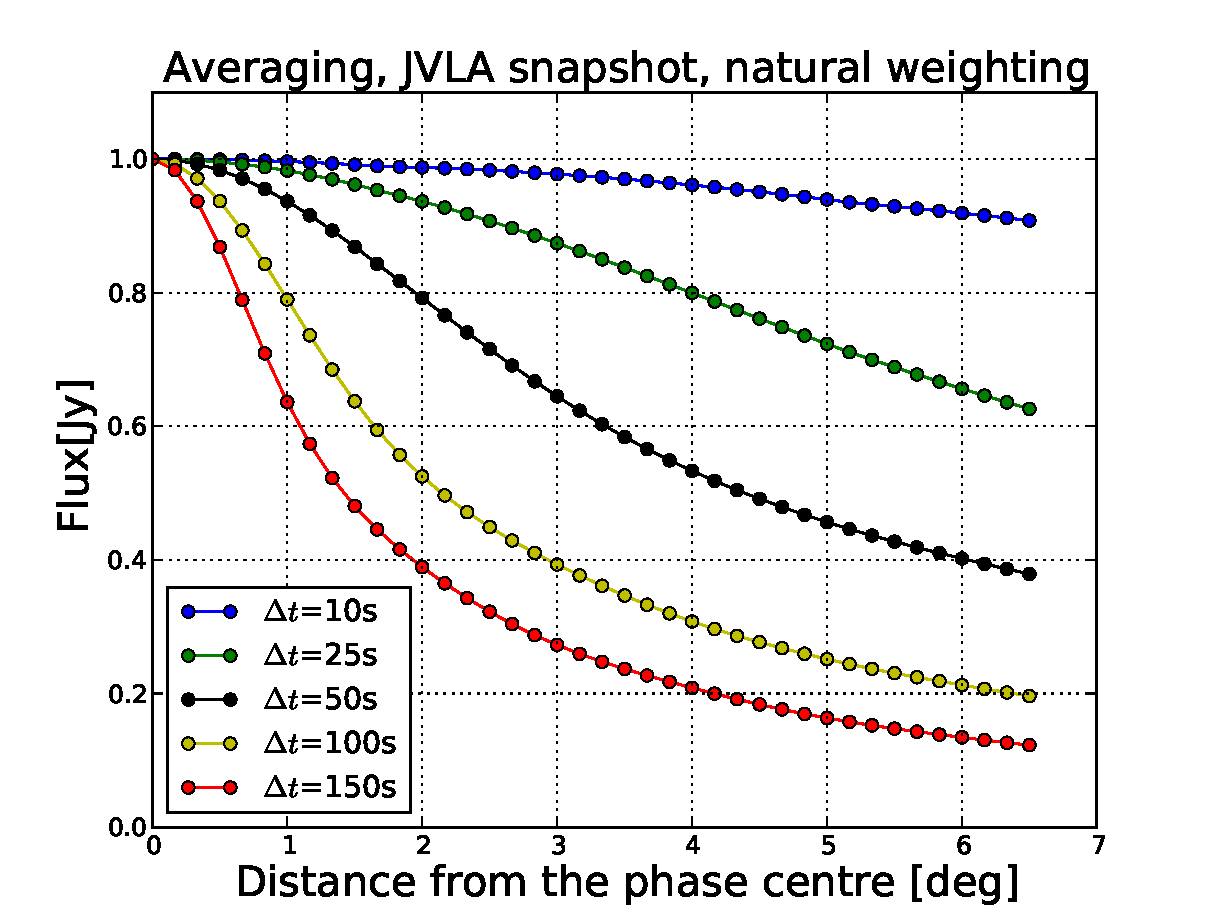
\includegraphics[width=1\textwidth]{./Figures/effect_time_averaging.pdf}\caption{Attenuation of the 
intensity of a 1Jy source move from the phase centre for $\Delta t$ integration synthesis at $1.4$GHz with
125kHz bandwidth.}\label{timessear1}\end{minipage}
\hspace{1cm}
\begin{minipage}{0.38\linewidth}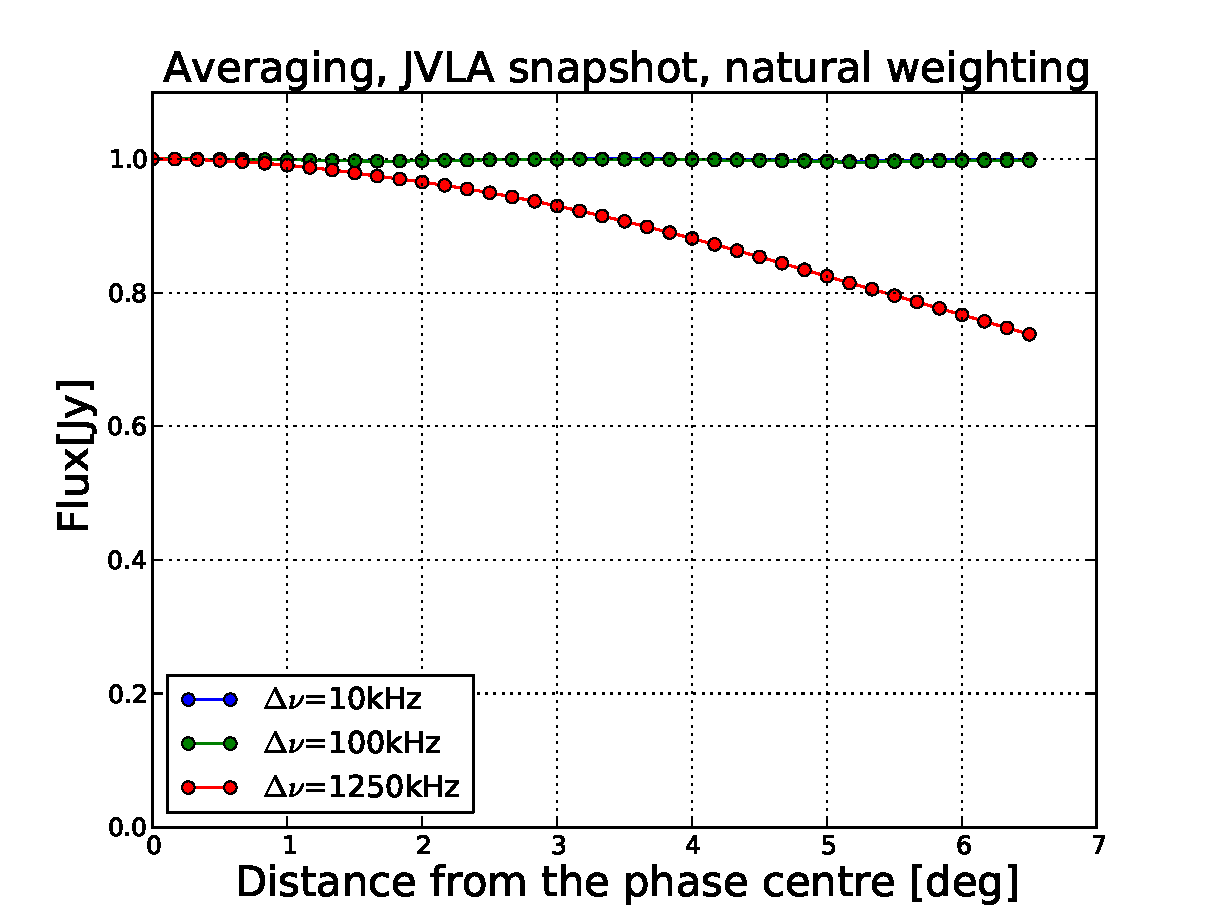
\includegraphics[width=1\textwidth]{./Figures/effect_bandwid_averaging.pdf}\caption{Attenuation of the 
intensity of a 1Jy source move from the phase centre for $1$s integration synthesis at $1.4$GHz with
$\Delta \nu$ bandwidth.}\label{timessear2}\end{minipage}
\end{figure*}
\subsection{Imaging}
\label{sec:imaging}
Recall from the previous section that, the boxcar windowing function can be replaced by a windowing function, $W_{pq,(t,\nu)}$ that depends 
on $(u,v)$ spacing. Now, consider that $\mathcal{\textbf{W}}_{pq,(t,\nu)}$ is a $n_t \times n_{\nu}$ matrix of elements 
$W_{pq,(t_i,\nu_j)}|_{i=1,n_t}^{j=1, n_{\nu}}$, the weights of $(u,v)$ points. From the full sky Radio Interferometry Measurement Equation 
(RIME) formalism \citep{smirnov2011revisiting}, \citep{smirnov2011revisiting}, the sampled visibilities can be presented mathematically as 
a $4\times 
n_t\times n_{\nu}$ matrix of four polarization times and 
frequencies dependent matrices each of size $n_t\times n_{\nu}$.
\begin{eqnarray*}
\mathbf{V}_{pq,(t,\nu)}^{samp}&=&\Bigg(\mathbf{V}_{pq,(t,\nu)}^{0},\mathbf { V } 
^1_{pq,(t,\nu)},\mathbf{V}^2_{pq,(t,\nu)},\mathbf{V}_{pq,(t,\nu)}^{3 } \Bigg)^{\dagger}, \label{eqx:conv}
\end{eqnarray*}
where the symbol $^{\dagger}$ stand for the transpose operation. The convolution operator is linear, therefore we can re-write Eq.\ref{f4} 
in terms of a series of linear transformations or functional models as:
\begin{equation}
V_{pq,(t_c,\nu_c)}^{corr}= \mathbf{C}_{pq,(t,\nu)}^{block}\cdot\mathbf{W}_{pq,(t,\nu)}^{block}\cdot 
\mathbf{V}_{pq,(t,\nu)}^{samp}.\label{eqbb:linear}
\end{equation}
Here, $\mathbf{C}_{pq,(t,\nu)}^{block}$ and $\mathbf{W}_{pq,(t,\nu)}^{block}$ are  blocks diagonals matrices of size $(4n_t 
n_{\nu})\times(4n_t n_{\nu})$, the block elements are $\mathcal{\textbf{W}}_{pq,(t,\nu)}$ and $\mathbf{C}_{pq,(t,\nu)}$ 
respectively, where $\mathbf{C}_{pq,(t,\nu)}$ is the centre time interval and centre frequency interval sampling matrix of size $n_t\times 
n_{\nu}$. This
is the result of the time and frequency integration for the baseline $(p,q)$.
For a synthesis, the baseline $(p,q)$ made a full coverage in the $(u,v)$ plane. Therefore, we can  
package into a single matrix, $\mathbf{V}_{pq,(t',\nu')}^{corr}$ of size $(4N_t N_{\nu})\times (4N_t N_{\nu})$ the 
weighted average visibilities of the  baseline $(p,q)$ during the synthesis as follows: 
\begin{equation}
\mathbf{V}_{pq,(t',\nu')}^{corr}=\mathbf{C}_{pq,(t,\nu)}^{block,n}\cdot 
\mathbf{W}_{pq,(t,\nu)}^{block,n}\cdot\mathbf{V}_{pq,(t,\nu)}^{samp,n},\label{eq2:block}
\end{equation}
where $N_t$ and  $N_{\nu}$ are the number of time sample and frequency channels entering the Fourier domain. If the synthesis time is $T$ 
and the frequency range is $F$, then $T=N_t \times \Delta t$ and $F=N_{\nu}\times\Delta \nu$. The the size of 
$\mathbf{V}_{pq,(t',\nu')}^{corr}$ can also be written as $(4N_v^{pq})\times (4N_v^{pq})$, where $N_v^{pq}$ is the 
number of time and frequency visibilities for the baseline $(p,q)$. The matrices
$\mathbf{C}_{pq,(t,\nu)}^{block,n}$ and $\mathbf{W}_{pq,(t,\nu)}^{block,n}$ are diagonals blocks 
matrices of size $(4N_v^{pq}n_t n_{\nu})\times (4N_v^{pq}n_t n_{\nu})$ where each diagonal block is the block diagonal matrix  
$\mathbf{C}_{pq,(t,\nu)}^{block}$ and $\mathbf{W}_{pq,(t,\nu)}^{block}$ respectively. $n$ is the number of blocks 
elements. The sampled  visibilities 
$\textbf{V}_{pq,(t,\nu)}^{samp,n}=\mathcal{\textbf{S}}_{pq,(t,\nu)}^{n}\cdot\mathbf{V}_{pq,(t,\nu)}^{n}$ is a one row matrix of size 
$(N_v^{pq}4 n_t n_{\nu})\times (4 n_t n_{\nu})$ made of $\textbf{V}_{pq,(t,\nu)}^{samp}$ on top of each other and the matrix 
$\mathcal{\textbf{S}}_{pq,(t,\nu)}^{n}$ is the $(u,v)$ plane sampling function for the visibilities $\mathbf{V}_{pq,(t,\nu)}^{n}$ of size  
$(N_v^{pq}4 n_t n_{\nu})\times (4 n_t n_{\nu})$. We can write:
\begin{equation}
\mathbf{V}_{pq,(t' \nu')}^{corr}= 
\mathbf{C}_{pq,(t,\nu)}^{block,n}\cdot\mathbf{W}_{pq,(t,\nu)}^{block,n}\cdot 
\mathbf{S}_{pq,(t,\nu)}^{n}\mathbf{F}\cdot\mathcal{I}_{l,m}^{sky },\label{eqv:linear}
\end{equation}
if the number of pixel in the sky model is $N_{pix}$, then the true sky image vector $\mathcal{I}_{l,m}^{sky}$ has a size of $4N_{pix}$ and 
$\textbf{F}$ is a block diagonal Fourier transform operator of size $(4N_{pix})\times(4N_{pix})$. 

We are generally interested in using the total set of visibilities over baselines, time and frequencies, having $4\times N_v$ visibilities 
measured over all baselines  and $N_v=n_{bl}\times N_v^{pq}$ in this case. Here, $n_{bl}$ is the number of baseline. We then have:
\begin{equation}
 \mathbf{V}_{array,(t',\nu')}^{corr}=\mathbf{A}\cdot\mathcal{I}_{l,m}^{sky} + \epsilon. \label{eq:vall}
\end{equation}
Our data is always corrupted by a random error component or noise, $\epsilon$   and $\mathbf{A}$ is the design matrix of size 
$(4N_v)\times (4N_{pix})$ 
corresponding to $N_v$ visibilities weights, defined as
\begin{equation*}
\mathbf{A}_{}=
  \begin{bmatrix}
    \mathbf{C}_{(t,\nu)}^{block,n}\cdot \mathbf{W}_{01,(t,\nu)}^{block,n}\cdot \mathbf{S}_{01,(t,\nu)}^{n} \cdot\mathbf{F}\\
    \vdots\\
    \mathbf{C}_{(t,\nu)}^{block,n}\cdot \mathbf{W}_{ik,(t,\nu)}^{block,n}\cdot \mathbf{S}_{ik,(t,\nu)}^{n} \cdot\mathbf{F}\\
    \vdots \\
    \mathbf{C}_{(t,\nu)}^{block,n}\cdot \mathbf{W}_{jl,(t,\nu)}^{block,n}\cdot \mathbf{S}_{jl,(t,\nu)}^{n} \cdot\mathbf{F}\\
  \end{bmatrix}
\end{equation*}
The dirty image, $\mathcal{I}_{l,m}^{D}$ of size $4N_{pix}$ can then be derived as follow:
\begin{equation}
\mathcal{I}_{l,m}^{D}=\mathbf{F}^{H}\cdot\mathbf{A}\cdot\mathcal{I}_{l,m}^{sky} + \epsilon.
\end{equation}
Here, $H$ represents the the conjugate transpose operation also known as a Hermitian transpose and $\mathbf{F}^{H}$ is a block diagonal
inverse Fourier transform operator of size $(4N_{pix})\times(4N_{pix})$. The estimate of  $\epsilon$, for the map centre pixel is given by:
\begin{eqnarray*}
 \widetilde{\epsilon}_{o,o}&=&\widetilde{\mathcal{I}}_{o,o} - \mathbf{F}^{H}\cdot\mathbf{A}\cdot\widetilde{\mathcal{I}}_{o,o}
\end{eqnarray*}
\begin{eqnarray}
	&=&\frac{1}{N_{v}}\sum_{k=1}^{N_{v}^{pq}}\Bigg\{\mathbf{B}\cdot\mathbf{V}_{array,(t,\nu)}^{n}-
\mathbf{F}^{H}{H}\cdot\mathbf{A}\cdot\mathbf{B}\cdot\mathbf{V}_{array,(t,\nu)}^{n}\Bigg\} \label{eq:noise}
\end{eqnarray}
Here, $\mathbf{B}$ and $\mathbf{V}_{array,(t,\nu)}^{n}$ are  one row matrix of size $(N_v 4 n_t n_{\nu})\times (4 n_t n_{\nu})$ made of 
$\mathbf{C}_{(t,\nu)}^{block,n}\cdot \mathbf{W}_{01,(t,\nu)}^{block,n}\cdot \mathbf{S}_{01,(t,\nu)}^{n}$ and $\mathbf{V}_{pq,(t,\nu)}^{n}$
on top of each other respectively (see appendix \ref{app:complexmatrices} for the derivation of these complex matrices).
\section{Algorithm 1: FoV signals recovery}
\label{baseline1}
\subsection{Description}
Missing spaces between sampled $(u,v)$ coordinates has an important dependence on the baseline length. However, the spacings between longer 
baselines $(u,v)$ coordinates are wider than the one on shorter baselines, this is the obvious effect that explained why sources are more 
distorted on longer baselines compared to shorter ones. Therefore, if one have to attribute a $(u,v)$ weight, it may be as a function of 
the baseline length, in such a way that the distortion rate is taken into account over baselines. We aimed in this section, to 
describe an algorithm that we used with a  windowing function to assign a proper weight to a data reference by a $(u,v)$ 
coordinate considering the \textit{spacing}\footnote{The \textit{distance} also has huge 
dependences on the baseline length and allows us to formally define the data
weight of a $uv$ point over the entire $uv$ plane.} between the baseline $(u,v)$ coordinates.

Fig.\ref{fig:uvcov} shows a snapshot coverage of an integration interval. For shorter baselines, the tracks are closer to the centre of 
rotation and for longer baselines the tracks are farther away from this centre. The \textit{dot marks} are the data for a sampled $(u,v)$ 
data, and the  arrows indicates the separation between $(u,v)$ coordinates and the centre $(u,v)$ coordinates. It is trivial to see on this 
figure that these separations are wider on longer baselines. The results of averaging is assigned to the centre $(u,v)$ coordinates 
coloured 
in red. 
\subsection{Methods}
\label{sec:baseline1}
Depending on the arrays, we show
here that we can use the fact that, the spacings of long baselines $(u,v)$ coordinates are wider and  
design a high dynamic range filter on longer baselines that will recover the desire FoV of the interferometer, and at the same time 
reducing the data rate. During an integration, the Earth rotation makes baselines coordinates $u$ and $v$  to vary in time and 
frequency. We can therefore package the $(u,v)$ coordinates changes and the frequency changes of a baseline $pq$ into a single matrix of 
size $n_t \times 2$ and  into a single vector of dimension $n_{\nu}$ respectively. 
\begin{eqnarray*}
\mathbf{U}_{pq,t}&=& \Bigg(\mathbf{u}_{pq,t_s}, \dots , \mathbf{u}_{pq,t_c}, \dots, \mathbf{u}_{pq,t_e}\Bigg)^{\dagger}\\
 \mbox{\boldmath $\nu$}&=&\Bigg(\nu_s,\dots,\nu_c,\dots,\nu_e\Bigg)^{\dagger}
\end{eqnarray*}
where the indexes $s$, $c$ and $e$ references the integration interval starting, centre, and ending time respectively. 
The 
elements of $\mathbf{U}_{pq,t}$ are functions of time and frequency representing a $(u,v)$ coordinate.
We defined the function, $\overline{\overline{\cdot}}$ on a $n_t \times 2$ matrix as follow:
\begin{eqnarray}
\overline{\overline{\mathbf{U}}}_{pq,t}=\Bigg(||\mathbf{u}_{pq,t_s}||, \dots , ||\mathbf{u}_{pq,t_c}||, \dots, 
||\mathbf{u}_{pq,t_e}||\Bigg)^{\dagger},
\end{eqnarray}
where $||.||$ is the Euclidean norm.
\begin{definition}[Time direction spacing]
\label{def:1}
The matrix that models the spacing between the $(u,v)$ coordinates and the centre $(u,v)$ coordinate of a baseline $(p,q)$ across the time 
direction is defined as
\begin{eqnarray*}
 \mathbf{U}_{pq,t}^{s} &=&\frac{\nu_c}{c}\cdot\Bigg\{\mathbf{U}_{pq,t}-\mathbf{H}_{pq,t} \Bigg \},
\end{eqnarray*}
where $c$ is the speed of the light and $\mathbf{H}_{pq}$ is a matrix of size $n_t \times 2$ that models the centre $uv$-coordinate,
$\mathbf{H}_{pq,t}= \big(\mathbf{u}_{pq,t_c}, \dots , \mathbf{u}_{pq,t_c}, \dots, \mathbf{u}_{pq,t_c}\big)^{\dagger}$.
\end{definition}
\begin{definition}[Frequency direction spacing]
\label{def:2}
The vector of size $n_{\nu}$ that model the spacing between the $(u,v)$ coordinates and the centre $(u,v)$ coordinate of a baseline $(p,q)$ 
across the frequency direction is defined as
\begin{eqnarray*}
\mathbf{d}^{}_{\nu} &=&\frac{||\textbf{u}_{pq,t_c}||}{c}\cdot\Bigg\{\mbox{\boldmath 
$\nu$}-\nu_c\cdot\mathbf{g}_{\nu} \Bigg \},
\end{eqnarray*}
where  $\textbf{g}$ is a $n_{\nu}\times1$ unity matrix. The weight of a $(u,v)$ data point is considered as follow:
\end{definition}
\begin{definition}[Baseline dependent windowing function]
\label{def:3}
If $f_{pq}$ is a \textit{baseline dependent windowing function}, then:
\begin{eqnarray*}
 f_{pq}: \{\mathbf{\mathcal{R}},\mathbf{\mathcal{R}}\} &\rightarrow& \mathbf{\mathcal{R}}\\
                   d_{t_i},d_{\nu_j} &\mapsto& \frac{w_{t_i,\nu_j}}{\sum_{i=1}^{n_t}\sum_{j=1}^{n_{\nu}}w_{t_i,\nu_j}}.
\end{eqnarray*}
where $d_{t_i}$ is an element of the vector $\mathbf{d}_{t}=\overline{\overline{\mathbf{U}^{s}}}_{pq,t}$ and $d_{\nu_j}$ is an element 
of the vector $\mathbf{d}^{}_{\nu}$.
\end{definition}
The previous algorithm is correct. But unfortunately, the algorithm did not suppress out FoV sources and we lost  in sensitivity. 
Although simple averaging "means high sensitivity", we do need to eliminate at a certain rate out FoV sources in such a way that the 
overall SNR becomes higher than the one of averaging. We described such an algorithm in the following section.
\begin{figure}
  \centering
    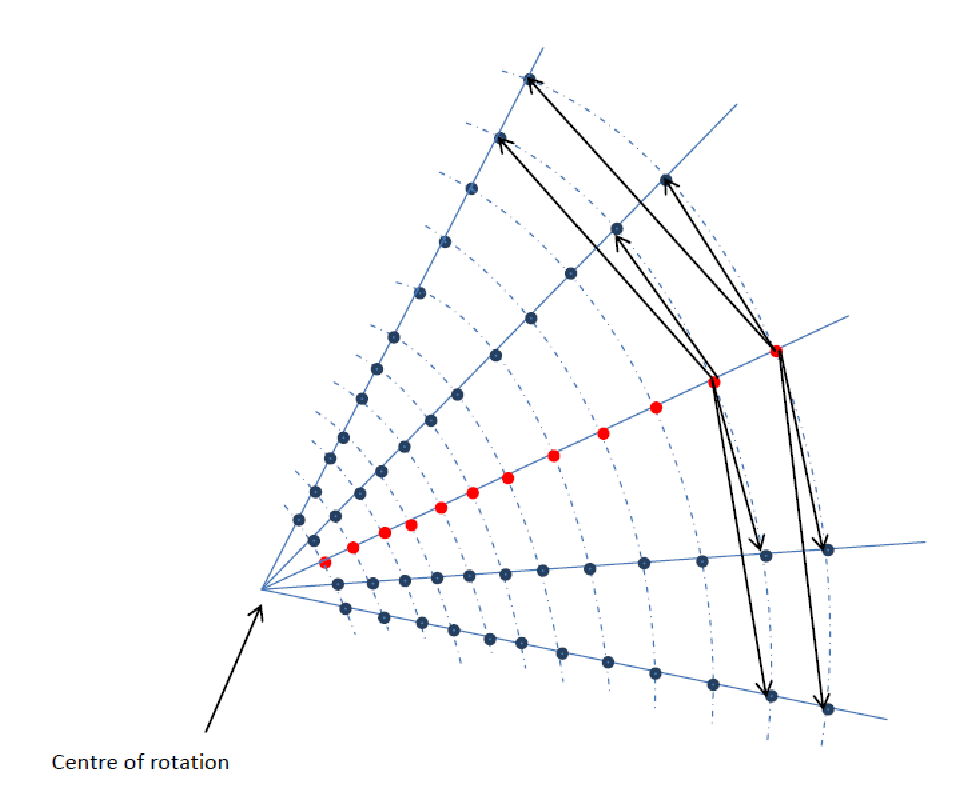
\includegraphics[width=0.5\textwidth]{./Figures/uvcov.png}
    \caption{Coverage of one integration}\label{fig:uvcov}
\end{figure}
\section{Algorithm 2: FoV signals recovery and out FoV suppression}
\label{baseline2}
\subsection{Description}
In theory, windowing functions and signals generally extend to  infinity. Unfortunately, in practice, filtering a signal with a low pass 
filter, one need to define a cut-off interval. Therefore, if one  wants to achieve sufficiently an accurate  estimate of the 
windowing function ideal spectrum, one need a wide cut-off interval as far as the spectrum approaches the ideal when the windowing function 
order increases. An overlap baseline dependent windowing function aims to extend the order of the baseline dependent windowing function in 
such a way that, we approach the ideal spectrum.
%, but by maintaining the same cut-off interval like the boxcar one. 
The only drawback of this technique is the increase in time needed for processing the output sample of the signals being integrate.  
\subsection{Methods}
The weight of a visibility is not defined by a unique baseline dependent windowing, but by the strength of the correlation between the 
overall  overlapping baseline dependent windowing functions on the visibility. Now, consider that $f^{a}_{pq}$ is an overlap-\textit{BDWF} 
of width  $\Delta t$ and $\Delta \nu$ across the time and frequency direction respectively.
\begin{definition}[Left hand side overlapping functions]
\label{def:4}
if $\Delta_l t$ and $\Delta_l \nu$ are the overlap time interval and frequency interval of the baseline dependent windowing function  
$f_{pq}^{a_0}$ respectively  and $\Big\{f_{pq}^{a_1},f_{pq}^{a_2},f_{pq}^{a_3}, \dots \Big\}$ the set of \textit{BDWF} overlapping  on the 
\textit{left hand side} of $f_{pq}^{a_0}$ then the resulting \textit{BDWF} within $\Delta_l t$ and $\Delta_l \nu$ is defined as
\begin{eqnarray*}
 g^{lhs}_{pq}: \{\mathbf{\mathcal{R}},\mathbf{\mathcal{R}}\} &\rightarrow& \mathbf{\mathcal{R}}\\
                   d_{t_i},d_{\nu_j} &\mapsto& \frac{1}{N_{lhs}}\Bigg(\sum_{k}f_{pq,(d_{t_i},d_{\nu_j})}^{a_k} 
+ f_{pq,(d_{t_i},d_{\nu_j})}^{a_0}\Bigg).
\end{eqnarray*}
Here, $N_{lhs}$ is the normalization term defined as
\begin{eqnarray*}
N_{lhs}=\sum_{i=1}^{n_{lt}}\sum_{j=1}^{n_{l\nu}}\Bigg(\sum_{k}f_{pq,(d_{t_i},d_{\nu_j})}^{a_k} + f_{pq,(d_{t_i},d_{\nu_j})}^{a_0} \Bigg),
\end{eqnarray*}
where $n_{lt}$ and $n_{l\nu}$ are the number of $(u,v)$ coordinates changes and frequency changes  within $\Delta_l t$ and $\Delta_l \nu$ 
respectively.
\end{definition}
\begin{definition}[Right hand side overlapping functions]
 \label{def:4}
 if $\Delta_r t$ and $\Delta_r \nu$ are the overlap time and frequency interval of a \textit{BDWF} $f_{pq}^{a_0}$ 
respectively and  $\Big\{f_{pq}^{a_1},f_{pq}^{a_2},f_{pq}^{a_3}, \dots \Big\}$ the set of \textit{BDWF} overlapping on the \textit{right 
hand side} of $f_{pq}^{a_0}$, then the 
resulting \textit{BDWF} within $\Delta_r t$ and $\Delta_r \nu$ is defined as
\begin{eqnarray*}
 g^{rhs}_{pq}: \{\mathbf{\mathcal{R}},\mathbf{\mathcal{R}}\} &\rightarrow& \mathbf{\mathcal{R}}\\
                   d_{t_i},d_{\nu_j} &\mapsto& 
\frac{1}{N_{rhs}}\Bigg (f_{pq,(d_{t_i},d_{\nu_j})}^{a_0}+\sum_{k}f_{pq,(d_{t_i},d_{\nu_j})}^{a_k}\Bigg ).
\end{eqnarray*}
Here, $N_{rhs}$ is the normalization term defined as
\begin{eqnarray*}
N_{rhs}=\sum_{i=1}^{n_{rt}}\sum_{j=1}^{n_{r\nu}}\Bigg(f_{pq,(d_{t_i},d_{\nu_j})}^{a_0} + \sum_{k}f_{pq,(d_{t_i},d_{\nu_j})}^{a_k}\Bigg),
\end{eqnarray*}
where $n_{rt}$ and $n_{r\nu}$ are the number of $(u,v)$ coordinates changes and frequency changes  within $\Delta_r t$ and $\Delta_r \nu$ 
respectively.
\end{definition}
\begin{definition}[Overlap baseline dependent windowing functions]
 \label{def:4}
If $f_{pq}^{a_0}$ is a baseline dependent windowing function defined within the time interval $\Delta t$ and the frequency interval 
$\Delta \nu$, $g^{lhs}_{pq}$ the result of the left hand side of $f_{pq}^{a_0}$ overlapping windowing functions within the time interval 
$\Delta_l t$ and the frequency interval $\Delta_l \nu$, and $g^{rhs}_{pq}$  the result of the right hand side of $f_{pq}^{a_0}$ overlapping 
windowing functions within the time interval $\Delta_r t$ and the frequency interval 
$\Delta_r \nu$, then the overlap baseline dependent windowing function within  $\Delta t$ and $\Delta \nu$ is defined as:
\begin{eqnarray*}
 g^{}_{pq}: \{\mathbf{\mathcal{R}},\mathbf{\mathcal{R}}\} &\rightarrow& \mathbf{\mathcal{R}}\\
                   d_{t_i},d_{\nu_j} &\mapsto&
 \left\{ 
  \begin{array}{l l}
    g^{lhs}_{pq} & \quad \text{if $(t_i,\nu_j) \in (\Delta_l t, \Delta_l \nu)$}\\
    f^{a_0}_{pq} & \quad \text{if $(t_i,\nu_j) \in (\Delta_m t, \Delta_m \nu)$}\\
    g^{rhs}_{pq}& \quad \text{if $(t_i,\nu_j) \in (\Delta_r t, \Delta_r \nu)$}
  \end{array} \right.
\end{eqnarray*}
\end{definition}
where $\Delta_m t$ and $\Delta_m \nu$ are $f_{pq}^{a_0}$ uncorrelated time  and frequency interval respectively. From the above 
definitions, the following derivation is trivial 
\begin{equation*}
 \Big\{\Delta t,\hspace{0.17cm}\Delta \nu \Big\}=\Big\{\Delta_l t \cup \Delta_m t \cup \Delta_r t, \hspace{0.17cm}\Delta_l \nu \cup 
\Delta_m \nu \cup \Delta_r \nu \Big\}.
\end{equation*}
 They follow the rules below:
\begin{eqnarray*}
 \Delta_m t= \left\{ 
  \begin{array}{l l}
     \cup\{t_i\}_{i=s',\hspace{0.1cm} s' \geq s+1}^{e', \hspace{0.1cm}e'\leq e-1} & \quad \text{if $n_{lt}+n_{rt}< n_t$}\\
      \{t_c\}& \quad \text{if $n_{lt}+n_{rt} = n_t$}\\
       \emptyset  & \quad \text{otherwise}
  \end{array} \right.
\end{eqnarray*}
and
\begin{eqnarray*}
 \Delta_m \nu= \left\{ 
  \begin{array}{l l}
     \cup\{\nu_i\}_{i=s',\hspace{0.1cm} s'\geq s+1}^{e', \hspace{0.1cm}e'\leq e-1} & \quad \text{if $n_{l\nu}+n_{r\nu} < n_{\nu}$}\\
      \{\nu_c\}& \quad \text{if $n_{l\nu}+n_{r\nu} = n_{\nu}$}\\
       \emptyset  & \quad \text{otherwise}
  \end{array} \right.
\end{eqnarray*}
\subsection{Windowing functions}
\label{subsec:Windowing functions}
In signal processing a windowing function is a mathematical function that has zero-values outside some chosen interval, and when a signal 
is multiplied by the windowing function, the product has also zero-values outside the interval.
In this section, we evaluate the Peak Sidelobe Level (PSL), the Main 
Lobe width (MLW) and the Sidelobes Roll-off (SLR) for some windowing functions spectrum. The goal of this study is to find a windowing 
function that its spectral response  will conserved the signal within a field of interest while suppressing sidelobes confusion from strong 
sources outside the field of interest.\\
In the table below, we present the terminology that will be using in this paper in contrast of the terminology used in signal 
processing.\\ 
\begin{tabular}{*3{c}}\\
 \multicolumn{3}{|c|}{}
 \hspace{-1cm}\begin{tabular}{|l|l|l|l|}
  \hspace{3cm}\footnotesize Table of terms \\
  \hline
  \footnotesize Signal processing &\footnotesize BDWFs\\
  \hline\hline
  {\footnotesize Frequency (freq) domain} &{\footnotesize Image plane} \\
  {\footnotesize Time domain} &{\footnotesize Fourier plane}\\
  {\footnotesize Spectral response or freq response} & {\footnotesize Image taper}\\
  {\footnotesize Cut-off time interval or time pass band} &{\footnotesize $\Delta t$ and/or $\Delta \nu$}\\
  {\footnotesize Cut-off freq interval or freq pass band} &{\footnotesize FoV}\\
  {\footnotesize Time stop band} &{\footnotesize Outside $\Delta t$ and/or $\Delta \nu$}\\
  {\footnotesize Freq stop band} &{\footnotesize Outside edges of FoV}\\
  \end{tabular}
\end{tabular}
\subsubsection{Boxcar window}
The Boxcar window is a function that  conserved a constant non-zero value  inside a chosen  interval and zero value outside this interval.
When a signal is cut-off with this window, this leads to discontinuities at the edges\footnote{unless its 
happens that the signal  fit exactly with the window width. Nevertheless, it is rare to find such a situation.}. For 
a cut-off time interval  $[-t_a,t_a]$ the boxcar window is defined as:
\begin{equation}
\Pi(t)=\left\{
\begin{array}{rl}
1 & \mbox{$-t_a \leq t \leq t_a$} \\
0 & \mbox{otherwise}
\end{array}\right.
\end{equation}
Fig.\ref{fig:fig_box} and Fig.\ref{fig:fig_box_freq} give the graph of $\Pi(t)$ and its spectrum respectively. The blue and 
the red curves of Fig.\ref{fig:fig_box_freq} are the spectrum of $\Pi(t)$ for a time cut-off interval, $[-t_a, t_a]$ and 
$[-t_a/2,t_a/2]$ respectively. Note that when the cut-off interval is large, the MLW of the spectrum is 
narrower, the PSL is lower and the SLR drops faster.
\subsubsection{Gaussian window}
A Gaussian window centred at mean zero with standard deviation $\sigma$ is given by: 
\begin{equation}
  G(t)= e^{-bt^{2}}, \label{eq:gauss}
\end{equation}
where, $b=(2\sigma^2)^{-1}$. The inverse Fourier transform of Eq.\ref{eq:gauss} is given by 
$\mathcal{F}^{-1}\big\{G(t)\big\}=\sqrt{\frac{b}{\pi}}e^{-cl^2}$, where $c=\pi^2/b$.
This shows us that the inverse Fourier transform of a Gaussian with standard deviation $\sigma$ is a Gaussian with a standard 
deviation $\sigma '= (2\pi\sigma)^{-1}$.
Fig.\ref{fig:fig_gauss} and Fig.\ref{fig:fig_gauss_freq} give the graph of $G(t)$ and its spectrum respectively, where $G(t)$ 
is truncated within the cut-off frequency interval $[-t_a,t_a]$, with $b = 3$ for the blue curve and $b=5$ for the red curve. Note 
that when the standard deviation is large, the MLW of the spectrum is narrower, the PSL is higher and the SLR drops slowly compared to a 
smaller standard deviation.
\subsubsection{Butterworth window}
The time response of the Butterworth window is flat  in the pass band, and rolls off towards zero in the stop band, and it is 
characterized by two independent parameters, the cut-off time $t_a$ and the order $p$. These two parameters control the 
bandwidth and sidelobes  attenuation. The time response of the Butterworth window is given by:
\begin{equation}
BW(t)= \Big(1 + (t/t_a)^{2p}\Big)^{-1}.
\end{equation}
For the same frequency interval $[-t_a,t_a]$ we plotted  three curves $\{p=1, p=3, p=5\}$ of $BW(t)$ in Fig.\ref{fig:fig_butter} and 
their corresponding spectrum in Fig.\ref{fig:fig_butter_freq}. Note that when the order $p$ increases, the MLW of the 
spectrum is conserved, while the PSL also increase and the SLR drops faster.
\subsubsection{Sinc Window}
The sinc window is defined as follow:
\begin{equation}
S(t)= sinc\big(\pi b t\big).
\end{equation}
 Fig.\ref{fig:fig_sinc} and Fig.\ref{fig:fig_sinc_freq} gives the graph of $S(t)$ and its spectrum respectively, where 
$S(t)$ is truncated within the cut-off time interval $[-t_a,t_a]$. Note that when the cut-off time interval is large 
(Fig.\ref{fig:fig_sinc_freq}, blue curve), the spectrum becomes perfectly flat at the pass band while the MLW becomes narrower,  the PSL 
becomes lower and the SLR drops faster compared to a cut-off interval of $[-t_a/2,t_a/2]$ (Fig.\ref{fig:fig_sinc_freq}, red curve). 
\subsubsection{Bessel Function of the First Kind of order zero}
 This function can  be determined using the infinity power series expansion:
\begin{equation}
J_0(t) = \sum_{k=0}^{\infty}\frac{(-1)^k (x/2)^{2k}}{(k!)^2}
\end{equation}
 Fig.\ref{fig:bessel} and Fig.\ref{fig:freq_resp_bessel} gives the graph of J$_0(t)$ and its spectrum respectively, where 
J$_0(t)$ is truncated within the cut-off time interval $[-t_a,t_a]$. Note that when the cut-off time interval is large 
(Fig.\ref{fig:freq_resp_bessel}, blue curve), the spectrum is flat at the pass band while the MLW becomes narrower,  the PSL 
becomes lower and the SLR drops faster compared to a cut-off interval of $[-t_a/2,t_a/2]$ (Fig.\ref{fig:freq_resp_bessel}, red curve).\\
 The table below summarizes the MLW, the PSL and the SLR of the windows taken under consideration in this section.
\begin{tabular}{*3{c}}
 \multicolumn{3}{|c|}{}\\
 \begin{tabular}{|l|l|l|l|}
  \footnotesize Windows &\textbf{\footnotesize MLL (-3db)}&\textbf{\footnotesize PSL (db)} &\textbf{\footnotesize SLR (db/octave) }  \\
  \hline\hline
  {\footnotesize $\Pi(t)$} &{\footnotesize $\approx 0,073$} &{\footnotesize $-6,68$}&{\footnotesize $-6,78$}\\
  {\footnotesize $S(t)$} &{\footnotesize  $\approx0,306$}&{\footnotesize  $-11,22$}&{\footnotesize  $-12,42$} \\
  {\footnotesize $G(t)$} & {\footnotesize $\approx0,0736$}&{\footnotesize  $-30,28$}&{\footnotesize  $-14,5$}\\ 
  {\footnotesize $BW(t)$} &{\footnotesize  $\approx0,079$} &{\footnotesize $-10,08$ }&{\footnotesize  $-15,39$}\\
  {\footnotesize $J_0(t)$} &{\footnotesize  $\approx 0,39$} &{\footnotesize $ -15,01$ }&{\footnotesize  $ -14,01$}
  \end{tabular}& \label{BDWBnoise}
\end{tabular}\\
A windowing function with a narrower main lobe width (for a better spectral resolution), lowers PSL (to achieve less
masking of nearby sources), and faster SLR (to achieve less masking for far away sources) is preferably in this work.
\begin{figure*}
  \centering
  \begin{minipage}{0.36\linewidth}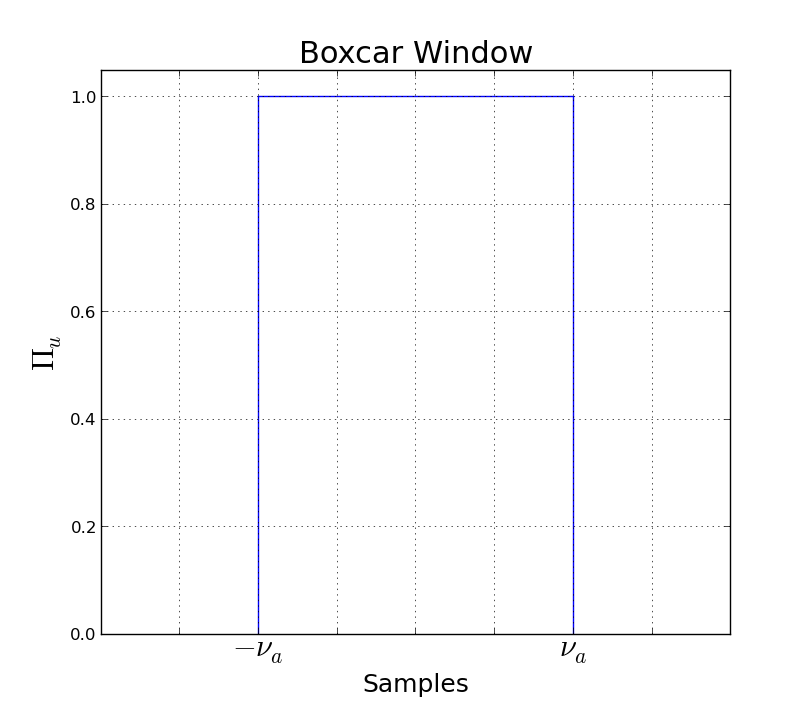
\includegraphics[width=1\textwidth]{./Figures/rect.png}\caption{Boxcar windowing 
function.}\label{fig:fig_box}\end{minipage}
\hspace{1cm}
\begin{minipage}{0.36\linewidth}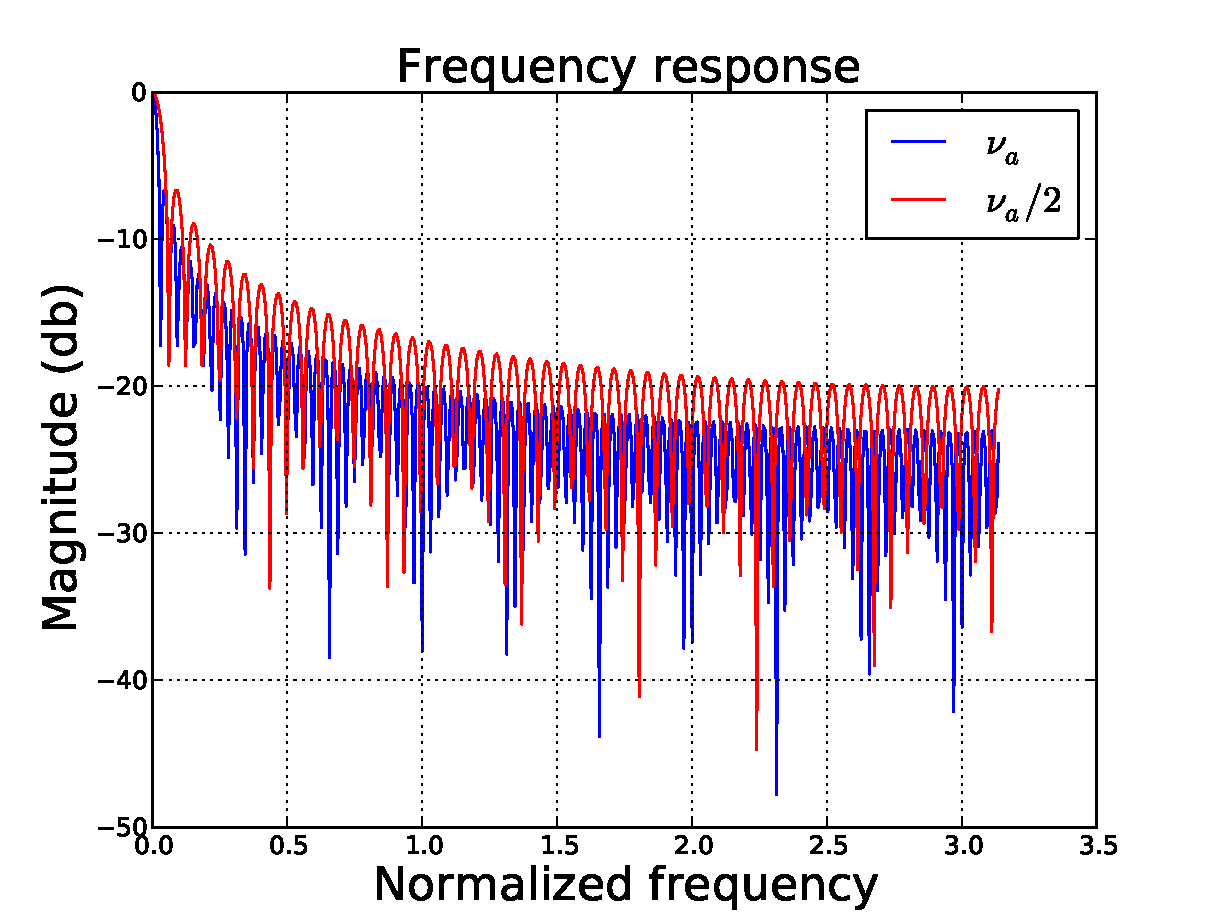
\includegraphics[width=1\textwidth]{./Figures/freq_resp_box.pdf}\caption{Frequency response of a boxcar 
window}\label{fig:fig_box_freq}\end{minipage}\\
\begin{minipage}{0.36\linewidth}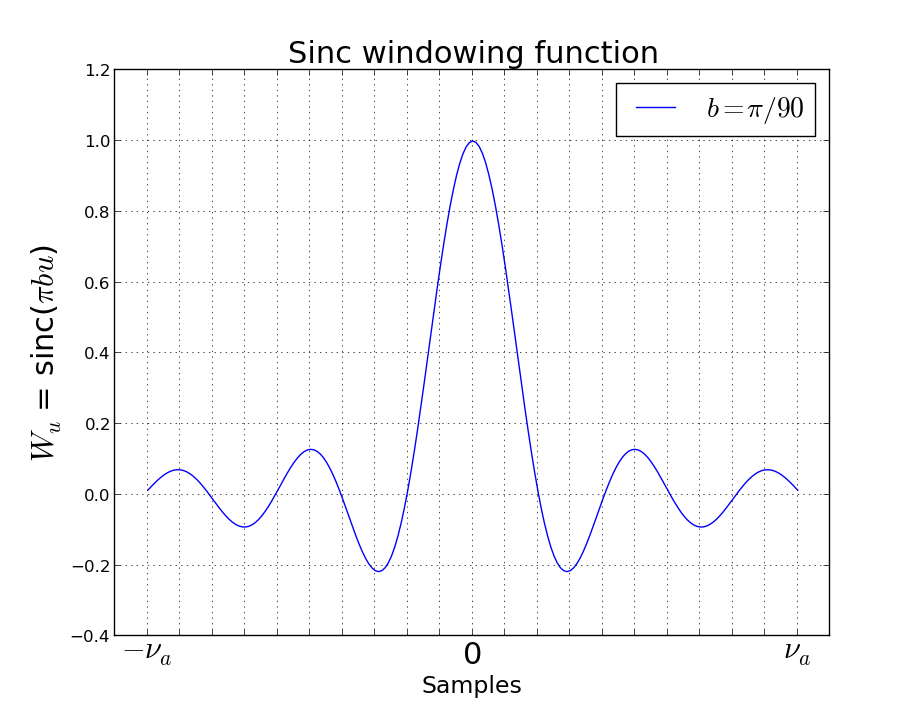
\includegraphics[width=1\textwidth]{./Figures/sinc.png}\caption{Sinc 
window}\label{fig:fig_sinc}\end{minipage}
\hspace{1cm}
\begin{minipage}{0.36\linewidth}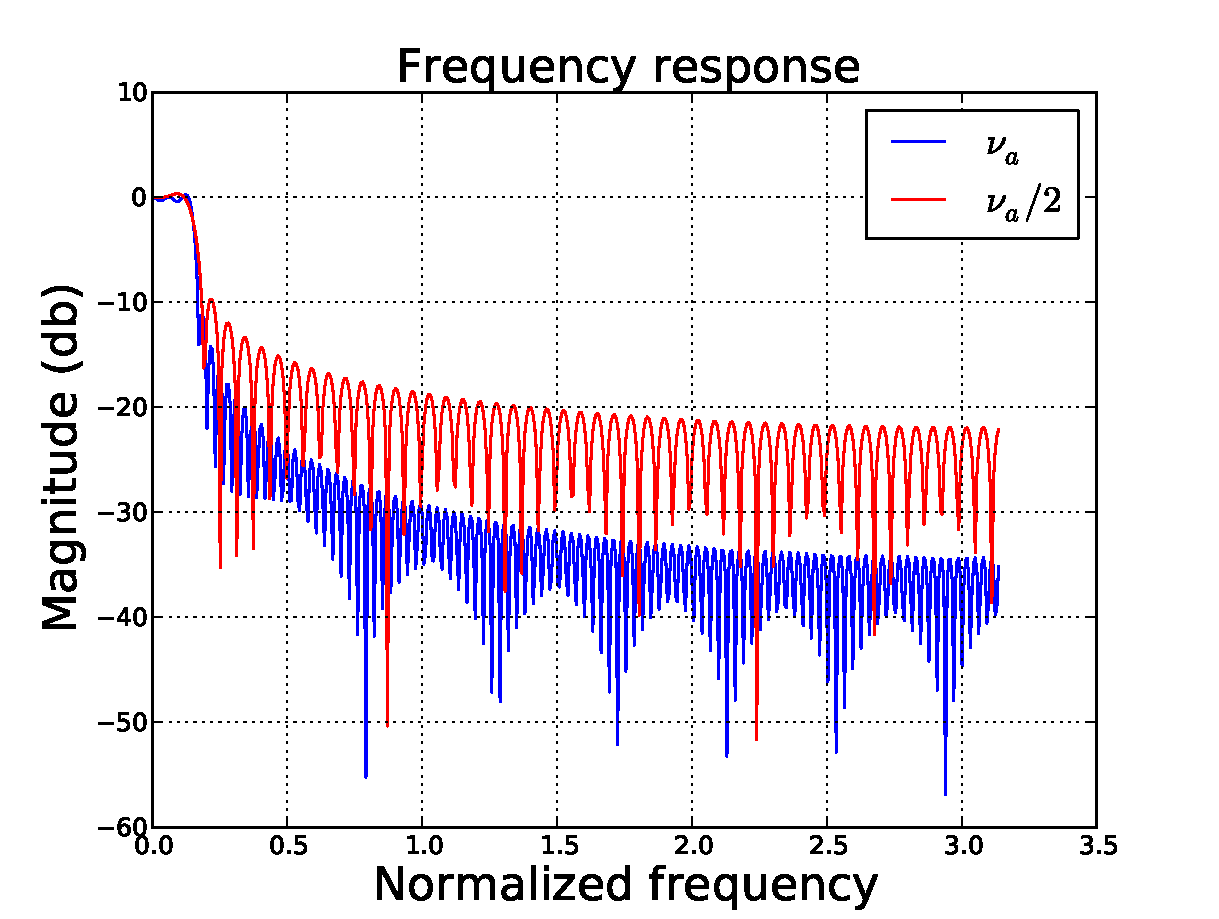
\includegraphics[width=1\textwidth]{./Figures/freq_resp_sinc.pdf}\caption{Frequency response of the 
sinc window }\label{fig:fig_sinc_freq}\end{minipage}\\
\begin{minipage}{0.36\linewidth}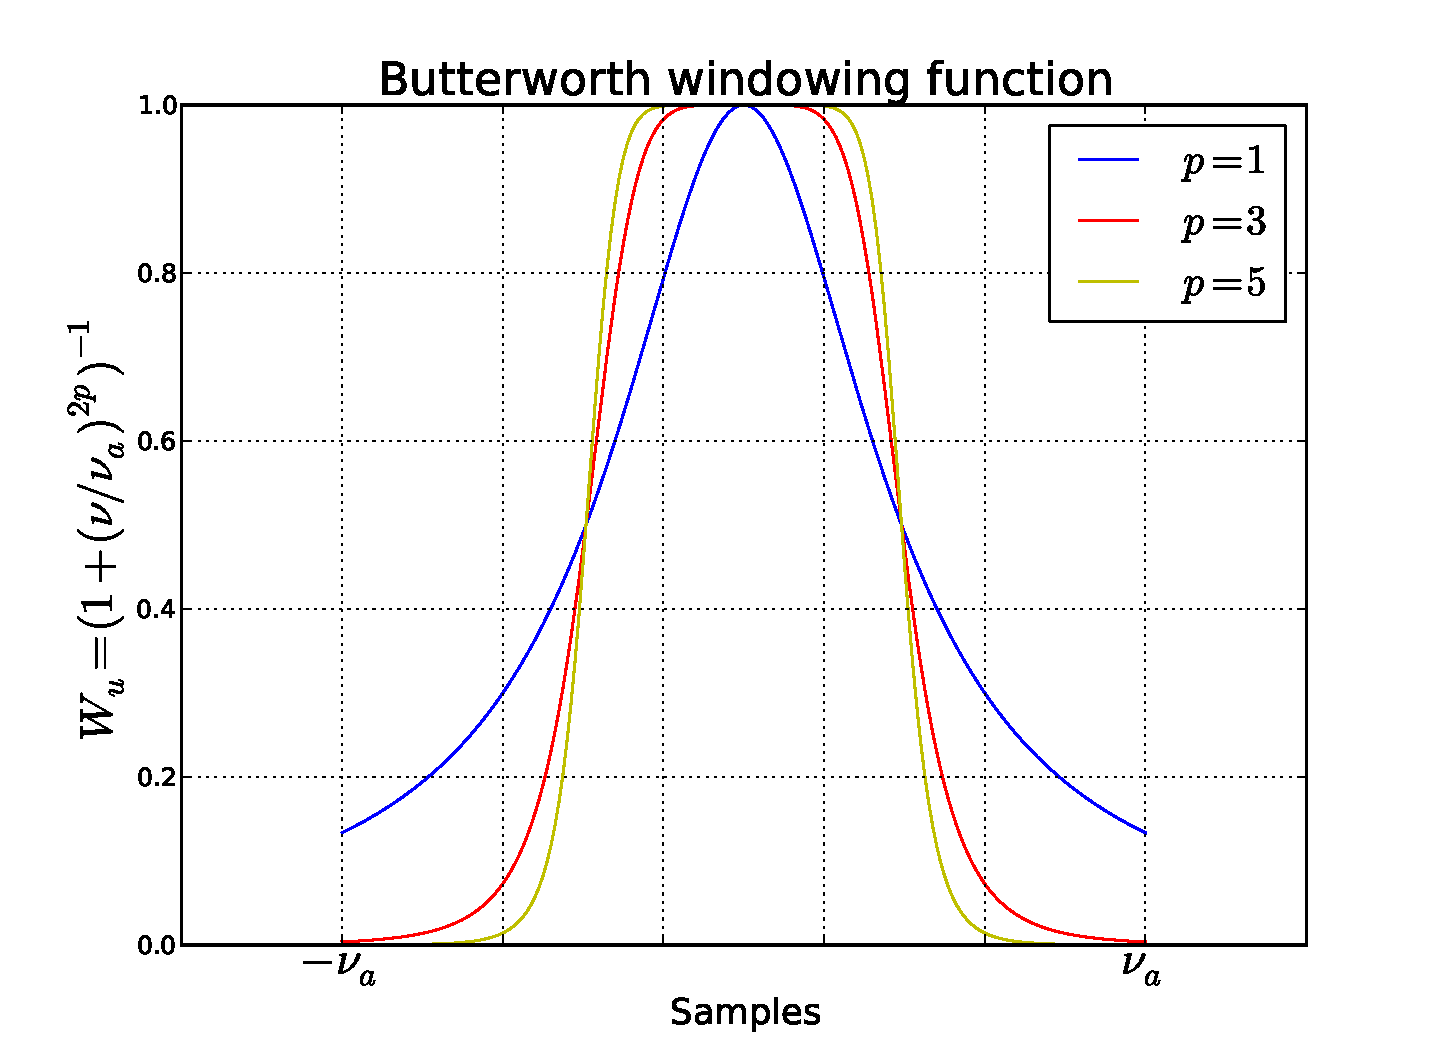
\includegraphics[width=1\textwidth]{./Figures/Butterwordth.pdf}\caption{ Butterwordth 
windows}\label{fig:fig_butter}\end{minipage}
\hspace{1cm}
\begin{minipage}{0.36\linewidth}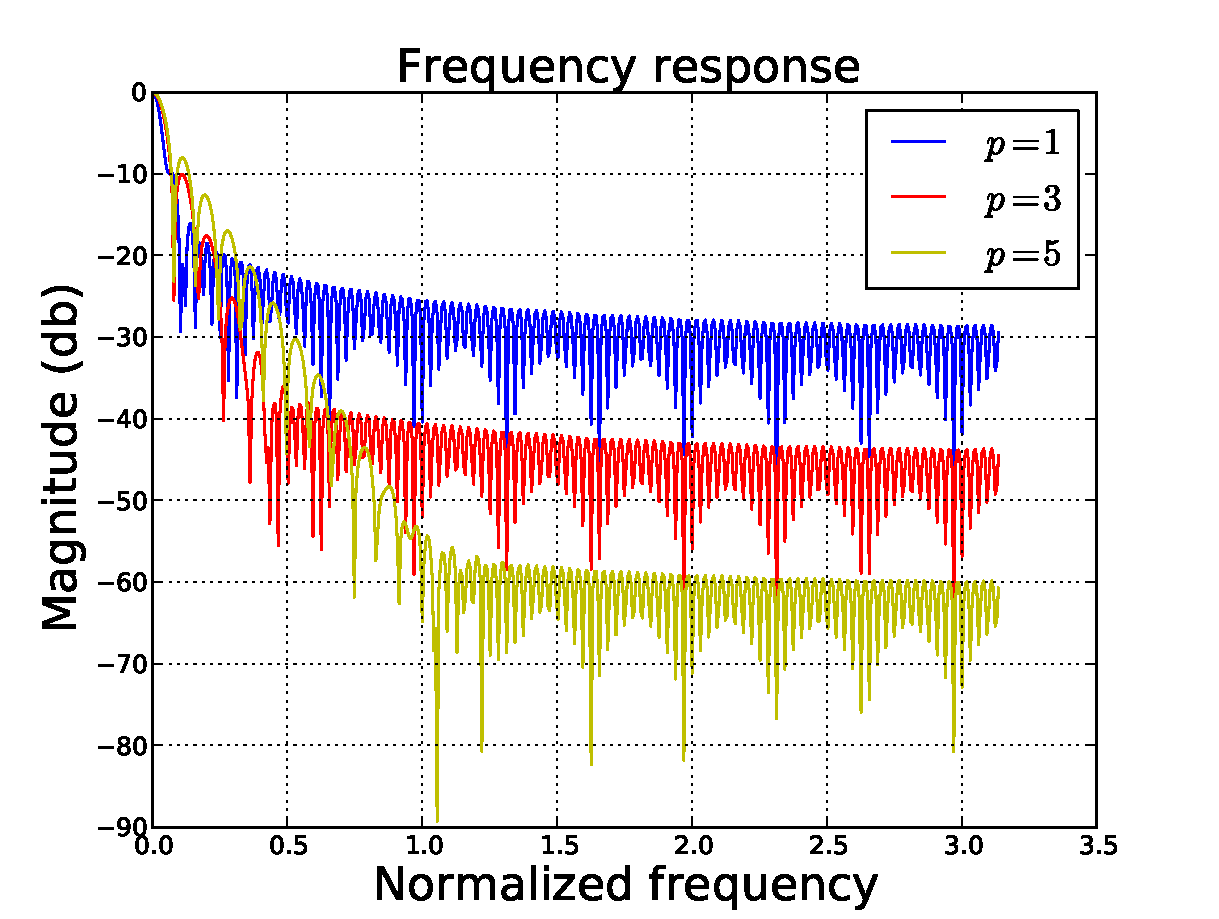
\includegraphics[width=1\textwidth]{./Figures/freq_resp_butterwordh.pdf}\caption{Frequency response 
of the Butterwordth windows}\label{fig:fig_butter_freq}\end{minipage}\\
\begin{minipage}{0.36\linewidth}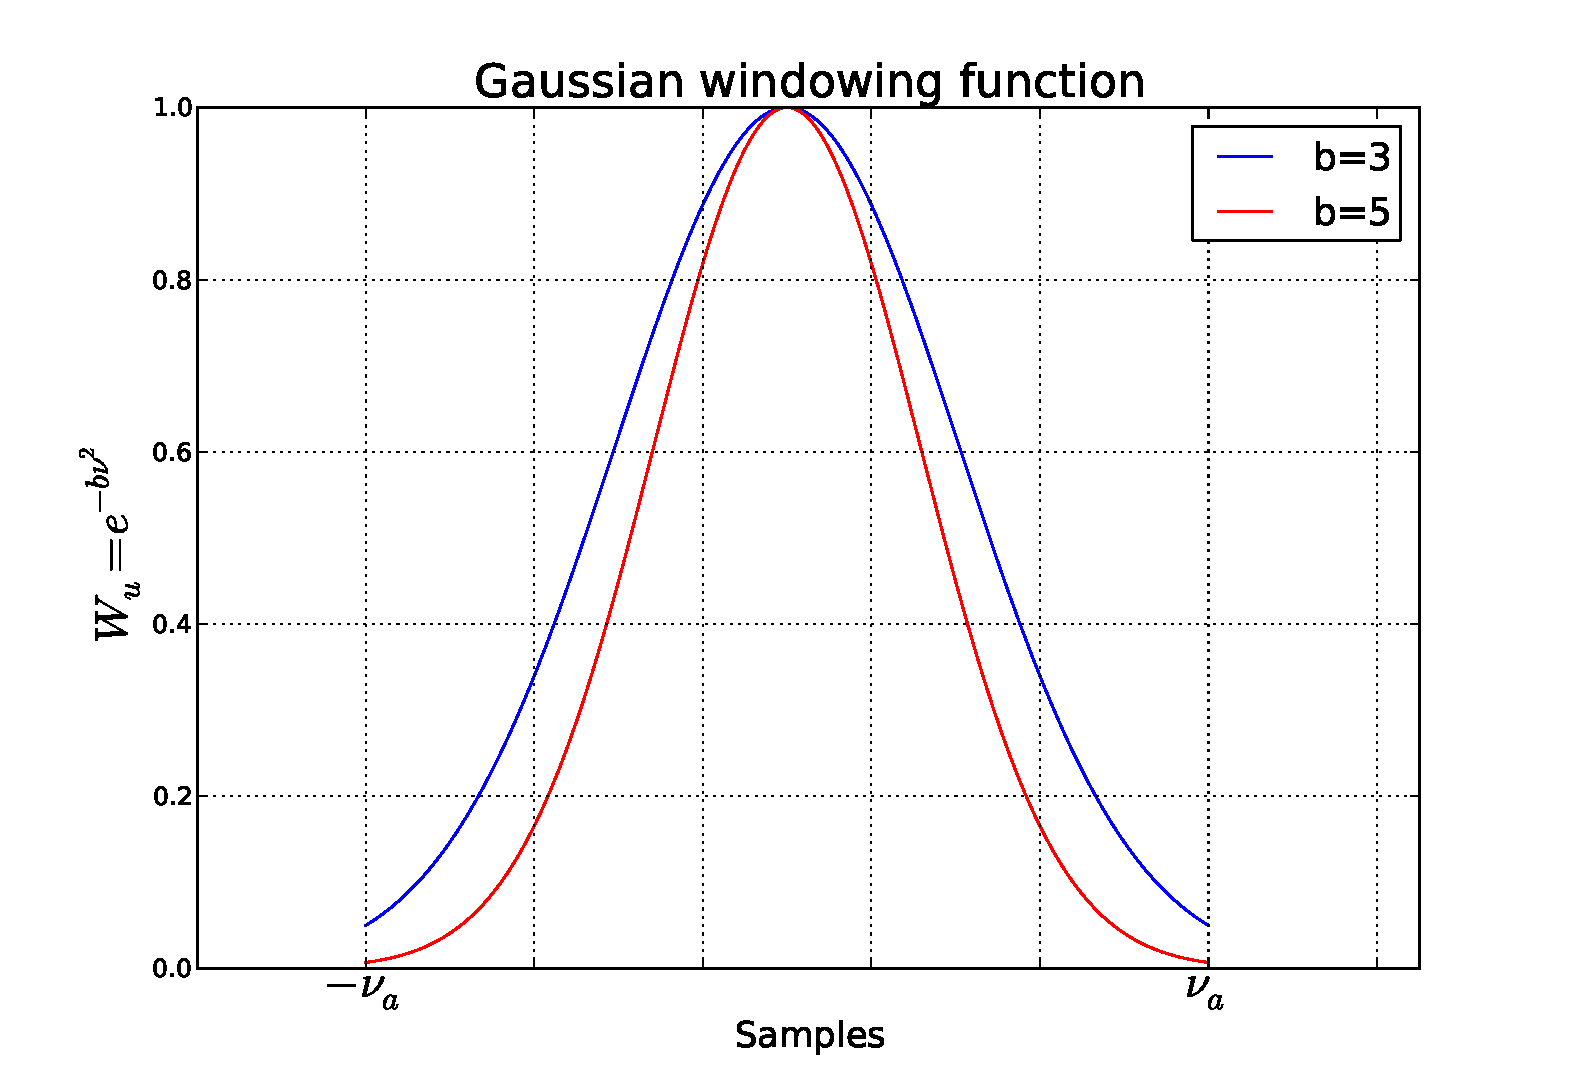
\includegraphics[width=1\textwidth]{./Figures/gausian.pdf}\caption{Gaussian windows}\label{fig:fig_gauss}
\end{minipage}
\hspace{1cm}
\begin{minipage}{0.36\linewidth}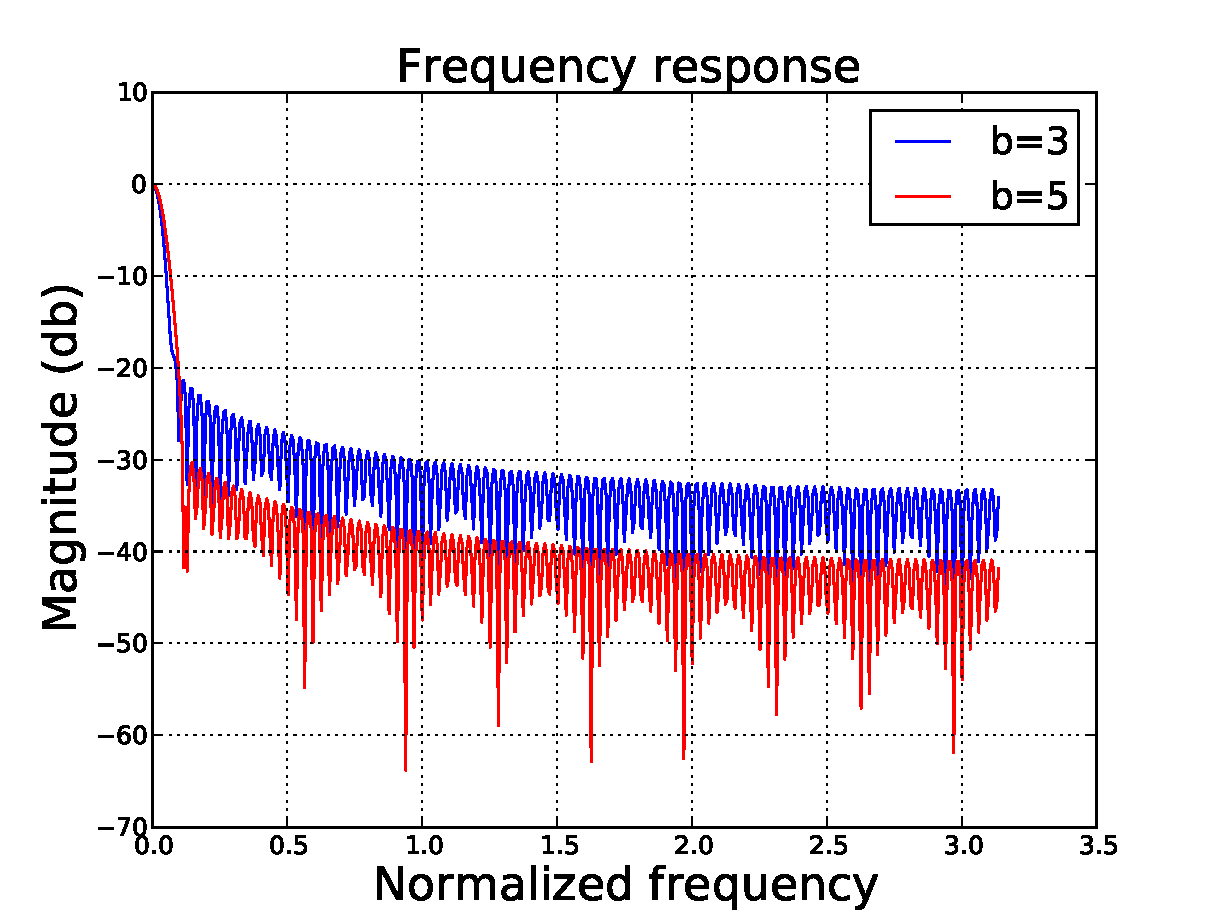
\includegraphics[width=1\textwidth]{./Figures/freq_resp_gaussian.pdf}\caption{Frequency response of 
Gaussian windows}\label{ fig:fig_gauss_freq } \end{minipage}
\end{figure*}
\begin{figure*}
  \centering
\begin{minipage}{0.36\linewidth}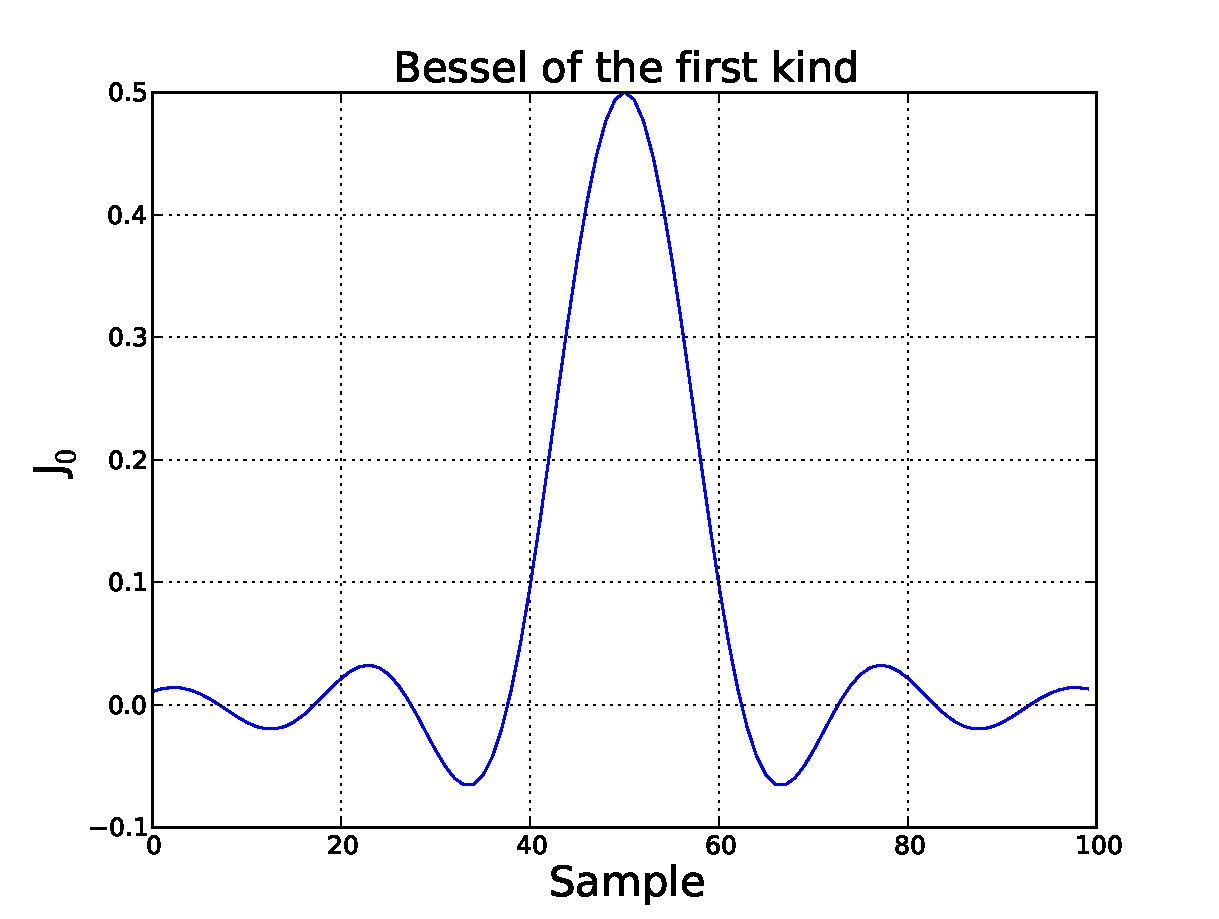
\includegraphics[width=1\textwidth]{./Figures/bessel.pdf}\caption{Bessel 
first King windows NB: this figure is coming very soon}\label{fig:bessel}\end{minipage}
\hspace{1cm}
\begin{minipage}{0.36\linewidth}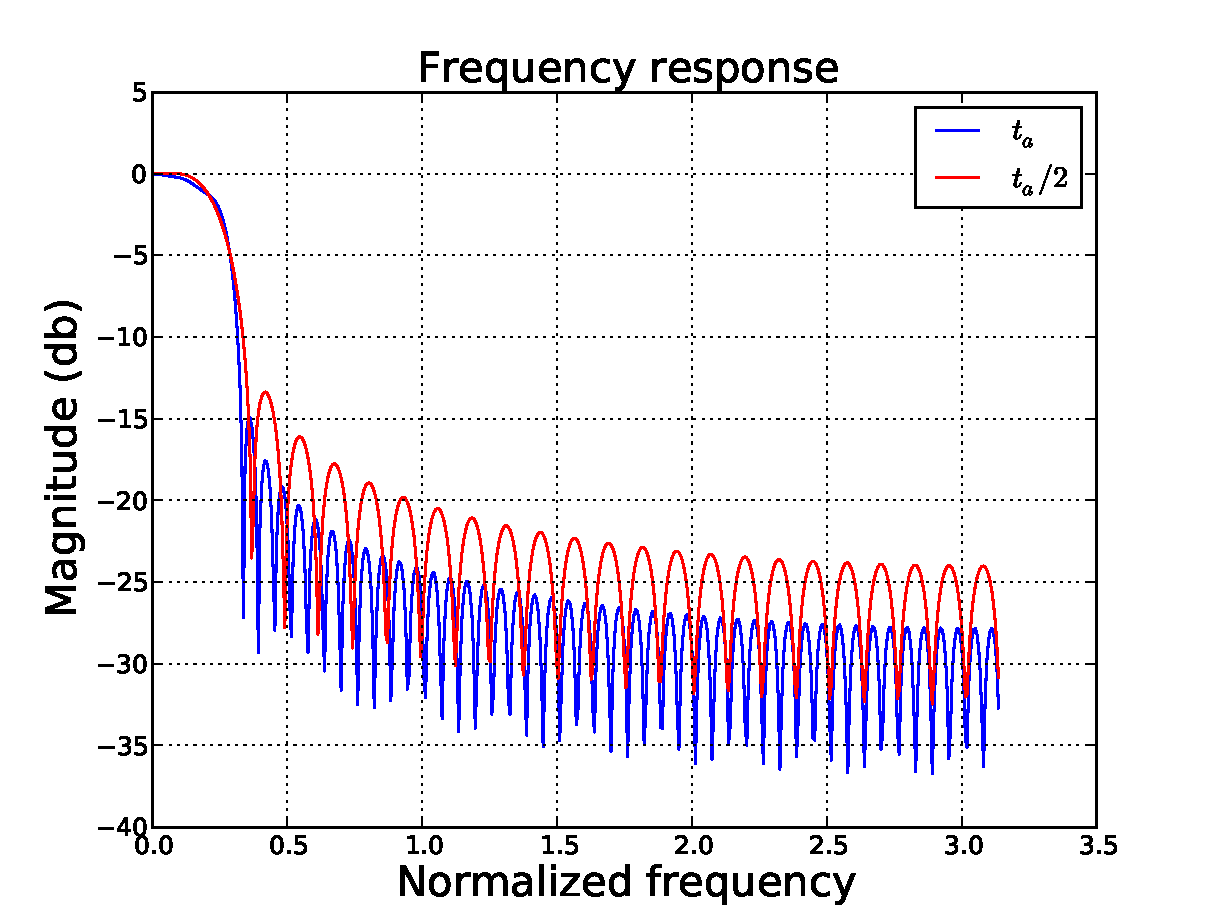
\includegraphics[width=1\textwidth]{./Figures/freq_resp_bessel.pdf}\caption{Frequency 
response of Bessel first kind window}\label{fig:freq_resp_bessel} \end {minipage}
\end{figure*}
\section{Noise and comparison}
Several windowing functions  were described in the previous section, however in the rest of this paper we only consider the sinc 
window, the Bessel of the first kind and the Butterwordth.  We considered 
$sinc(X,Y)=sinc(X)sinc(Y)$, J$_0(X,Y)=$J$_0(\sqrt{X^2 + Y^2})$ and $BW(X,Y)=BW(\sqrt{X^2 + Y^2})$ for a two dimensional 
sinc window, Bessel of the first kind and Butterwordth window respectively. We show in this section that on shorter baselines, the 
windowing functions reduce to the Boxcar window. Therefore, we effectively applying a hybrid filter; a Boxcar on the shorter baselines and 
the given windowing function on the longer baselines (see Fig.\ref{fig:longshortmid-sinc}, Fig.\ref{fig:longshortmid-bessel} and 
Fig.\ref{fig:longshortmid-butter}). We furthermore show the behaviour of an overlap baseline dependent windowing function 
in Fig.\ref{fig:corrSigVLAMxBl_overlapLdelta}, Fig.\ref{fig:corrSigVLAMxBl} and Fig.\ref{fig:corrSigVLAMxBl_overlapGdelta} and evaluate the 
theoretical noise predicted in 
Eq.\ref{eq:noise} (see \ref{fig:per-baseline-noise-ratio-sinc}, Fig.\ref{fig:per-baseline-noise-ratio-bessel} 
and \ref{fig:per-baseline-noise-ratio-BW}).
\begin{figure*}
 \centering
  \begin{minipage}{0.38\linewidth}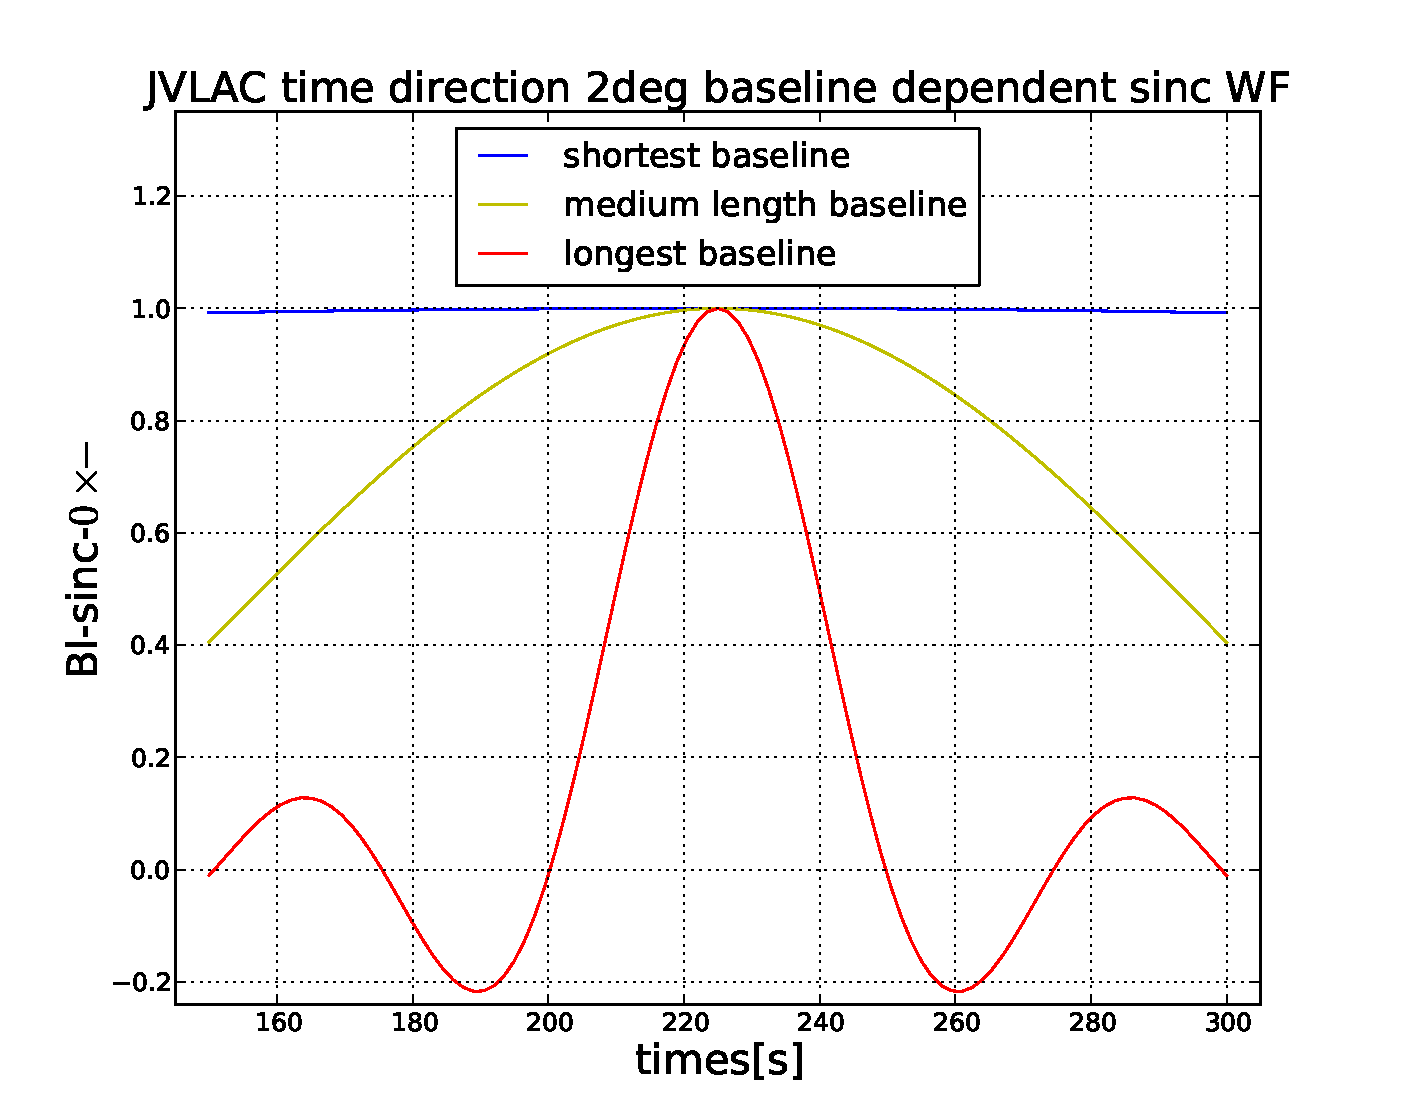
\includegraphics[width=1\textwidth]{./Figures/longshortmid-sinc.pdf}
  \caption{Time direction Bl-sinc-W0 of the shortest, medium and longest baseline}\label{fig:longshortmid-sinc}
  \end{minipage}
  \hspace{1cm}
  \begin{minipage}{0.38\linewidth}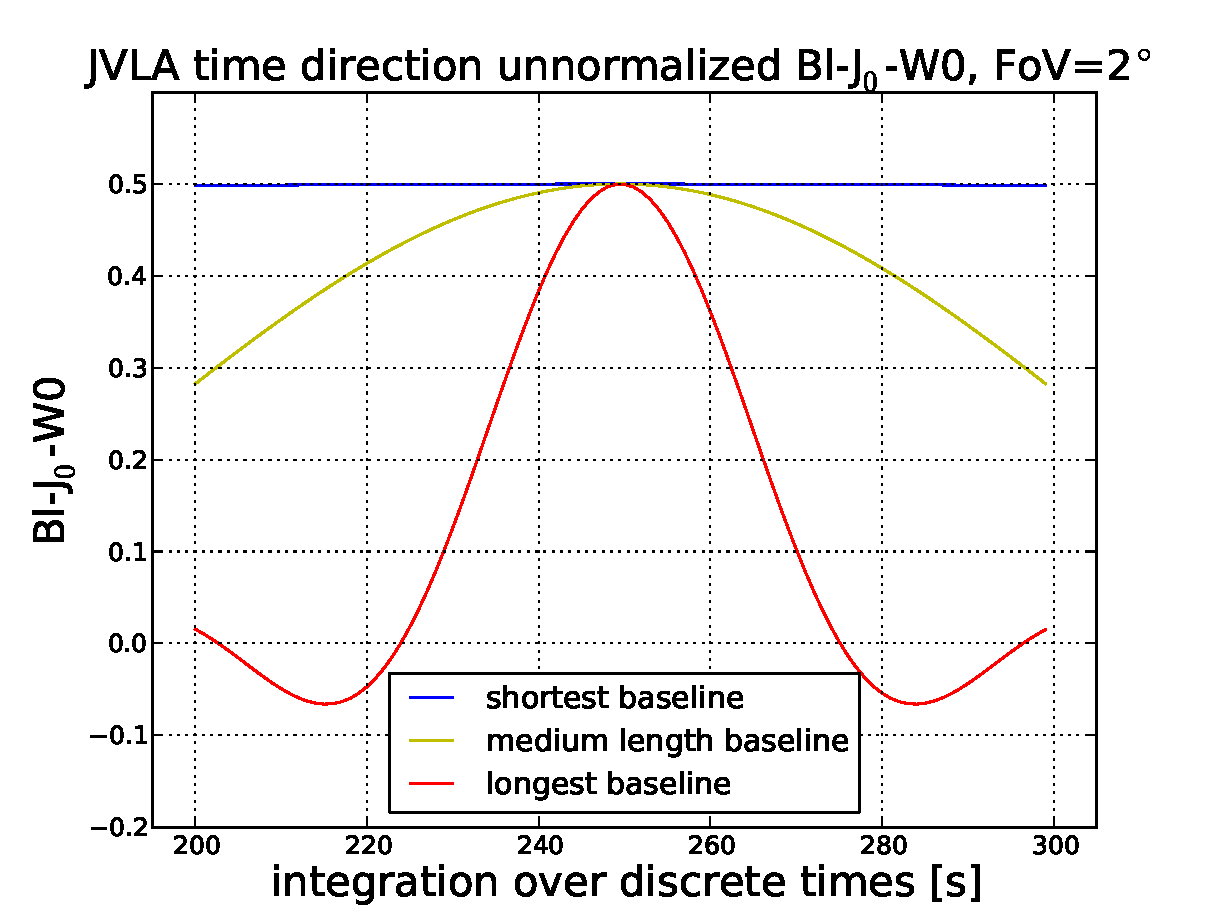
\includegraphics[width=1\textwidth]{./Figures/longshortmid-bessel.pdf}
  \caption{Time direction Bl-J$_0$-W0 of the shortest, medium and longest baseline}\label{fig:longshortmid-bessel}
  \end{minipage}\\
  \begin{minipage}{0.38\linewidth}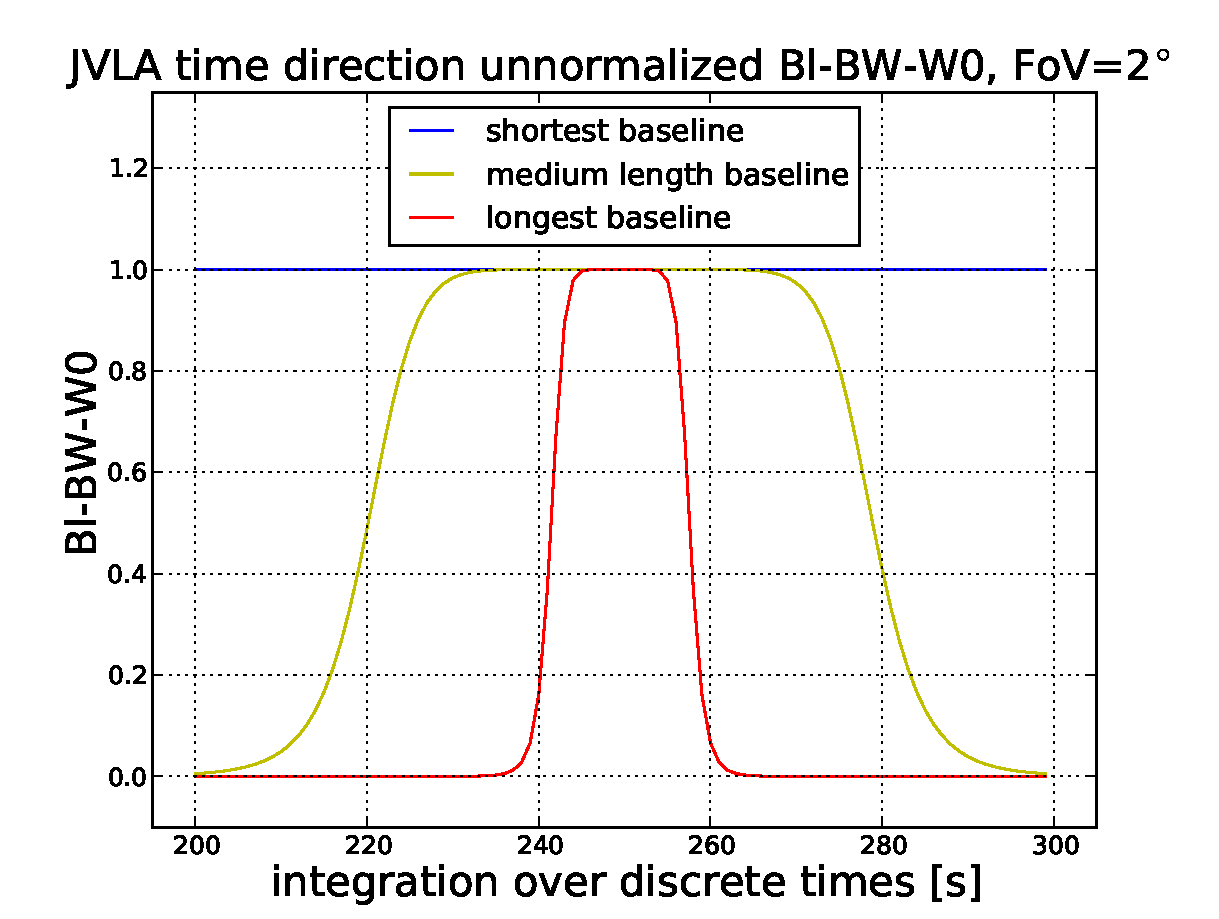
\includegraphics[width=1\textwidth]{./Figures/longshortmid-butter.pdf}\\
  \caption{Time direction Bl-BW-W0 of the shortest, medium and longest baseline}\label{fig:longshortmid-butter}
  \end{minipage}
  \hspace{1cm}
\begin{minipage}{0.38\linewidth}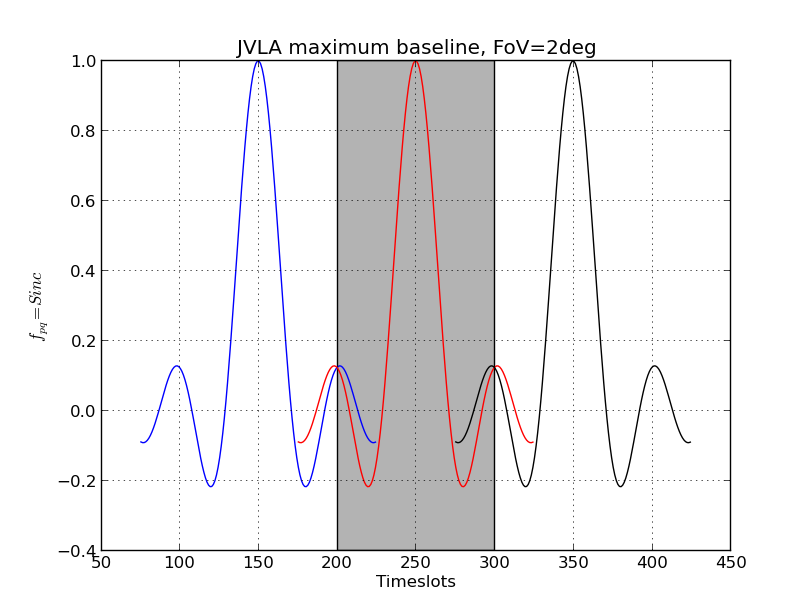
\includegraphics[width=1\textwidth]{./Figures/corrSigVLAMxBl_overlapLdelta.png}\caption{Overlap 
		\textit{BDWF's}: $\Delta_u t= [225, 250]$.}\label{fig:corrSigVLAMxBl_overlapLdelta}\end{minipage}
\begin{minipage}{0.38\linewidth}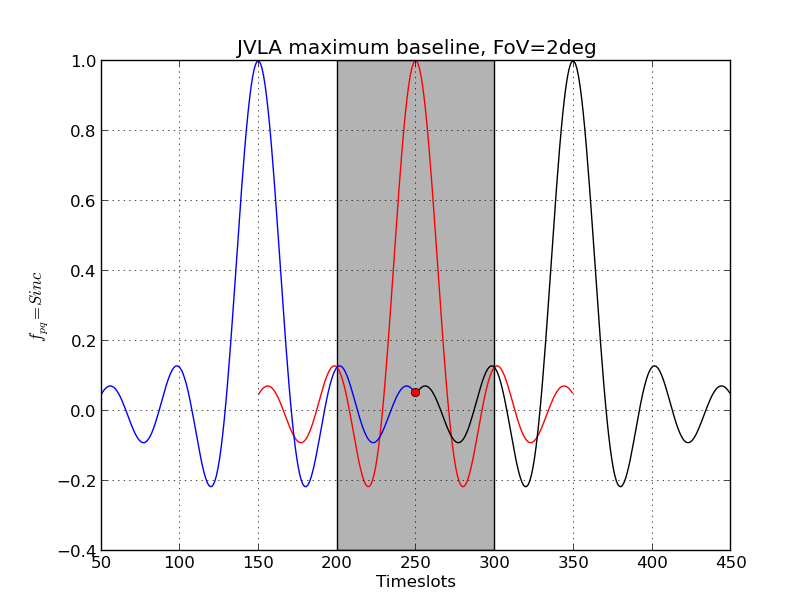
\includegraphics[width=1\textwidth]{./Figures/corrSigVLAMxBl.png}\caption{Overlap 
		\textit{BDWF's}: $\Delta_u t=\{250\}$.}\label{fig:corrSigVLAMxBl}\end{minipage}
  \hspace{1cm} 
\begin{minipage}{0.38\linewidth}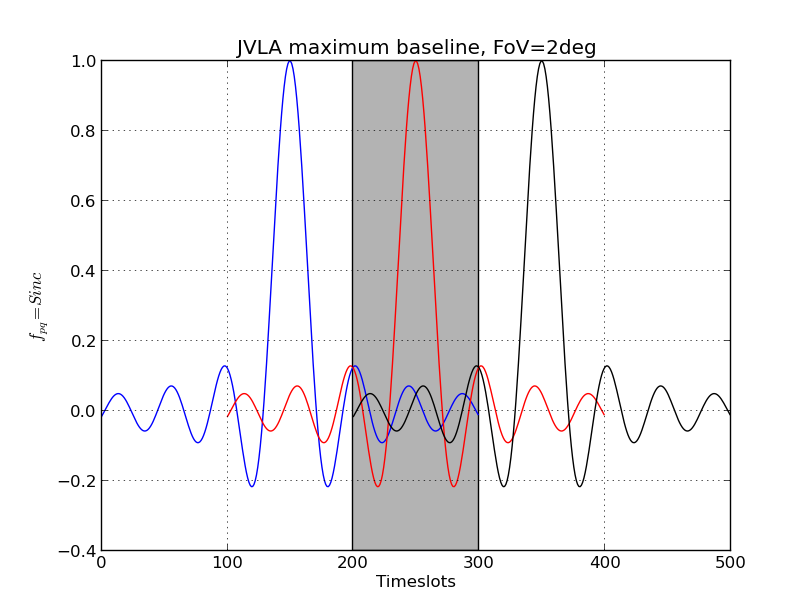
\includegraphics[width=1\textwidth]{./Figures/corrSigVLAMxBl_overlapGdelta.png}\caption{Overlap 
		\textit{BDWF's}: $\Delta_u t=\emptyset$.}\label{fig:corrSigVLAMxBl_overlapGdelta}\end{minipage}
\end{figure*}
\begin{figure*}
 \centering
    \begin{minipage}{0.38\linewidth}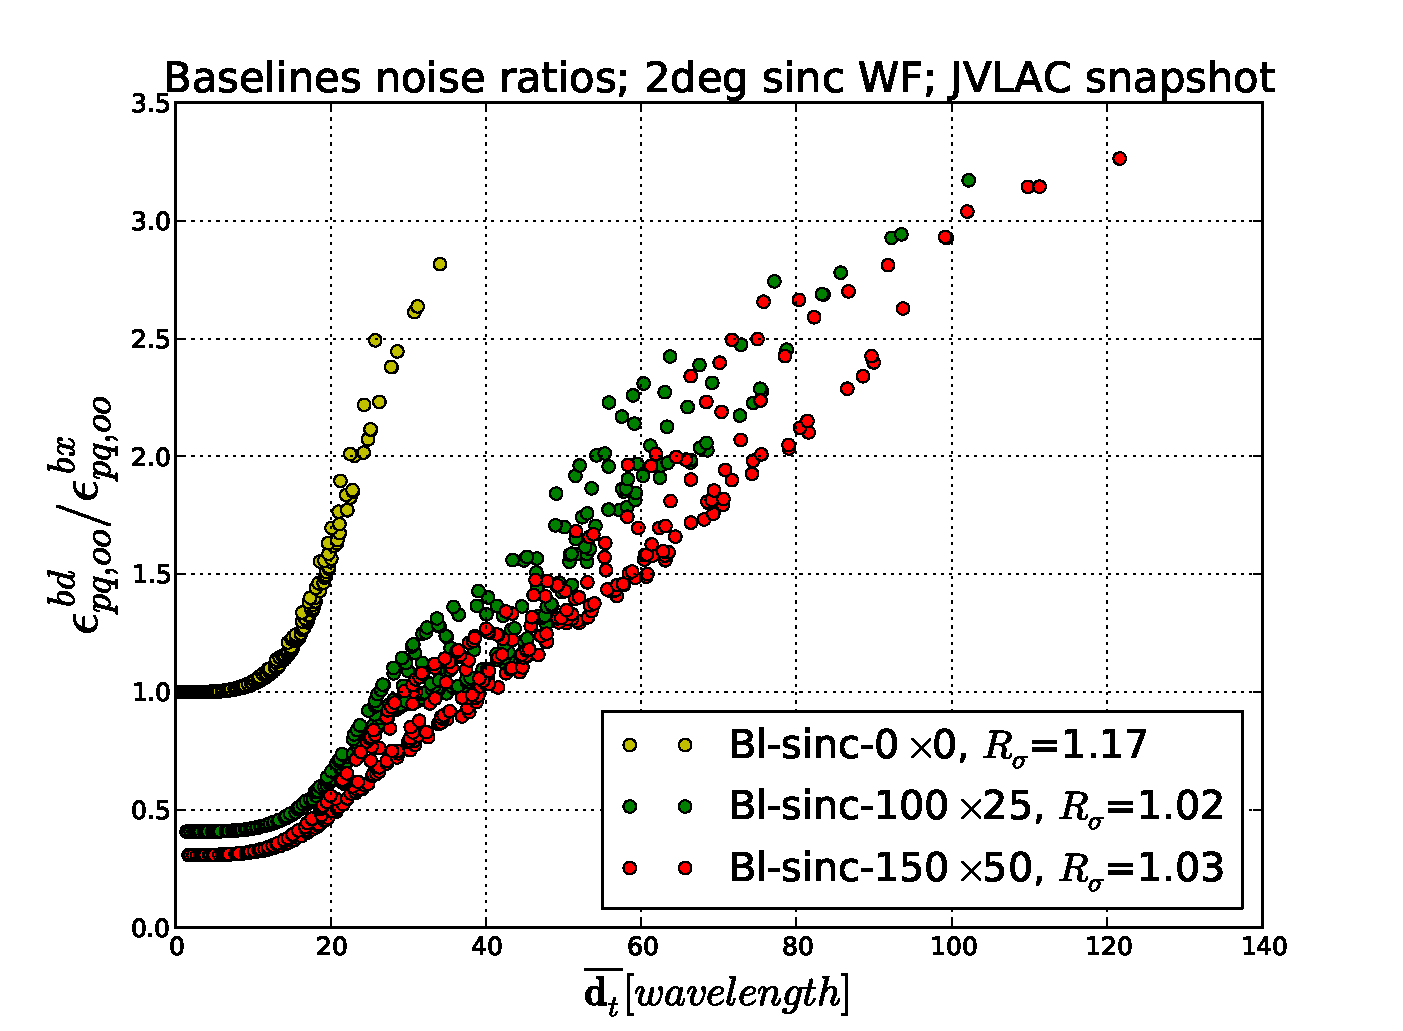
\includegraphics[width=1\textwidth]{./Figures/per-baseline-noise-ratio-sinc.pdf}
  \caption{Per baseline noise ratio of Bl-sinc-W$n_{lt}\times n_{l\nu}$ and averaging}\label{fig:per-baseline-noise-ratio-sinc}
  \end{minipage}
  \hspace{1cm}
  \begin{minipage}{0.38\linewidth}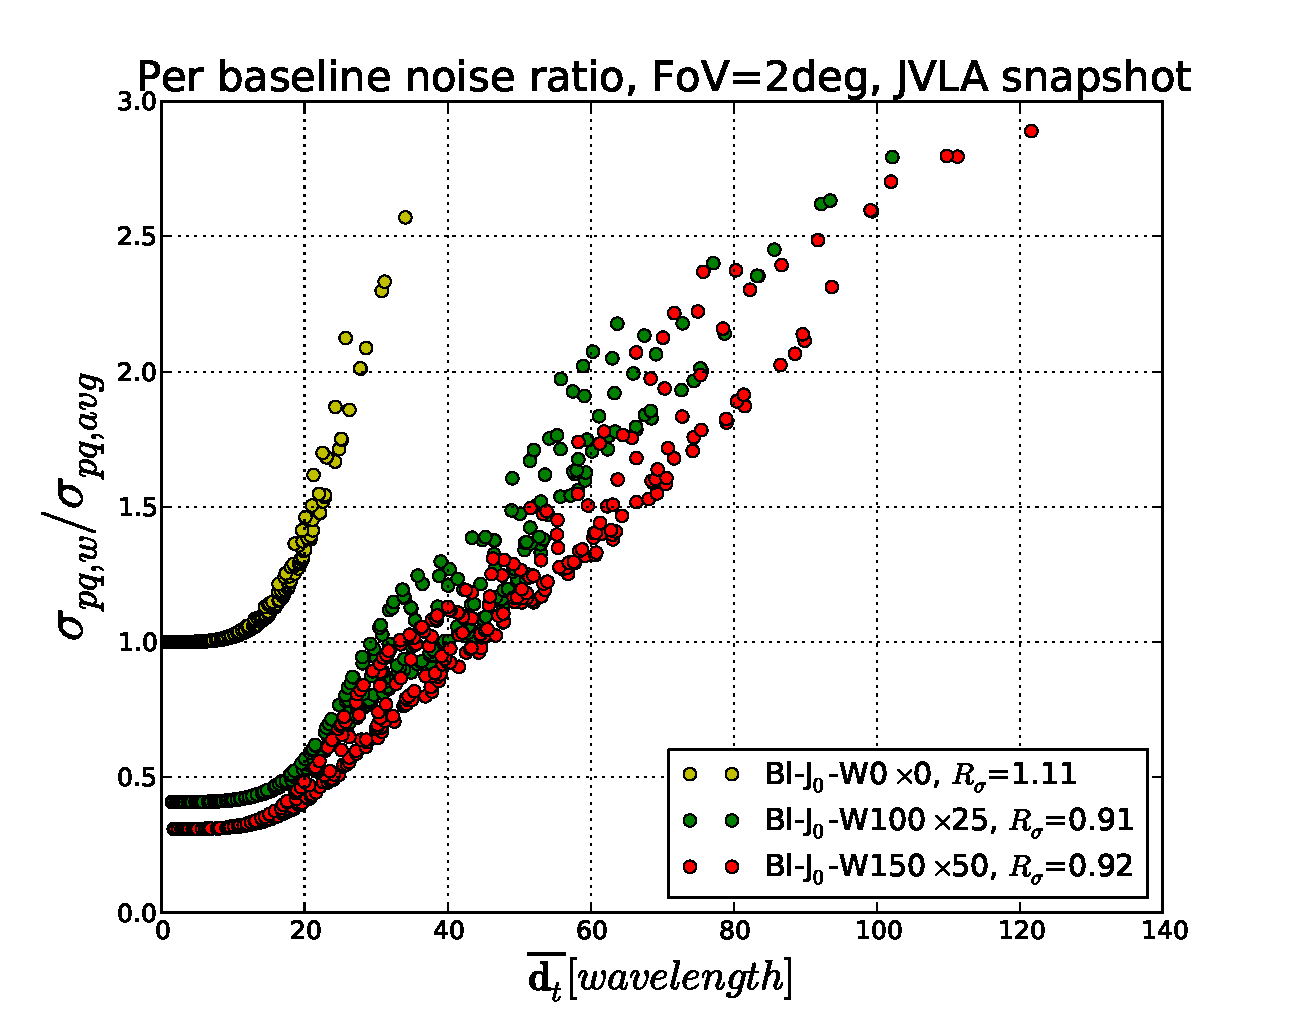
\includegraphics[width=1\textwidth]{./Figures/per-baseline-noise-ratio-bessel.pdf}
  \caption{Per baseline noise ratio of Bl-J$_0$-W$n_{lt}\times n_{l\nu}$ and 
averaging}\label{fig:per-baseline-noise-ratio-bessel}\end{minipage}
  \begin{minipage}{0.38\linewidth}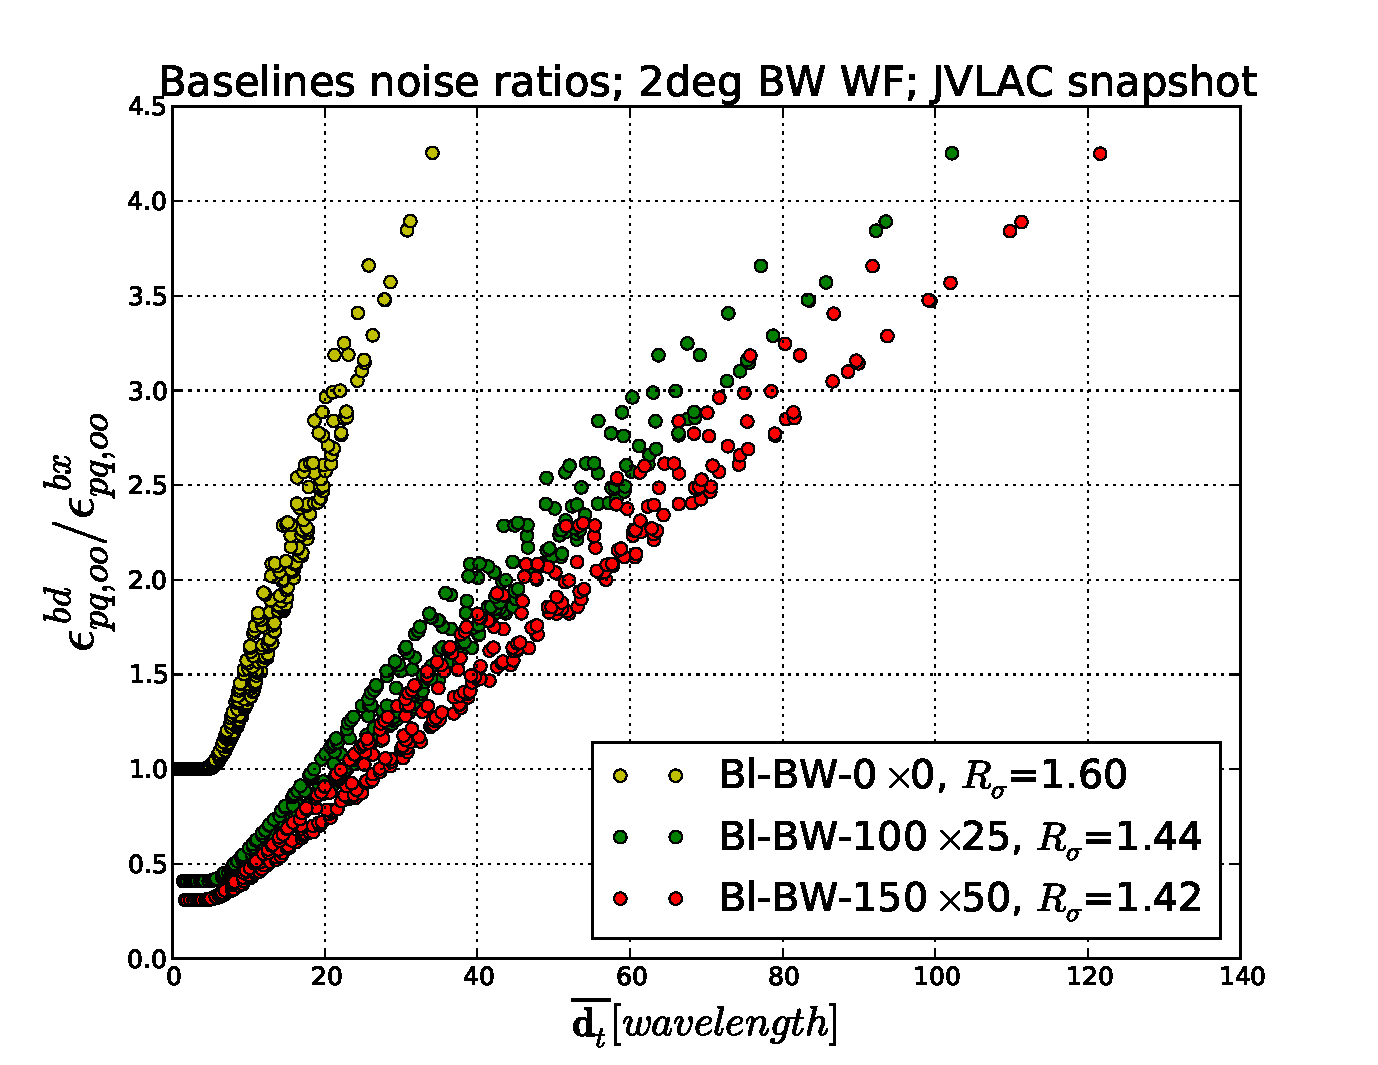
\includegraphics[width=1\textwidth]{./Figures/per-baseline-noise-ratio-BW.pdf}
  \caption{Per baseline noise ratio of Bl-BW-W$n_{lt}\times n_{l\nu}$ and averaging}\label{fig:per-baseline-noise-ratio-BW}
  \end{minipage}
\end{figure*}
\begin{itemize}
 \item In Fig.\ref{fig:per-baseline-noise-ratio-sinc}, Fig.\ref{fig:per-baseline-noise-ratio-bessel} 
and \ref{fig:per-baseline-noise-ratio-BW} we plotted the ratio of per baseline theoretical rms noise of the baseline dependent 
windowing function taken under consideration by the one of boxcar averaging. The ratio is plotted as a function of 
$\overline{\mathbf{d}}_t$ (the mean of  $(u,v)$ distance). These figures shows that, the noise increases with baseline length.
   \item On shorter baselines, the noise using the baseline dependent windowing function is approximately the same with the one of boxcar
averaging. However, the noise drops significantly with the number of  overlap time and frequency bins. As mention above, this is because on 
shorter  baselines, the baseline dependent windowing function are closer to the boxcar window, and when the number of overlap time  and 
frequency  bins increases, we have:
\begin{eqnarray*}
 \frac{\sigma_{pq, w}}{\sigma_{pq,avg}} &\approx& \Bigg(\frac{n_t n_{\nu}}{(n_t + n_{lt} + n_{rt})(n_{\nu} + n_{l\nu} + 
n_{r\nu})}\Bigg)^{\frac{1}{2}}
\end{eqnarray*}
\end{itemize}
The tables below summarized the interferometer theoretical rms noise ratio and the simulation one.\\
\begin{tabular}{*3{c}}
 \multicolumn{3}{|c|}{}\\
 \begin{tabular}{|l|l|l|l|}
  \footnotesize $f_{pq}$ &\textbf{\footnotesize Theoretical}&\textbf{\footnotesize Simulation}\\
  \hline\hline
  {\footnotesize Bl-sinc-W0$\times$0} &{\footnotesize $1.17$} &{\footnotesize $1.23$}\\
  {\footnotesize Bl-J$_0$-W0$\times$0} &{\footnotesize  $1.11$}&{\footnotesize  $1.14$}\\
  {\footnotesize Bl-BW-W0$\times$0} & {\footnotesize $1.16$}&{\footnotesize  $1.55$}\\
  \end{tabular}& \label{BDWBnoise}
\end{tabular}\\
\begin{tabular}{*3{c}}
 \multicolumn{3}{|c|}{}\\
 \begin{tabular}{|l|l|l|l|}
  \footnotesize $g_{pq}$ &\textbf{\footnotesize Theoretical}&\textbf{\footnotesize Simulation}\\
  \hline\hline
  {\footnotesize Bl-sinc-W100$\times$25} &{\footnotesize $1.02$} &{\footnotesize $1.18$}\\
  {\footnotesize Bl-J$_0$-W100$\times$25} &{\footnotesize  $0.91$}&{\footnotesize  $1.08$}\\
  {\footnotesize Bl-BW-W100$\times$25} & {\footnotesize $1.44$}&{\footnotesize  $1.49$}\\
  \hline
  {\footnotesize Bl-sinc-W150$\times$50} &{\footnotesize $1.03$} &{\footnotesize $1.27$}\\
  {\footnotesize Bl-J$_0$-W150$\times$50} &{\footnotesize  $0.92$}&{\footnotesize  $1.13$}\\
  {\footnotesize Bl-BW-W150$\times$50} & {\footnotesize $1.42$}&{\footnotesize  $1.44$}\\
  \end{tabular}& \label{BDWBnoise}
\end{tabular}
\section{Simulations and results}
In order to test the algorithms described in section \ref{baseline1} and section \ref{baseline2}, we performed  multiple tests on JVLA 
simulated measurement sets (MS). In 
this section we summarized and discussed those results. Two MS are used in 
our simulation, a high resolution MS (HR-MS) that contains the observed JVLA data of short integration time and frequency, a low 
resolution 
MS (LR-MS), where the results of boxcar averaging or baseline dependent windowing functions are saved. To apply the second algorithm 
described in section \ref{baseline2}, the following conditions have to be satisfied:
\begin{enumerate}
 \item If $t^{hrms}_{start}$ and $t^{lrms}_{start}$ are the starting time of the HR-MS and LR-MS respectively. $n_{t,ovlp}$ the number 
of timeslots extended across the time direction, and  $\Delta t^{hrms}$ the HR-MS integration time, then 
      %\begin{eqnarray*}
	    $t^{lrms}_{start}\geq t^{hrms}_{start} + n_{t,ovlp}\times \Delta t^{hrms}$. 
      %\end{eqnarray*}
  \item If $t^{hrms}_{end}$ and $t^{lrms}_{end}$ are the ending time of the HR-MS and LR-MS respectively, then 
      %\begin{eqnarray*}
	    $t^{lrms}_{end}\leq t^{hrms}_{end} + n_{t,ovlp}\times \Delta t^{hrms}$. 
      %\end{eqnarray*}
 \item If $\nu^{hrms}_{start}$ and $\nu^{lrms}_{start}$ are the starting frequency of the HR-MS and LR-MS respectively. $n_{\nu,ovlp}$ 
the number of channels extended across the frequency direction, and  $\Delta \nu^{hrms}$ the HR-MS width, then 
      %\begin{eqnarray*}
	    $\nu^{lrms}_{start} \geq \nu^{hrms}_{start} + n_{\nu,ovlp}\times \Delta \nu^{hrms}$. 
      %\end{eqnarray*}
 \item If $\nu^{hrms}_{end}$ and $\nu^{lrms}_{end}$ are the ending frequency of the HR-MS and LR-MS respectively, then 
      %\begin{eqnarray*}
	    $\nu^{lrms}_{end} \leq \nu^{hrms}_{end} + n_{\nu,ovlp}\times \Delta \nu^{hrms}$. 
      %\end{eqnarray*}
\end{enumerate}
\subsection{Smearing elimination and out FoV suppression}
We considered $40$ different sky models each  containing a 1Jy source; the sky models differ from each other by the source coordinates. 
The reason for having  only one source in the sky model is to avoid standard imaging artefacts in the sky maps, which 
can affect the brightness of sources. Another obvious problem is the  CLEAN algorithm \citep{cornwell1999deconvolution}, which does not 
created 
perfect clean maps. Therefore we need to avoid sideslobes confusion. Each of the sky model is simulated 
with a JVLA HR-MS of 7min30s snapshot synthesis, with a $\Delta t^{hrms}=1.5s$ integration 
time at 1.4GHz,  with 150 channels of width $\Delta \nu^{hrms}$=125kHz.  Each HR-MS is then processed with boxcar averaging and baseline 
dependent windowing function averaging the results are saved into a LR-MS of 1min30s synthesis, with a 150s integration time,  with 1 
channels of width 6.25MHz. We 
considered, $\{t^{hrms}_{start},\nu^{hrms}_{start}\}=\{0s,125kHz\}$, $\{t^{lrms}_{start},\nu^{lrms}_{start}\}=\{1min30s,6250kHz\}$, 
$\{t^{hrms}_{end},\nu^{hrms}_{end}\}=\{7min30s,18750kHz\}$, $\{t^{lrms}_{end},\nu^{lrms}_{end}\}=\{6min,12500kHzkHz\}$, 
$n_{t,ovlp}=\{0,100,150\}$ 
and $n_{\nu,ovlp}=\{0,25,50\}$.\\
In Fig.\ref{fig:Bl-sinc-FoV2}- Fig.\ref{fig:Bl-bessel-FoV4} we
%Fig.\ref{fig:Bl-sinc-FoV4}, Fig.\ref{fig:Bl-bessel-FoV2} and
show the recovered source brightness as a function of  distance from the phase centre for boxcar averaging and the baseline dependent 
windowing functions we are considering. We considered three cases of the sinc ($Bl$-$sinc$ $W n_{t,ovlp} \times n_{\nu,ovlp}$), the Bessel 
of the first kind of order zero ($Bl$-J$_0$ $W n_{t,ovlp} \times n_{\nu,ovlp}$) and the Butterwordth ($Bl$-$BW$ $W n_{t,ovlp} \times 
n_{\nu,ovlp}$),  with  $n_{t,ovlp}=\{0,100,150\}$ and $n_{\nu,ovlp}=\{0,25,50\}$). We evaluated the loss in signal 
amplitude with longer LR-MS integration time intervals $\Delta t^{lrms}=150s$ and wider LR-MS integration frequency intervals $\Delta 
\nu^{lrms}=6250kHz$. We furthermore evaluated the  noise ratio, $\mathcal{R}_{\sigma}=\frac{\sigma_{w}}{\sigma_{Avg}}$ (with $\sigma_{w}$  
the resulting noise of the filter under consideration and $\sigma_{Avg}$ the noise of simple averaging).\\
% $r$: source position in degrees.}
These results show that:
\begin{itemize}
 \item We recover more than $90\%$ of the source brightness within $\approx 75\%$ of the FoV using $Bl$-$sinc$-$W0 \times 0$, 
      $Bl$-J$_0$-$W0\times0$ and $Bl$-BW-$W0\times0$. However, boxcar averaging is better at suppressing out FoV sources. 
 \item We recover more than $90\%$ of the source brightness within $\approx 95\%$ of the FoV with the overlap sinc and J$_0$. As 
mention in section \ref{subsec:Windowing functions} the reason for this is that, the overlap filter is an accurate practical evaluation of 
the window theoretical representation\footnote{windowing function theoretically extend to infinitely}. This is not the case with the 
overlap Butterwordth because the Butterwordth is similar to the boxcar at the passband and produced less signal leakage at the 
transition band compare to the boxcar. 
 \item Also note that for the overlap filters, out FoV source suppression is significantly improved.  When
looking at these figures, it appears that the curves of the overlaps filters are below the one of boxcar averaging when the source is out 
FoV. These overlapping windowing functions performed much better than boxcar averaging up to  $\approx 99\%$ of out FoV source flux.
  \item  When
looking at these figures, it appears that the sinc window conserved the signal within the FoV compared to J$_0$, while J$_0$ suppressed the 
signal out of the FoV compared to the sinc. However, the reason for 
this is that
the main lobe width of the sinc is narrower than that of J$_0$ and J$_0$ has low 
sidelobes level compared to the sinc.
\end{itemize}
When performing the baseline dependent filters, smearing was eliminated within the FoV while we compressed 
the data by integrating over a large time interval and wider frequency interval of a LR-MS. However,
the overlap baseline dependent filters significantly suppressed the source  when the source is out of the FoV  to a greater extent than 
boxcar averaging. Thus,
in all cases the SNR obtained using these methods is greater than obtained using boxcar averaging even as there is loss in 
sensitivity.
\subsection{Maximal integration}
In this section, we evaluated the maximum frequency and time integration intervals  that can be 
considered in the frequency and the time 
directions without smearing in the FoV, with optimal source suppression out of the FoV. We considered $6$ different sky 
models each  containing a 1Jy source; the sky models differ from each other by the source distance, $r$ from the phase centre
($r=\{0.09^\circ,0.25^\circ,0.5^\circ,1^\circ,1.5^\circ, 2^\circ\}$).
\subsubsection{Frequency direction}
The baseline dependent windowing functions under considerations and the boxcar averaging are performed in the frequency direction.
The sky models is simulated with a JVLA HR-MS of 1 timeslot of width $\Delta t^{hrms}=0.1s$ at $1.4$GHz. The raison of a short HR-MS 
integration time is to avoid time direction smearing. We considered 150 channels, and varied the width, $\Delta \nu^{hrms}$ in the interval 
$[125,1187.5]$kHz. The result of the process was saved into a LR-MS of 1 timeslot of width $\Delta t^{lrms}=0.1s$ at $1.4$GHz, with 1 
channel of width $\Delta \nu^{hrms}\times50$kHz. We considered, $\nu^{hrms}_{start}=\Delta \nu^{hrms}kHz$, 
$\nu^{lrms}_{start}=\nu^{hrms}_{start}\times50 kHz$, $\nu^{hrms}_{end}=\nu^{hrms}_{start}\times150 kHz$ and 
$\nu^{lrms}_{end}=\nu^{hrms}_{start}\times100 kHz$.\\
In Fig.\ref{fig:max-integ-freq-sinc-w1x1-fov2}-Fig.\ref{fig:max-integ-freq-butter-w1x50-fov2} we compared the result of boxcar frequency 
averaging and of  Bl-sinc-$W n_{\nu,ovlp}$, Bl-J$_0$ $W n_{\nu,ovlp}$, Bl-BW-$W n_{\nu,ovlp}$ performed in the frequency 
direction. We took $n_{\nu,ovlp}=\{0,50\}$ the number of frequency overlap bins. These results show that:
\begin{itemize}
 \item Firstly,  we can integrate over a wider LR-MS frequency interval without a loss of signal 
amplitude. However, looking at these figures, the curves of the source at $0.09^{\circ},0.25^{\circ},0.5^{\circ}$ from the phase centre are 
closer to the affine equation $y=1$, which differ from the curves when the source is at $1^{\circ},1.5^{\circ}, 2^{\circ}$ from the phase 
centre.  
 \item Secondly, looking on Fig.\ref{fig:max-integ-freq-sinc-w1x50-fov2} and Fig.\ref{fig:max-integ-freq-bessel-w1x50-fov2}, when the source 
is at $1.5^{\circ}$ and $2^{\circ}$, the attenuation is significant within 
$[6.2,12.6]MHz$ with the overlap frequency direction filters compared to boxcar frequency averaging. This is not the case with Fig.
\ref{fig:max-integ-freq-butter-w1x50-fov2}. Nevertheless, out FoV source suppression start with the Butterwordth when the source is at 
$2.5^{\circ}$ or above (see Fig.\ref{fig:Bl-butter-FoV2}) 
 \item Finally, the sinc filter performed well on signal recovery compared to J$_0$ and J$_0$ suppressed 
the source when this is out of the FoV compared to the sinc.  
\end{itemize}
\subsubsection{Time direction}
In this case, each of these sky model is simulated with a JVLA HR-MS of $300$ timeslots synthesis, and we varied the integration time 
$\Delta t^{hrms}$ in the interval $[0.5,5.5]$s at 1.4GHz. We considered 1 channel of width, $\Delta \nu^{hrms}=125kHz$.   We 
therefore applied the actual method (simple averaging) and our methods both in the time direction then the result of each simulation was 
saved into a LR-MS of $100\times\Delta t^{hrms}s$ synthesis, with a $100\times\Delta t^{hrms}s$ integration time, with 1 channels of width 
$125kHz$. We considered, $t^{hrms}_{start}=0s$, $t^{lrms}_{start}=100$timeslots$\times\Delta t^{hrms} s$, 
$t^{hrms}_{end}=300$timeslots$\times\Delta t^{hrms}s$ and $t^{lrms}_{end}=200$timeslots$\times\Delta t^{hrms}s$.\\
We compared in Fig.\ref{fig:max-integ-time-sinc-w1x1-fov2} and Fig.\ref{fig:max-integ-time-sinc-w100x1-fov2}  the results of simple 
time averaging and the one of  $Bl$-$sinc$ $W n_{t,ovlp}$ performed in the time direction. We compared in 
Fig.\ref{fig:max-integ-time-bessel-w1x1-fov2} and Fig.\ref{fig:max-integ-time-bessel-w100x1-fov2} the results of simple time averaging 
and the one of  $Bl$-J$_0$ $W n_{t,ovlp}$. Here, we took $n_{t,ovlp}=\{0,100\}$ time overlap bins. These results 
showed that:
\begin{itemize}
 \item Firstly, we can significantly integrate over a longer LR-MS time interval without a lost of signal 
amplitude. However, looking at these figures, the curves of the source at $0.09^{\circ},0.25^{\circ},0.5^{\circ}$ from the phase centre are 
closer to the affine equation $y=1$, which differ from the curves when the source is at $1^{\circ},1.5^{\circ}, 2^{\circ}$ from the phase 
centre.  
 \item Secondly, looking on Fig.\ref{fig:max-integ-freq-sinc-w1x50-fov2} and 
\ref{fig:max-integ-freq-bessel-w1x50-fov2}, when the source is at $1.5^{\circ}$ and $2^{\circ}$, the attenuation is significant within 
$[50,150]$ with the overlap time direction filters compared to simple time averaging.
 \item Finally, the sinc filter performed well on signal recovery compare to the Bessel first kind and the Bessel first kind suppressed the 
source when this is out of the FoV compared to the sinc.  
\end{itemize}
\vspace{-0.5cm}
\subsubsection{Time and frequency direction}
In this case, each sky model is simulated with a JVLA HR-MS of $300$ timeslots synthesis, and varied  the integration time $\Delta 
t^{hrms}$ in $[0.5,5.5]s$ at $1.4GHz$.  We considered $150$ channels and varied the width $\Delta \nu^{hrms}$  within the interval $[ 
125.,750.]kHz$. We therefore applied the actual method (simple averaging) and our methods both in the frequency direction and time 
direction, each result was saved into a LR-MS of  $100$timeslots$\times\Delta t^{hrms}s$ synthesis, with $100$timeslots$\times\Delta 
t^{hrms}$ integration time and 1 channels of width $50$channels$\times\Delta \nu^{hrms}kHz$. We considered, $t^{hrms}_{start}=0s$, 
$t^{lrms}_{start}=100$timeslots$\times\Delta t^{hrms} s$, $t^{hrms}_{end}=300$timeslots$\times\Delta t^{hrms}s$ and 
$t^{lrms}_{end}=200$timeslots$\times\Delta t^{hrms}s$, $\nu^{hrms}_{start}=\Delta \nu^{hrms}kHz$, 
$\nu^{lrms}_{start}=\nu^{hrms}_{start}\times50 kHz$, $\nu^{hrms}_{end}=\nu^{hrms}_{start}\times150 kHz$ and 
$\nu^{lrms}_{end}=\nu^{hrms}_{start}\times100 kHz$.\\ 
We compared in Fig.\ref{fig:max-integ-timefreq-sinc-w1x1-fov2} and Fig.\ref{fig:max-integ-timefreq-sinc-w100x50-fov2}  the results of 
simple time and frequency averaging and the one of  $Bl$-$sinc$ $W n_{t,ovlp}\times n_{\nu,ovlp}$ performed in the time and frequency 
direction. We compared in Fig.\ref{fig:max-integ-timefreq-bessel-w1x1-fov2} and Fig.\ref{fig:max-integ-timefreq-bessel-w100x50-fov2} the 
results of simple time and frequency averaging and the one of  $Bl$-J$_0$ $W n_{t,ovlp}\times n_{\nu,ovlp}$ performed in the time and 
frequency direction. Here, we took $n_{t,ovlp}=\{0,100\}$ time overlap bins and $n_{\nu,ovlp}=\{0,50\}$ frequency overlap bins. These 
results showed that:
\begin{itemize}
 \item Firstly, we can significantly integrate over a longer LR-MS time interval and frequency interval at the same time without a lost of 
signal amplitude. However, looking at these figures, the curves of the source at $0.09^{\circ},0.25^{\circ},0.5^{\circ}$ from the phase 
centre are closer to the affine equation $y=1$, which differs from the curves when the source is at $1^{\circ},1.5^{\circ}, 2^{\circ}$ from 
the phase centre. 
 \item Secondly, looking on Fig.\ref{fig:max-integ-timefreq-sinc-w100x50-fov2} and \ref{fig:max-integ-timefreq-bessel-w100x50-fov2}, when 
the source is at $1.5^{\circ}$ and $2^{\circ}$, it appears that the curves of the overlaps filters are below the one of simple averaging. 
These suggest that, when we are integrating both over a wider LR-MS time interval and frequency interval, the source is suppressed 
significantly out of the FoV without any constraint on the integration time and frequency.
 \item Finally, the sinc filter performed well on signal recovery compared to the Bessel first kind and the Bessel first kind suppressed 
the 
source when this is out of the FoV compared to the sinc.  
\end{itemize}
\subsection{One strong source in the sky model and attenuation efficiency}
\begin{figure*}
  \centering
\begin{minipage}{0.36\linewidth}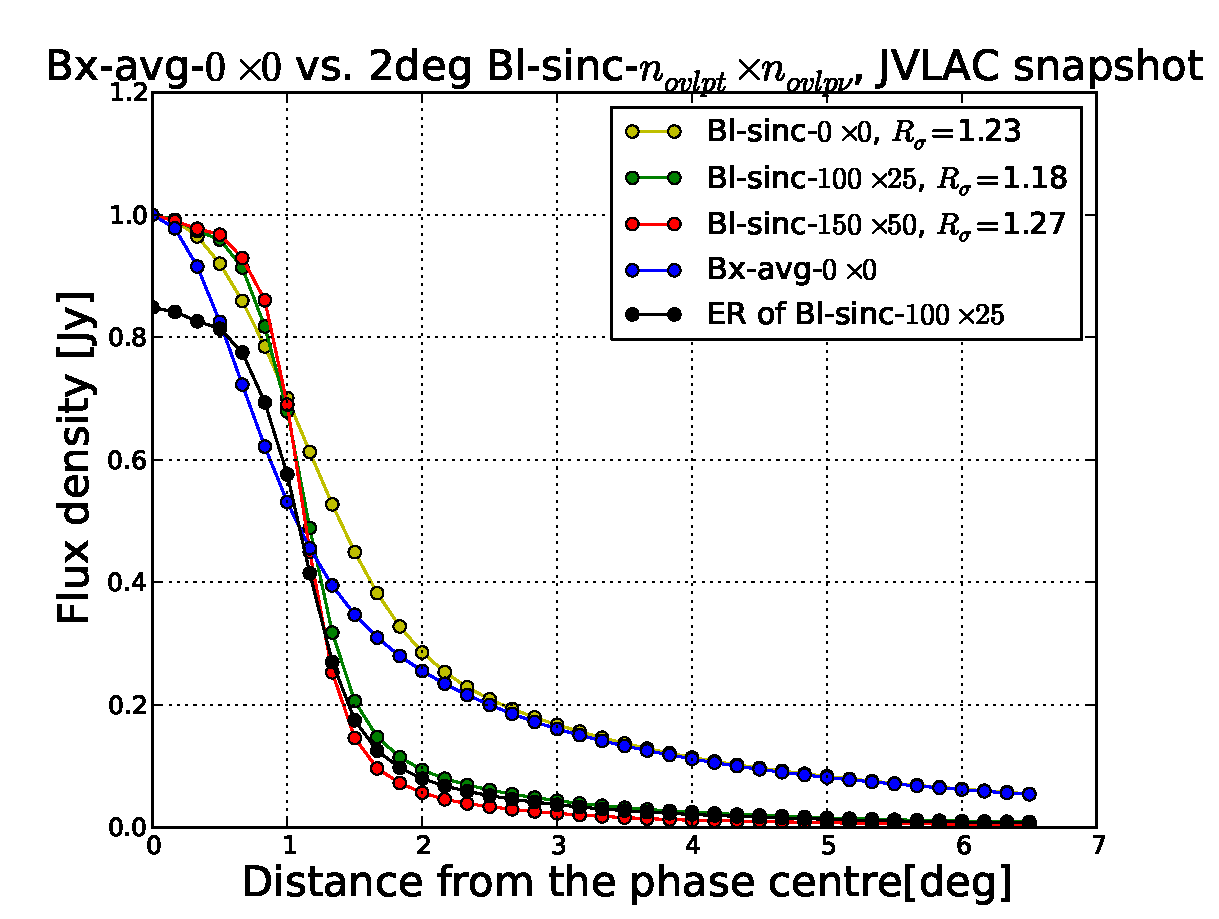
\includegraphics[width=1\textwidth]{./Figures/Bl-sinc-FoV2-vla.pdf}\caption{Time and frequency 
direction sinc filter applied on a $2^{\circ}$ FoV JVLA surveys observing a 1Jy source move from the phase centre for 150s integration 
synthesis at 6.25MHz bandwidth, natural weighting.}\label{fig:Bl-sinc-FoV2}\end{minipage}
\hspace{1cm}
\begin{minipage}{0.36\linewidth}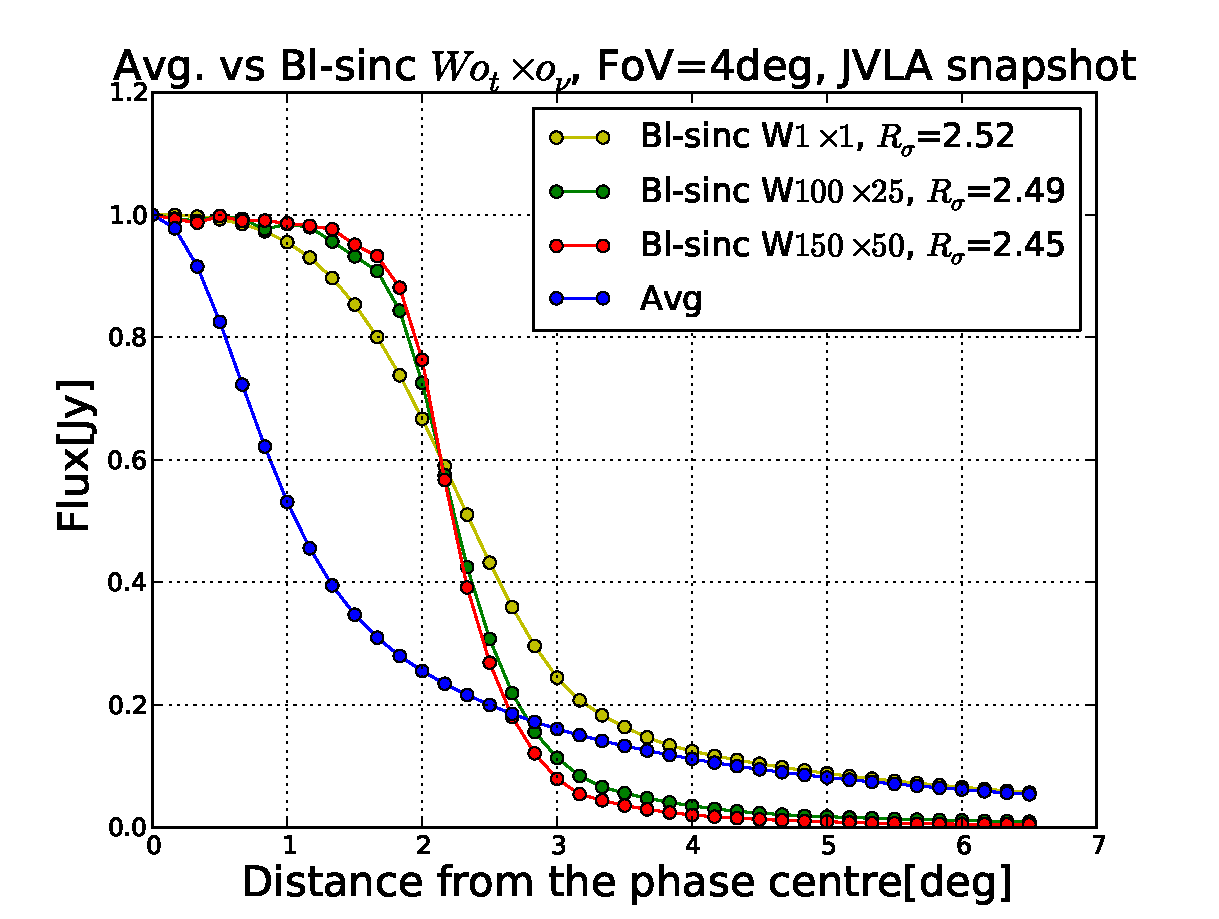
\includegraphics[width=1\textwidth]{./Figures/Bl-sinc-FoV4-vla.pdf}\caption{Time and frequency 
direction sinc filter applied on a $4^{\circ}$ FoV JVLA surveys observing a 1Jy source move from the phase centre for 150s integration 
synthesis at 6.25MHz bandwidth, natural weighting.}\label{fig:Bl-sinc-FoV4} 
\end{minipage}\\
\begin{minipage}{0.36\linewidth}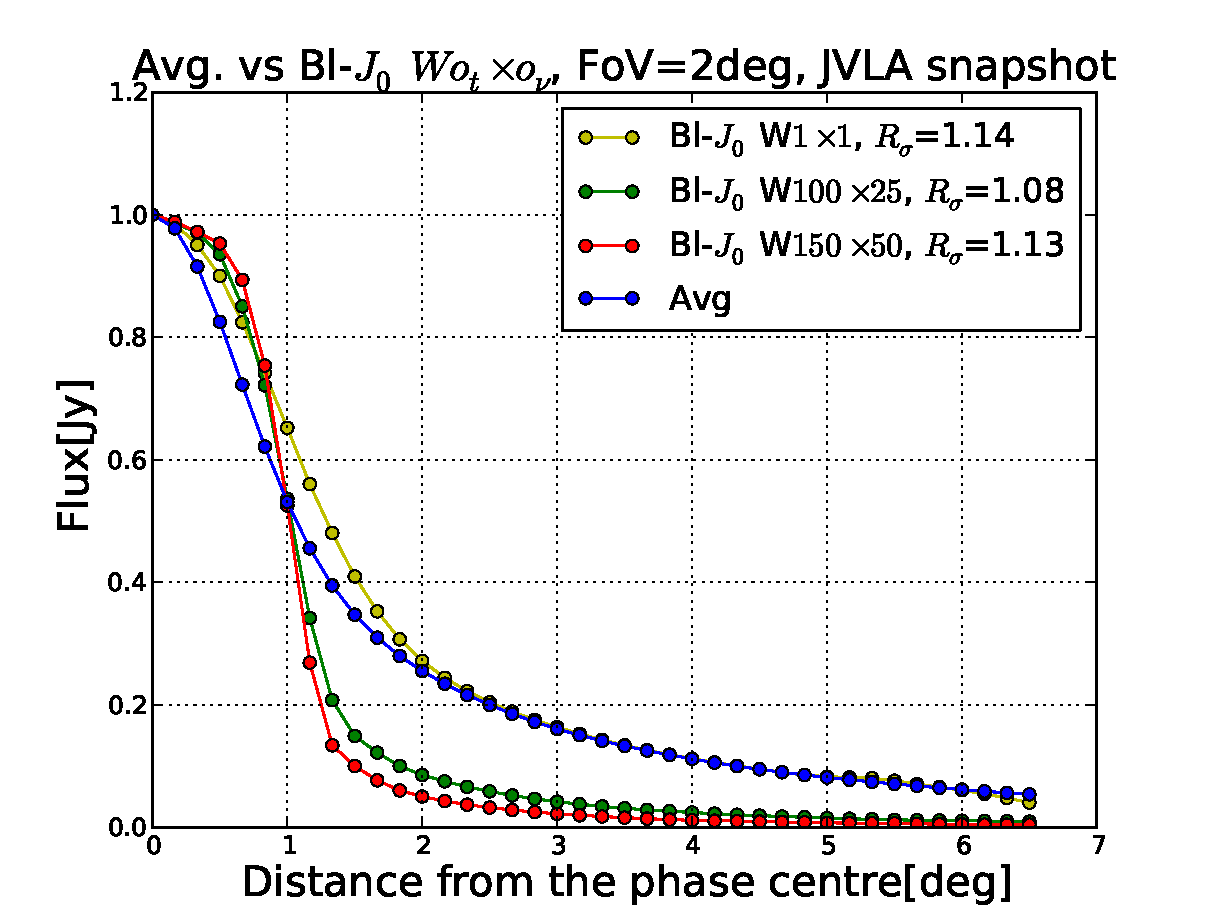
\includegraphics[width=1\textwidth]{./Figures/Bl-bessel-FoV2-vla.pdf}\caption{Time and frequency 
direction Bessel first kind filter applied on a $2^{\circ}$ FoV JVLA surveys observing a 1Jy source move from the phase centre for 150s 
integration synthesis at 6.25MHz bandwidth, natural weighting.}\label{fig:Bl-bessel-FoV2}\end{minipage}
\hspace{1cm}
\begin{minipage}{0.36\linewidth}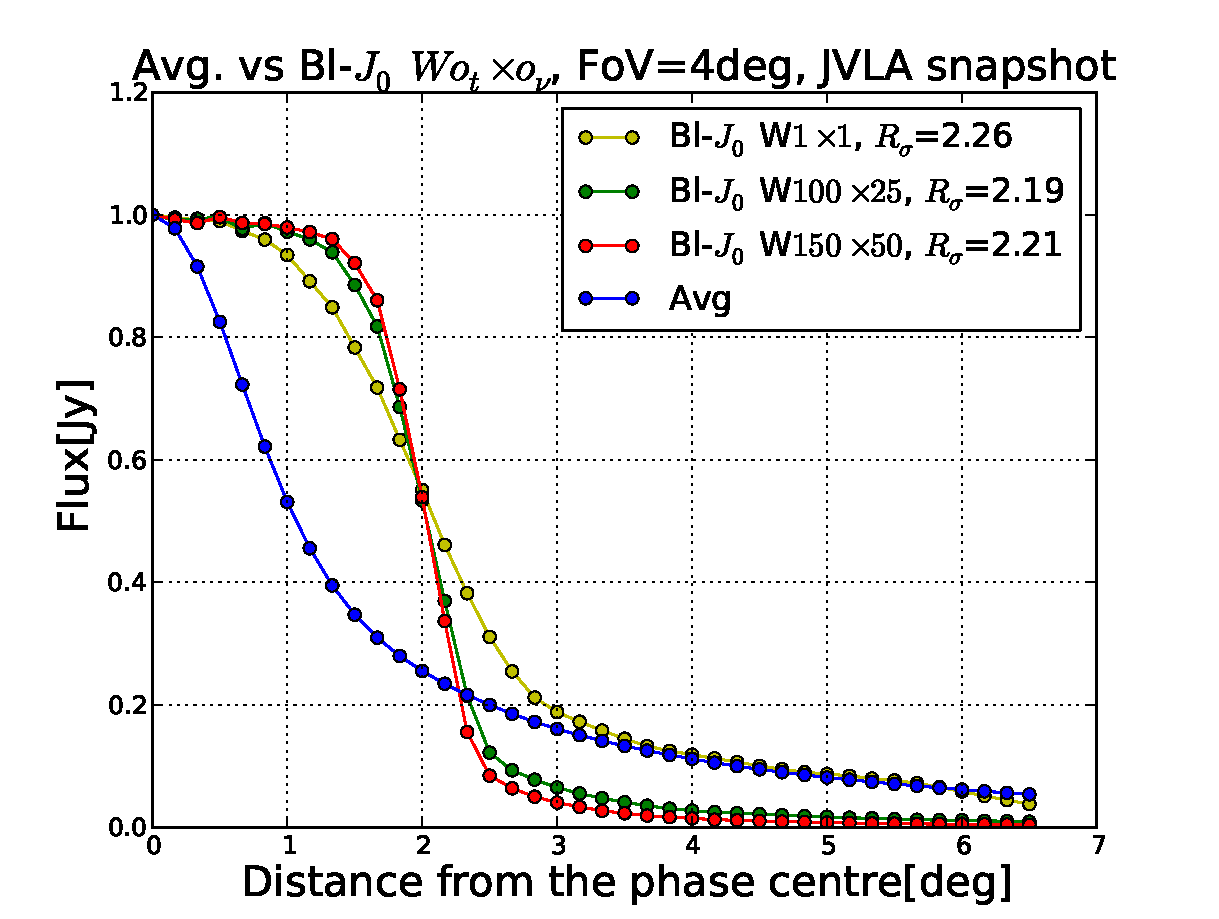
\includegraphics[width=1\textwidth]{./Figures/Bl-bessel-FoV4-vla.pdf}\caption{Time and frequency 
direction Bessel first kind filter applied on a $4^{\circ}$ FoV JVLA surveys observing a 1Jy source move from the phase centre for 150s 
integration synthesis at 6.25MHz bandwidth, natural weighting.}\label{fig:Bl-bessel-FoV4}\end{minipage}\\
\begin{minipage}{0.36\linewidth}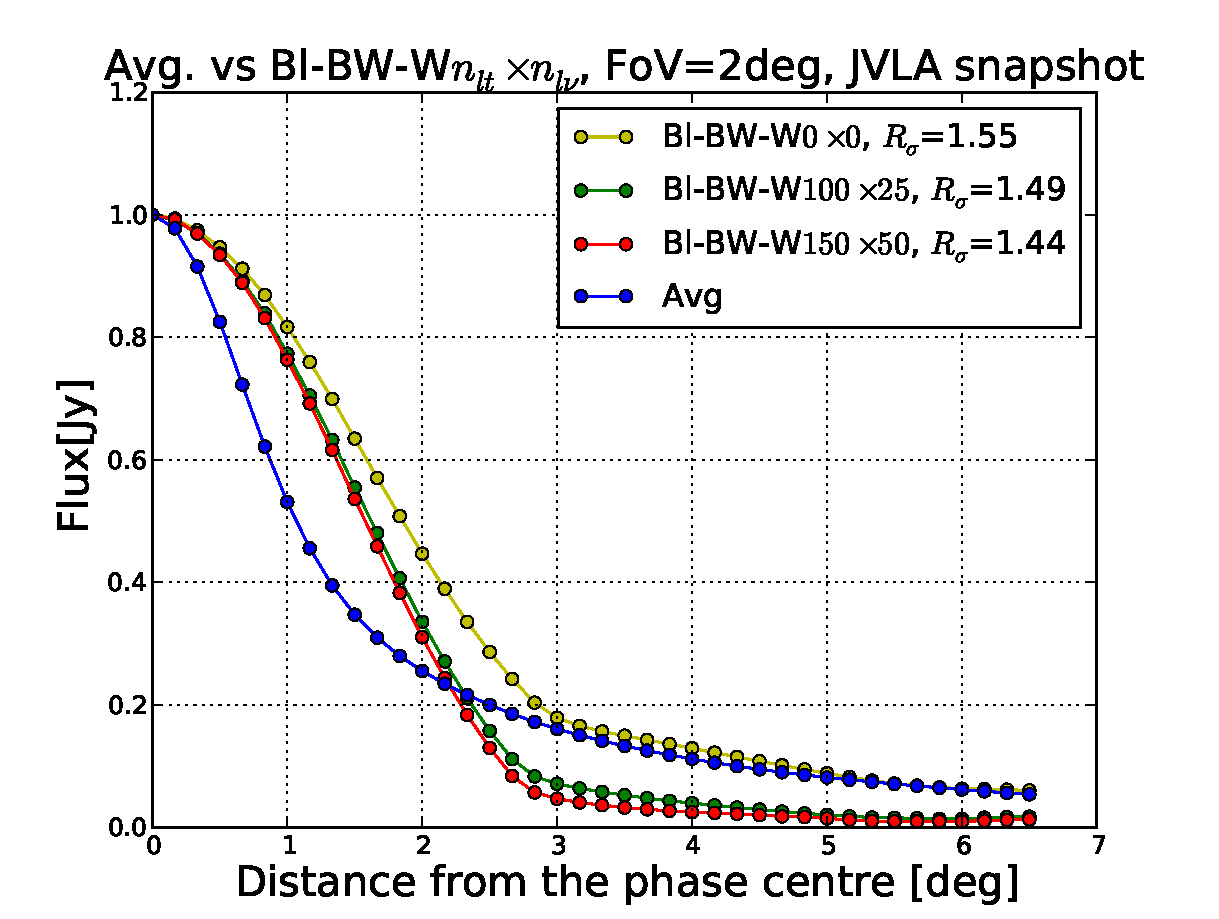
\includegraphics[width=1\textwidth]{./Figures/Bl-butter-FoV2-vla.pdf}\caption{Time and frequency 
direction Butterwordth filter applied on a $2^{\circ}$ FoV JVLA surveys observing a 1Jy source move from the phase centre for 
150s integration synthesis at 6.25MHz bandwidth, natural weighting.}\label{fig:Bl-butter-FoV2}\end{minipage}
\hspace{1cm}
\begin{minipage}{0.36\linewidth}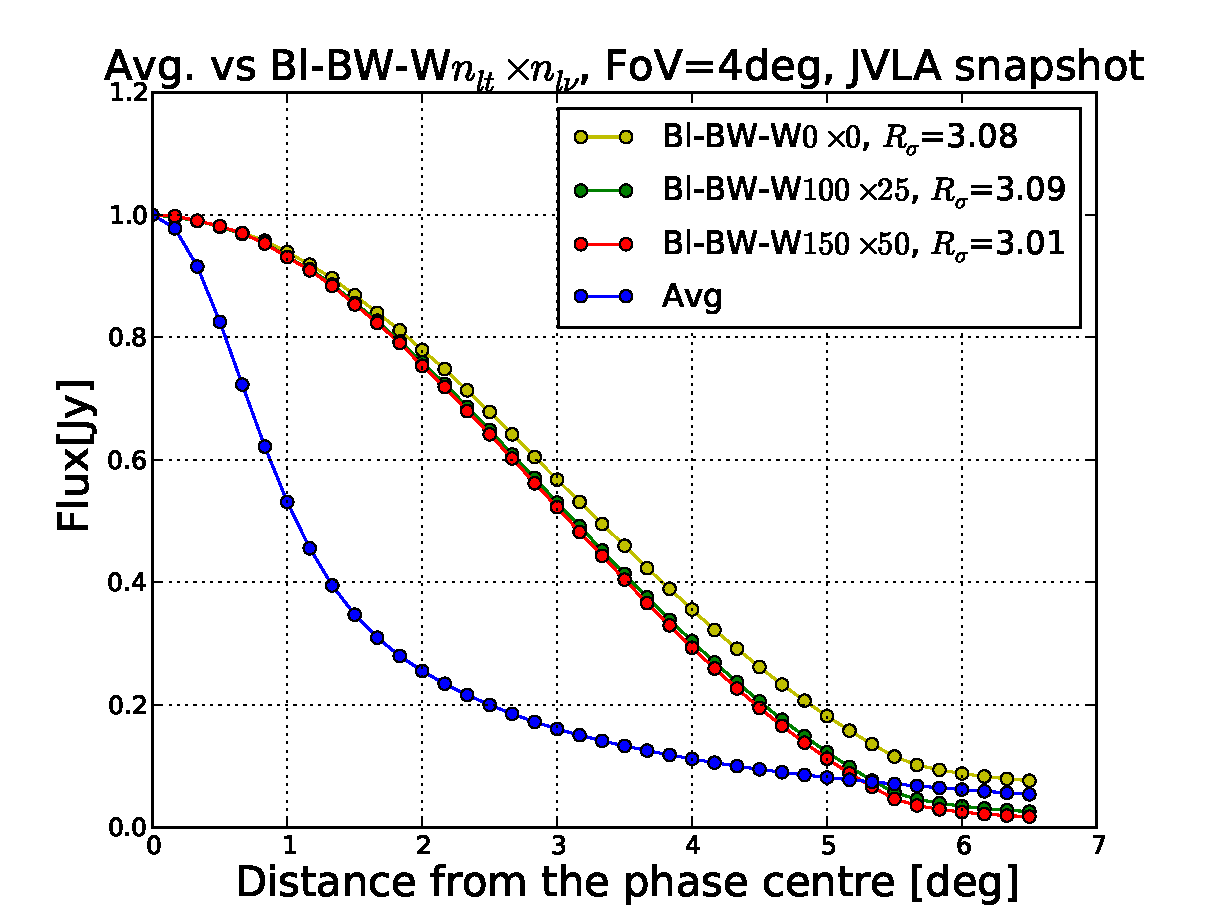
\includegraphics[width=1\textwidth]{./Figures/Bl-butter-FoV4-vla.pdf}\caption{Time and frequency 
direction Butterwordth filter applied on a $4^{\circ}$ FoV JVLA surveys observing a 1Jy source move from the phase centre for 150s 
integration synthesis at 6.25MHz bandwidth, natural weighting.}\label{fig:Bl-butter-FoV4}\end{minipage}
\end{figure*}
\begin{figure*}
  \centering
\begin{minipage}{0.36\linewidth}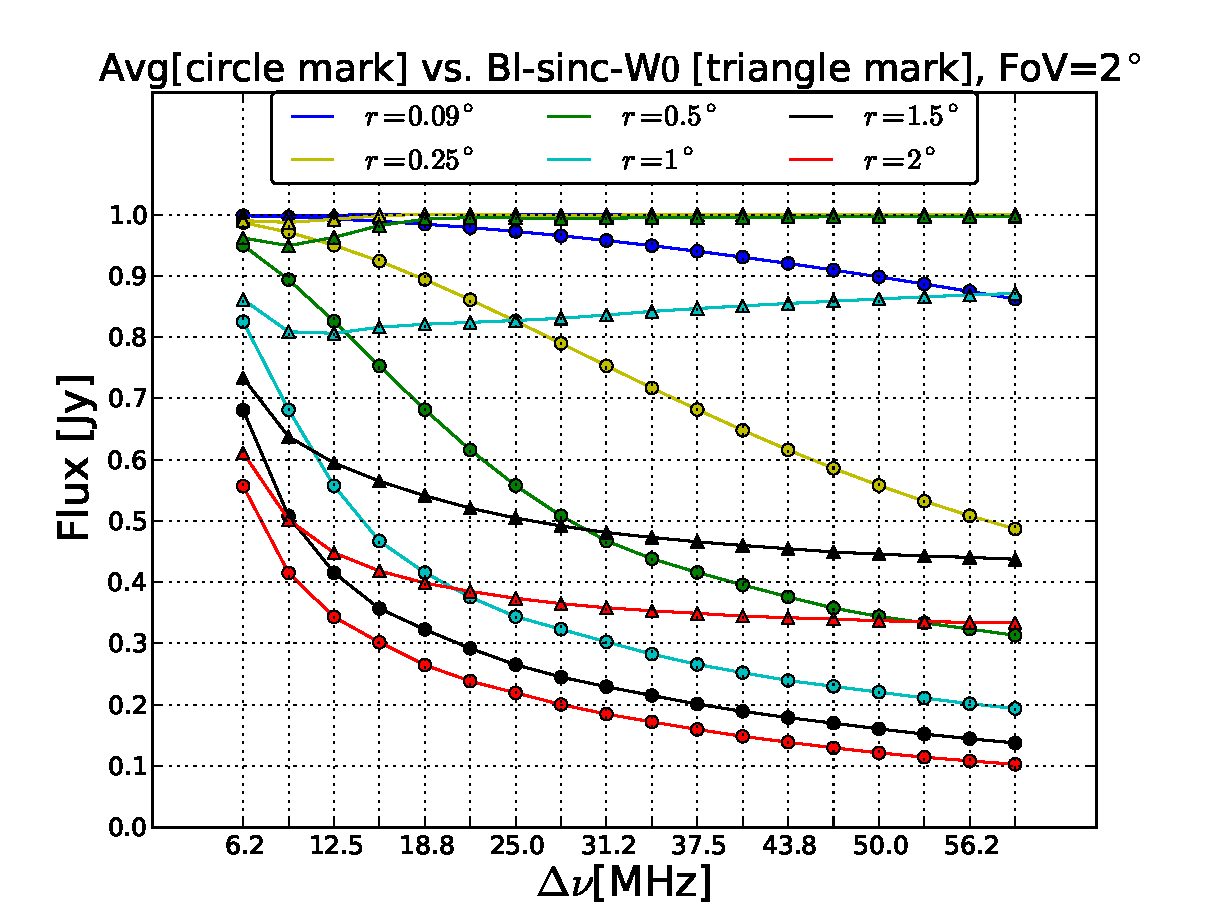
\includegraphics[width=1\textwidth]{./Figures/max-integ-freq-sinc-w1x1-fov2.pdf}
  \caption{Response to a 1Jy source at different positions, as a function of  bandwidth with $2^{\circ}$ frequency sinc filter.}
  \label{fig:max-integ-freq-sinc-w1x1-fov2}
\end{minipage}
\hspace{1cm}
\begin{minipage}{0.36\linewidth}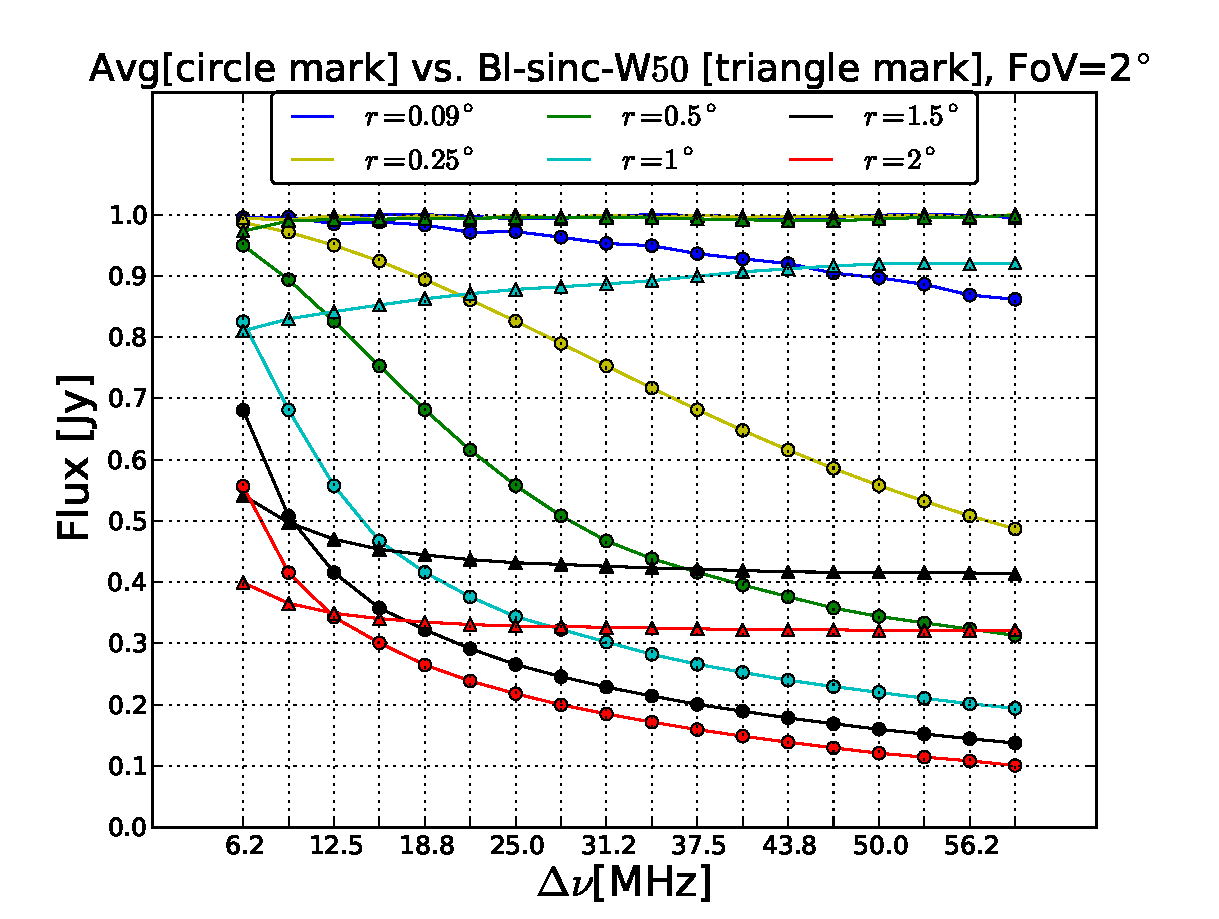
\includegraphics[width=1\textwidth]{./Figures/max-integ-freq-sinc-w1x50-fov2.pdf}
      \caption{Response to a 1Jy source at different positions, as a function of bandwidth with $2^{\circ}$ frequency overlap sinc filter.}
      \label{fig:max-integ-freq-sinc-w1x50-fov2}
      \end{minipage}\\
\begin{minipage}{0.36\linewidth}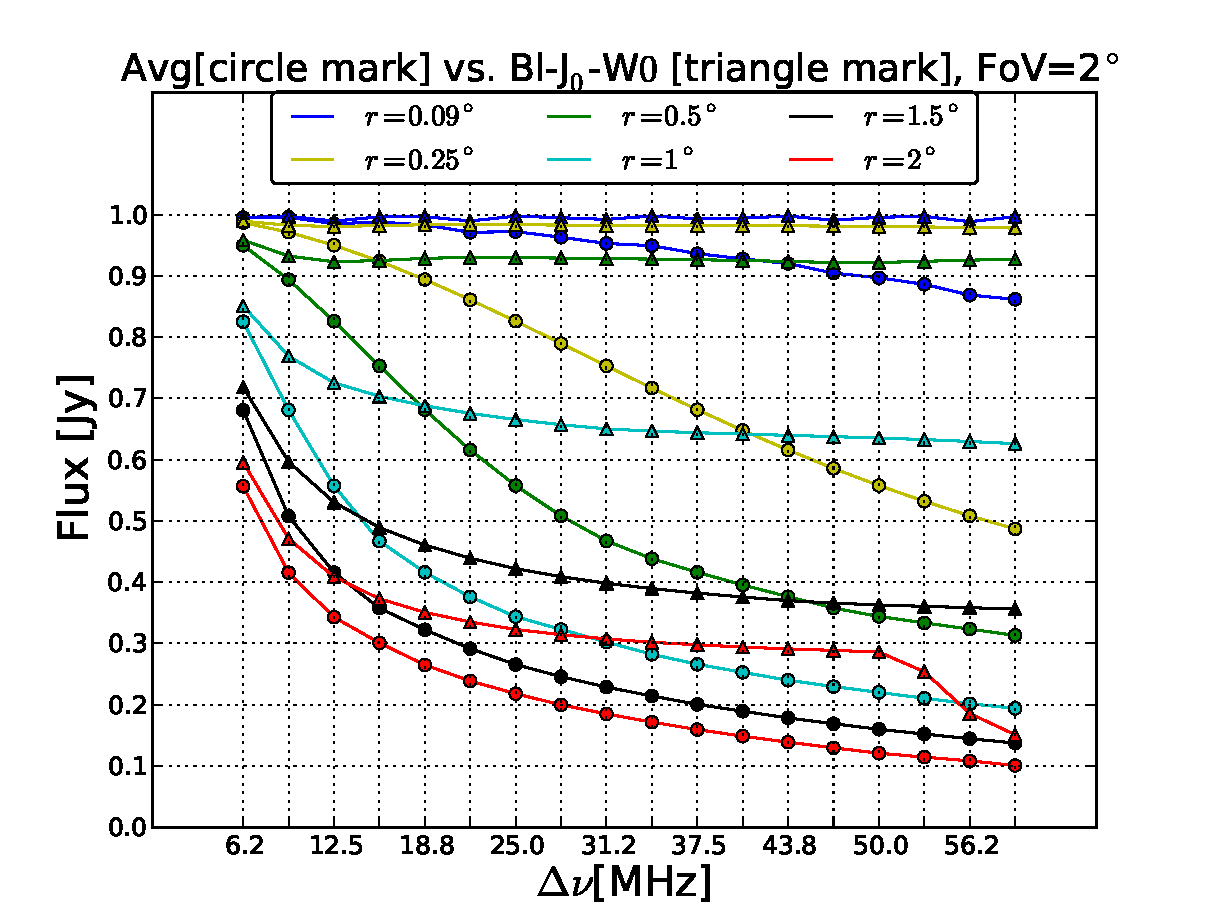
\includegraphics[width=1\textwidth]{./Figures/max-integ-freq-bessel-w1x1-fov2.pdf}
      \caption{Response to a 1Jy source at different positions, as a function of bandwidth with $2^{\circ}$ frequency Bessel first kind of 
order zero filter.}
      \label{fig:max-integ-freq-bessel-w1x1-fov2}
      \end{minipage}
\hspace{1cm}
\begin{minipage}{0.36\linewidth}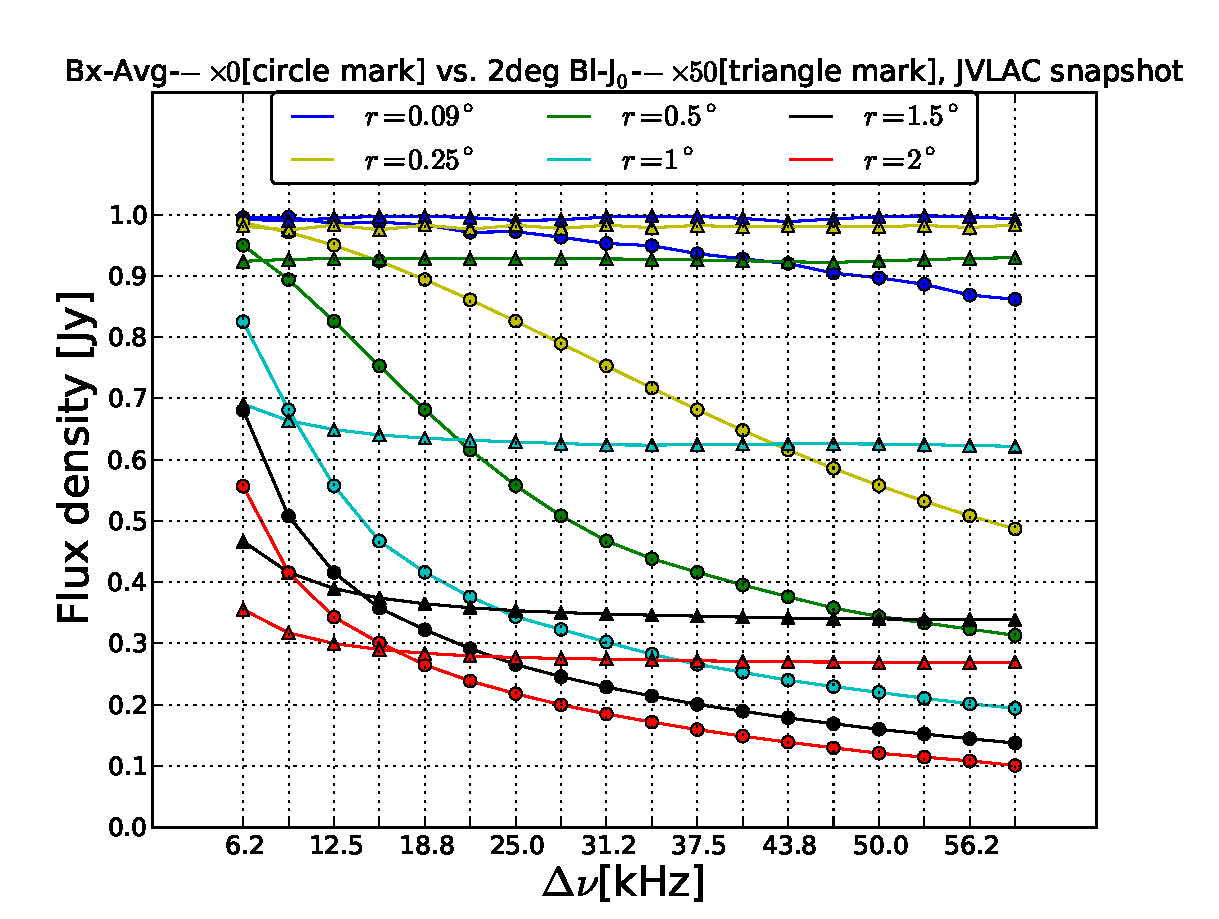
\includegraphics[width=1\textwidth]{./Figures/max-integ-freq-bessel-w1x50-fov2.pdf}
      \caption{Response to a 1Jy source at different positions, as a function of bandwidth with $2^{\circ}$ frequency overlap Bessel first 
kind filter of order zero filter.}
      \label{fig:max-integ-freq-bessel-w1x50-fov2}
      \end{minipage}
\begin{minipage}{0.36\linewidth}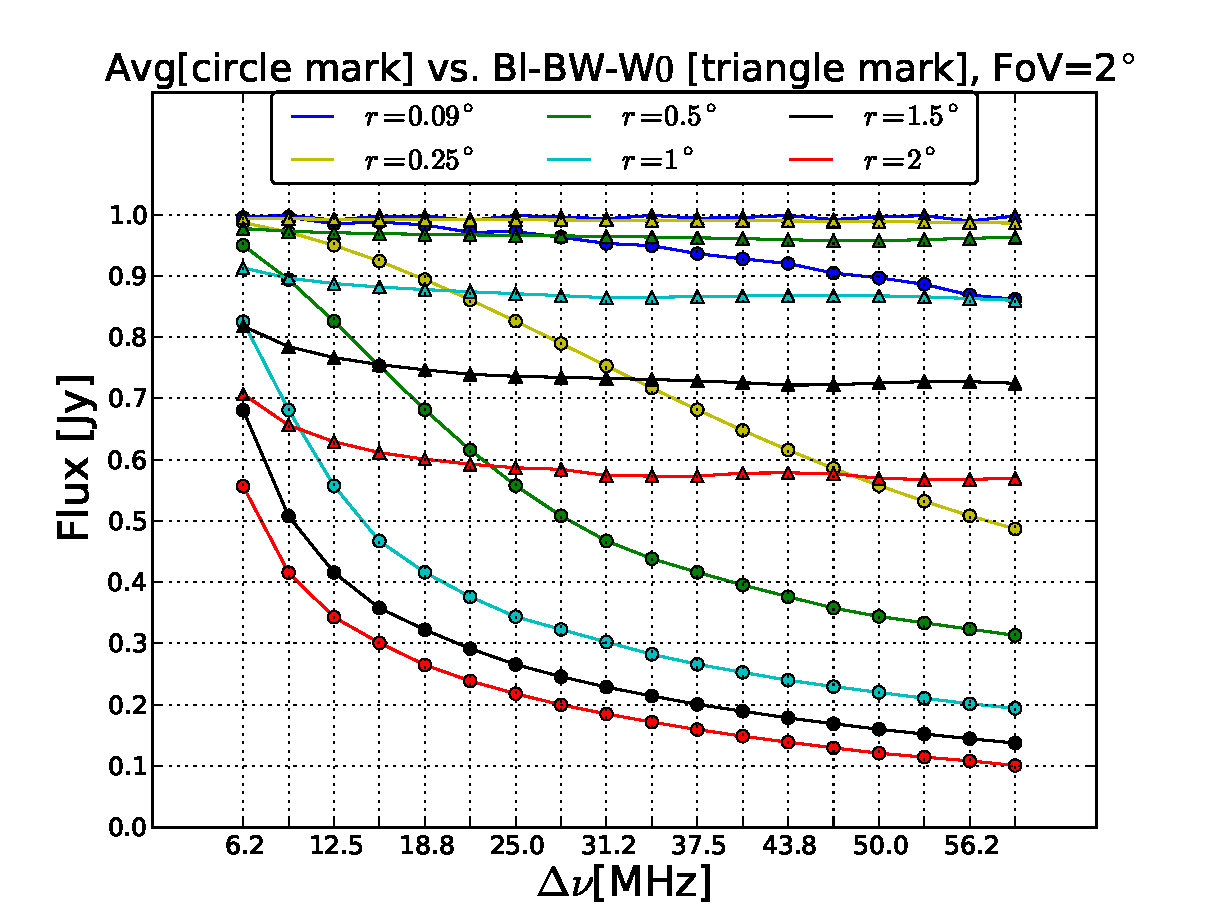
\includegraphics[width=1\textwidth]{./Figures/max-integ-freq-butter-w1x1-fov2.pdf}
      \caption{Response to a 1Jy source at different positions, as a function of bandwidth with $2^{\circ}$ frequency Butterwordth filter.}
      \label{fig:max-integ-freq-butter-w1x1-fov2}
      \end{minipage}
\hspace{1cm}
\begin{minipage}{0.36\linewidth}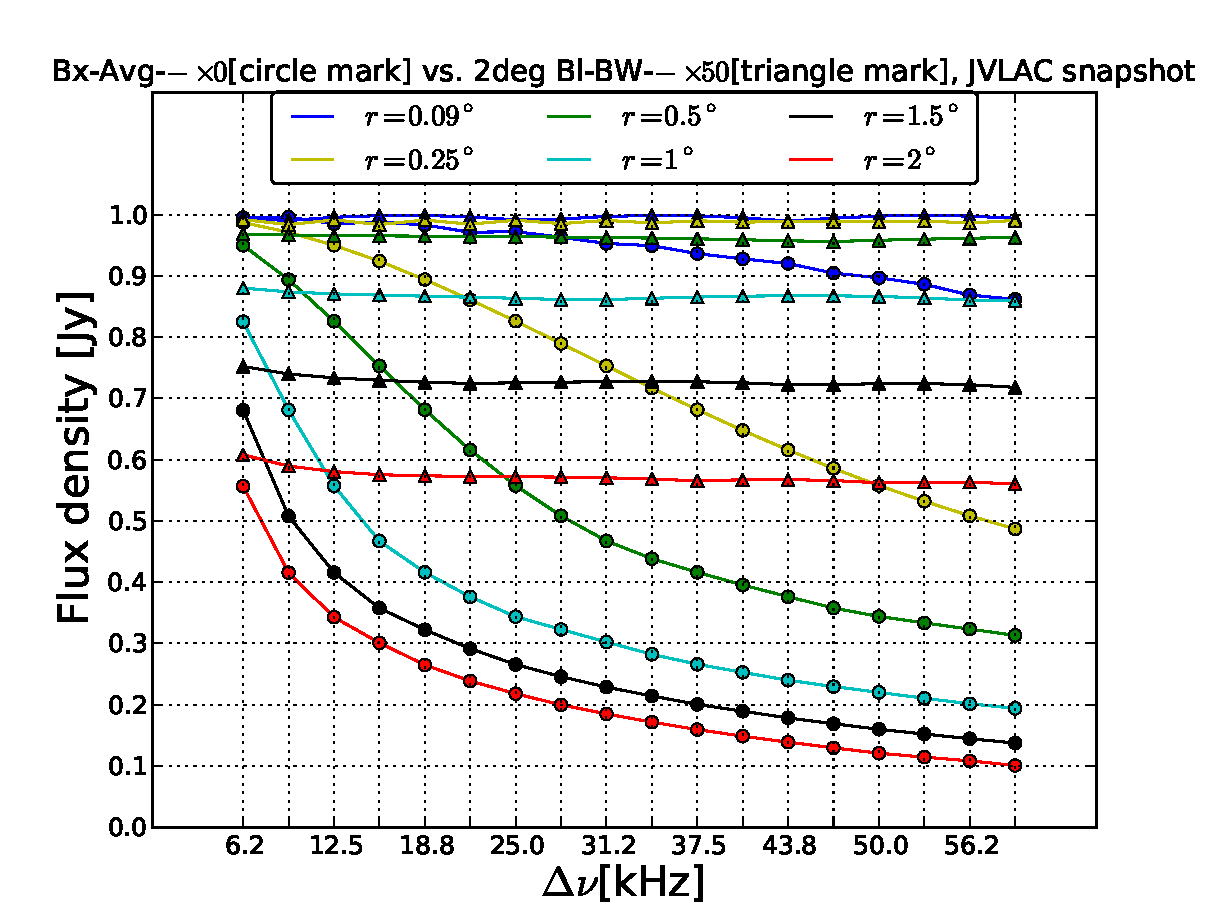
\includegraphics[width=1\textwidth]{./Figures/max-integ-freq-butter-w1x50-fov2.pdf}
      \caption{Response to a 1Jy source at different positions, as a function of bandwidth with $2^{\circ}$ frequency overlap Butterwordth 
filter.}
      \label{fig:max-integ-freq-butter-w1x50-fov2}
      \end{minipage}
\end{figure*}
\begin{figure*}
% *********************** Scripts that created these plots ***********************************
%plot.plot(wind1='/home/atemkeng/TempleFull/DATA/Maxtime-bessel-fov2-window/',title1=r'Avg[circle mark] vs. Bl-J$_0$-W$1\times 1$ [triangle 
	    %mark], FoV=2$^\circ$',xlabel=r'$\Delta t$[s]')
  \centering
\begin{minipage}{0.36\linewidth}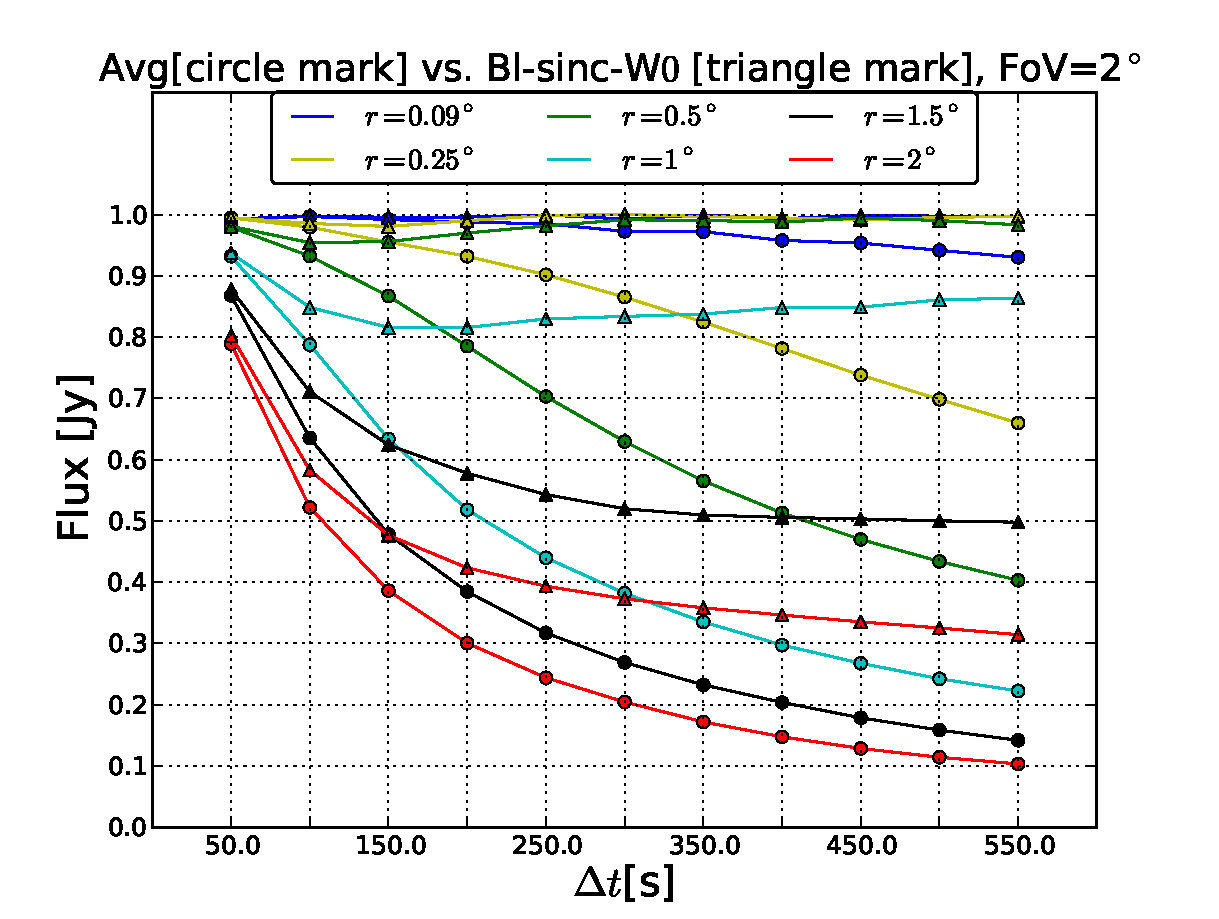
\includegraphics[width=1.\textwidth]{./Figures/max-integ-time-sinc-w1x1-fov2.pdf}
	\caption{Response to a 1Jy source at different positions, as a function of integration time with $2^{\circ}$ time sinc filter.}
	\label{fig:max-integ-time-sinc-w1x1-fov2}
	\end{minipage} \hspace{1cm}
\begin{minipage}{0.36\linewidth}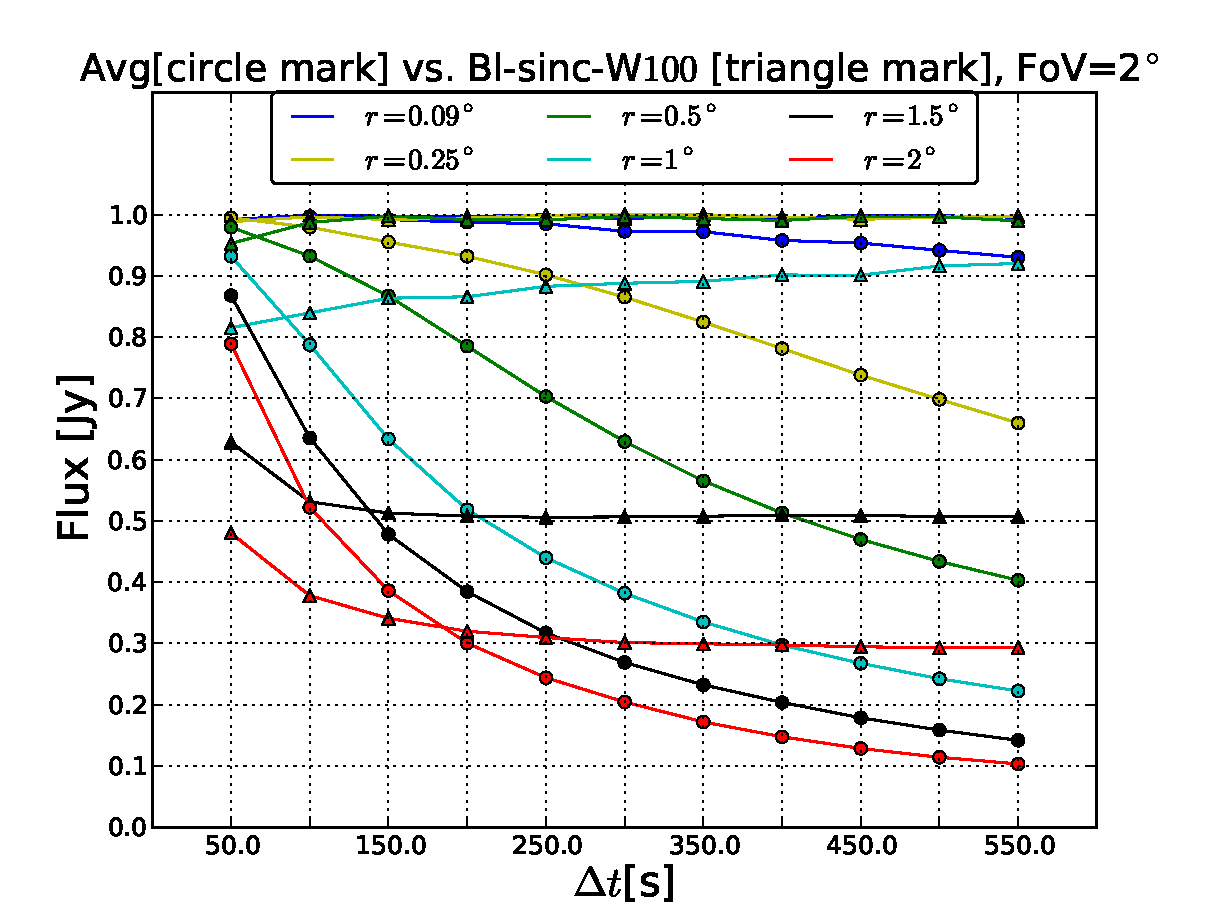
\includegraphics[width=1.\textwidth]{./Figures/max-integ-time-sinc-w100x1-fov2.pdf}
        \caption{Response to a 1Jy source at different positions, as a function of integration time with $2^{\circ}$ time overlap sinc 
filter.}
      \label{fig:max-integ-time-sinc-w100x1-fov2}
      \end{minipage}\\
\begin{minipage}{0.36\linewidth}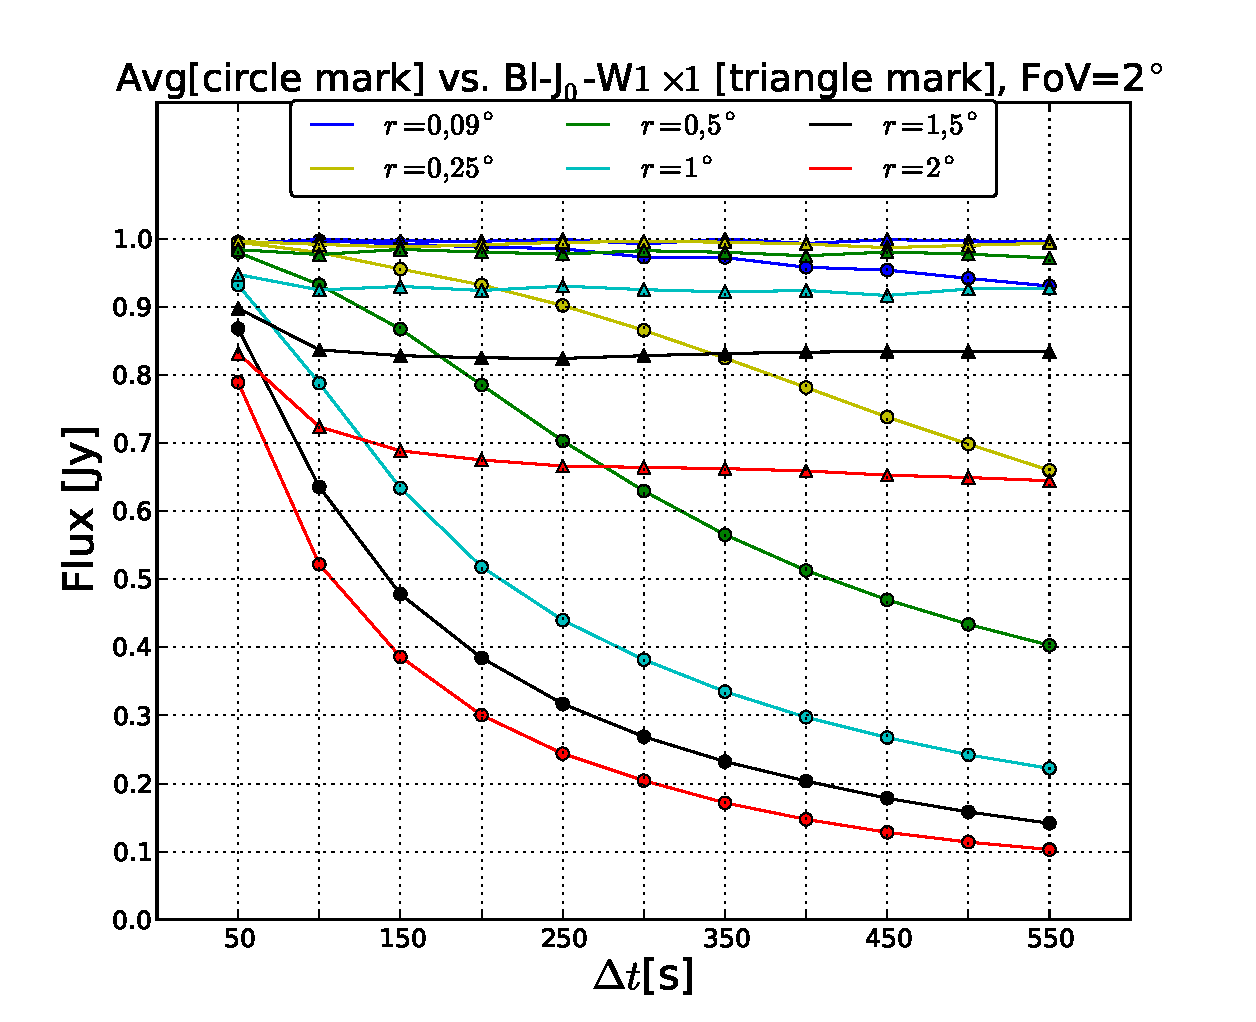
\includegraphics[width=1\textwidth]{./Figures/max-integ-time-bessel-w1x1-fov2.pdf}
    \caption{Response to a 1Jy source at different positions, as a function of integration time with $2^{\circ}$ time Bessel first kind of 
order zero
filter.}
    \label{fig:max-integ-time-bessel-w1x1-fov2}
    \end{minipage} 
 \hspace{1cm}
\begin{minipage}{0.36\linewidth}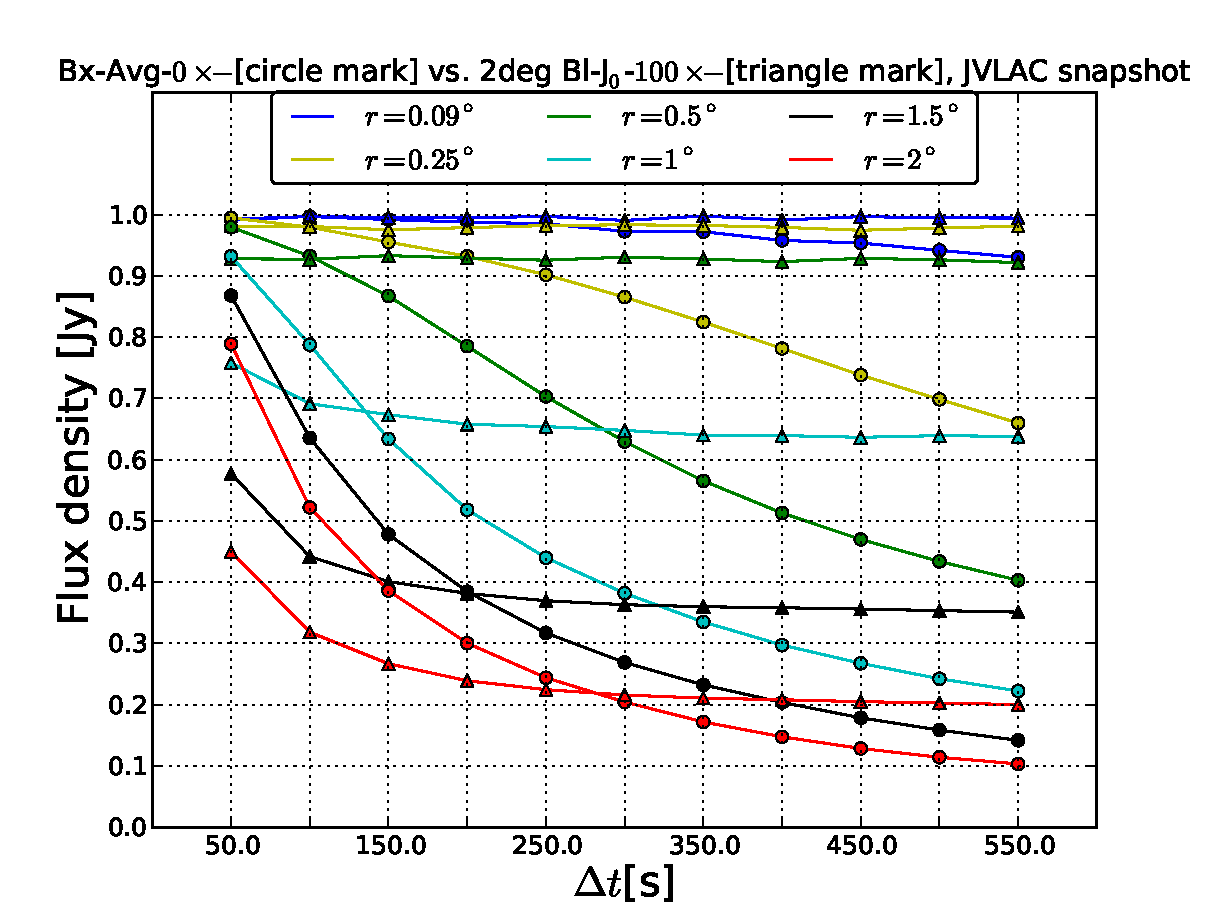
\includegraphics[width=1\textwidth]{./Figures/max-integ-time-bessel-w100x1-fov2.pdf}
    \caption{Response to a 1Jy source at different positions, as a function of integration time with $2^{\circ}$ time overlap 
      Bessel first kind of order zero filter.}
    \label{fig:max-integ-time-bessel-w100x1-fov2}\end{minipage}\\
\begin{minipage}{0.36\linewidth}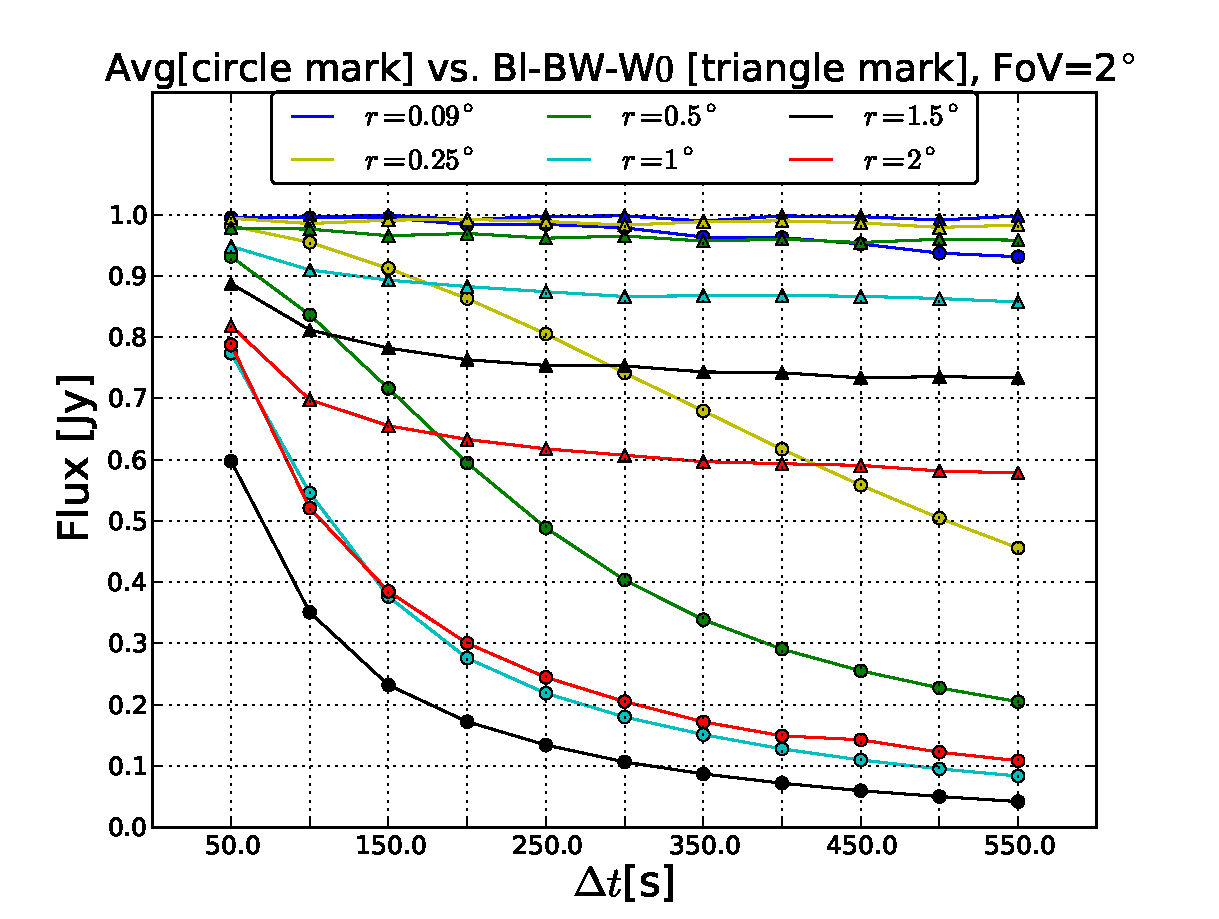
\includegraphics[width=1\textwidth]{./Figures/max-integ-time-butter-w1x1-fov2.pdf}
    \caption{Response to a 1Jy source at different positions, as a function of integration time with $2^{\circ}$ time Butterwordth 
filter.}
    \label{fig:max-integ-time-butter-w1x1-fov2}
    \end{minipage} 
 \hspace{1cm}
\begin{minipage}{0.36\linewidth}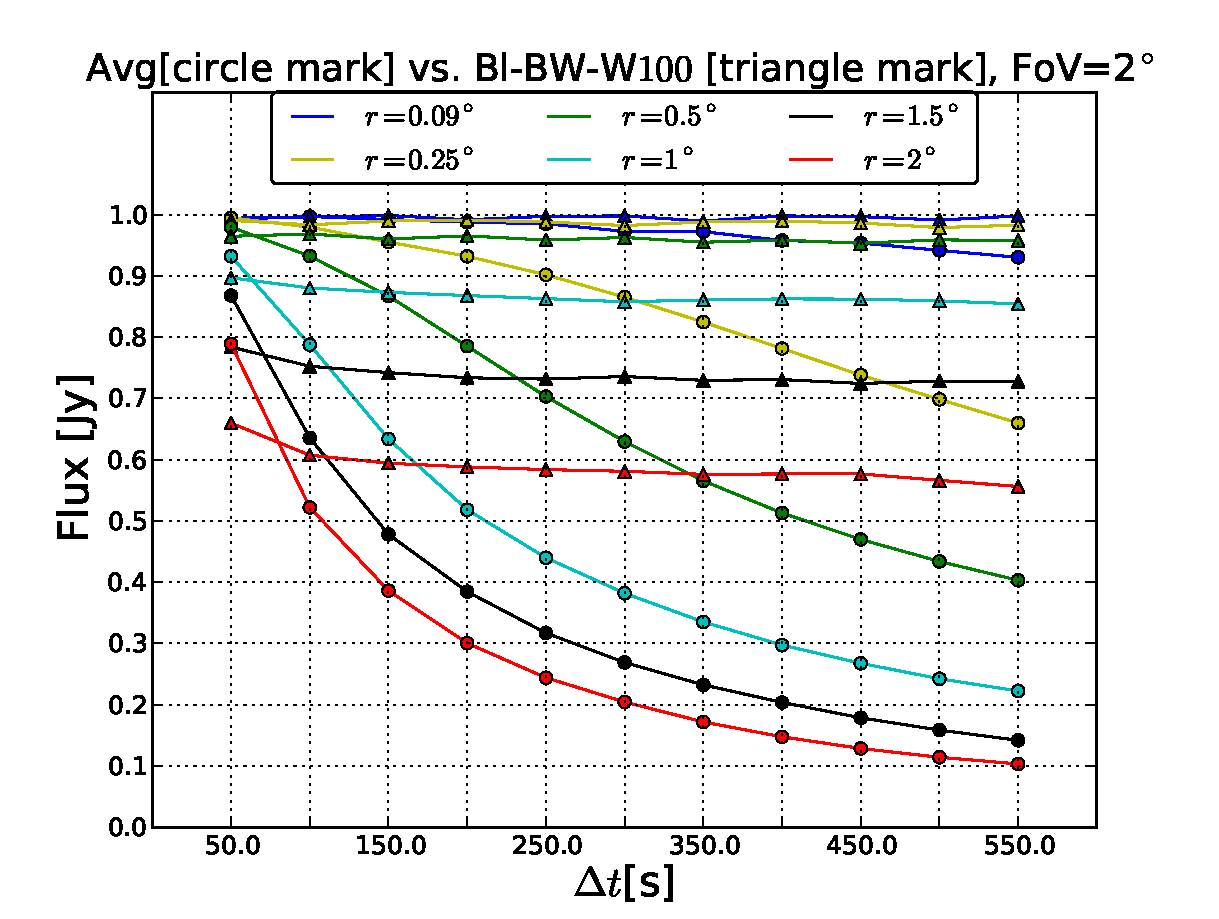
\includegraphics[width=1\textwidth]{./Figures/max-integ-time-butter-w100x1-fov2.pdf}
    \caption{Response to a 1Jy source at different positions, as a function of integration time with $2^{\circ}$ time overlap 
      Butterwordth filter.}
    \label{fig:max-integ-time-butter-w100x1-fov2}\end{minipage}   
\end{figure*}
\begin{figure*}
  \centering
\begin{minipage}{0.36\linewidth}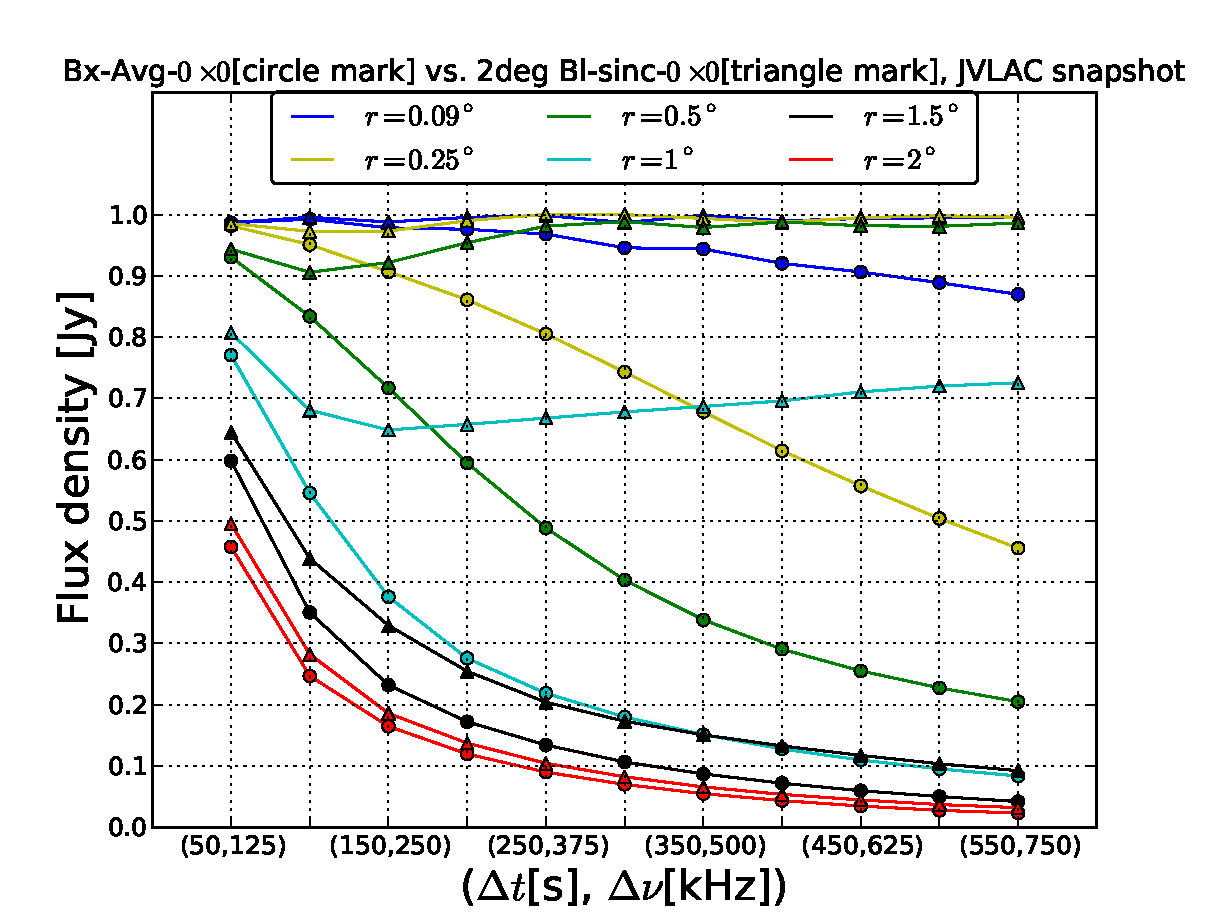
\includegraphics[width=1\textwidth]{./Figures/max-integ-timefreq-sinc-w1x1-fov2.pdf}
    \caption{Response to a 1Jy source at different positions, as a function of integration time and bandwidth; with $2^{\circ}$ frequency 
sinc filter.}
    \label{fig:max-integ-timefreq-sinc-w1x1-fov2}\end{minipage}
 \hspace{1cm}
\begin{minipage}{0.36\linewidth}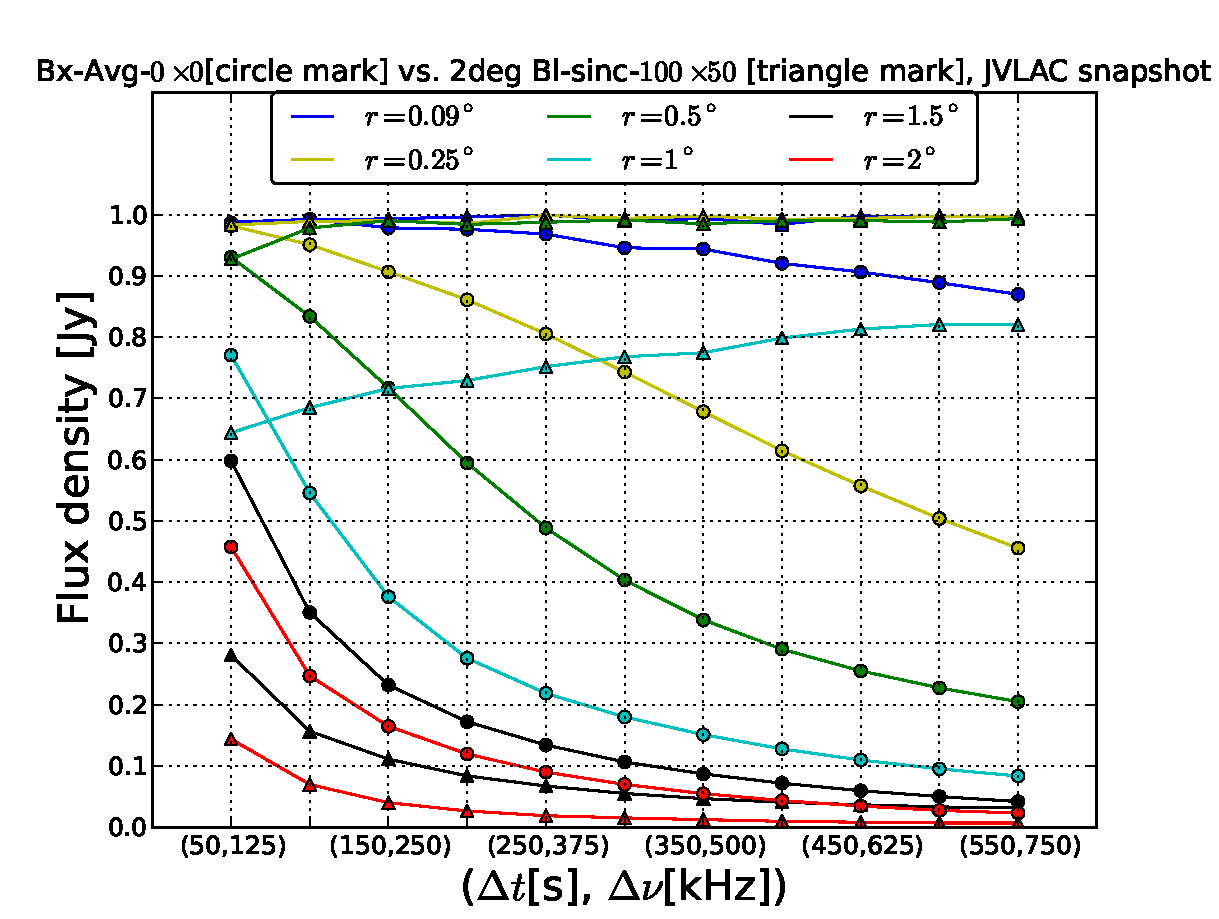
\includegraphics[width=1\textwidth]{./Figures/max-integ-timefreq-sinc-w100x50-fov2.pdf}
    \caption{Response to a 1Jy source at different positions, as a function of integration time and bandwidth; with $2^{\circ}$ frequency 
 overlap sinc filter.}
    \label{fig:max-integ-timefreq-sinc-w100x50-fov2}\end{minipage}\\
\begin{minipage}{0.36\linewidth}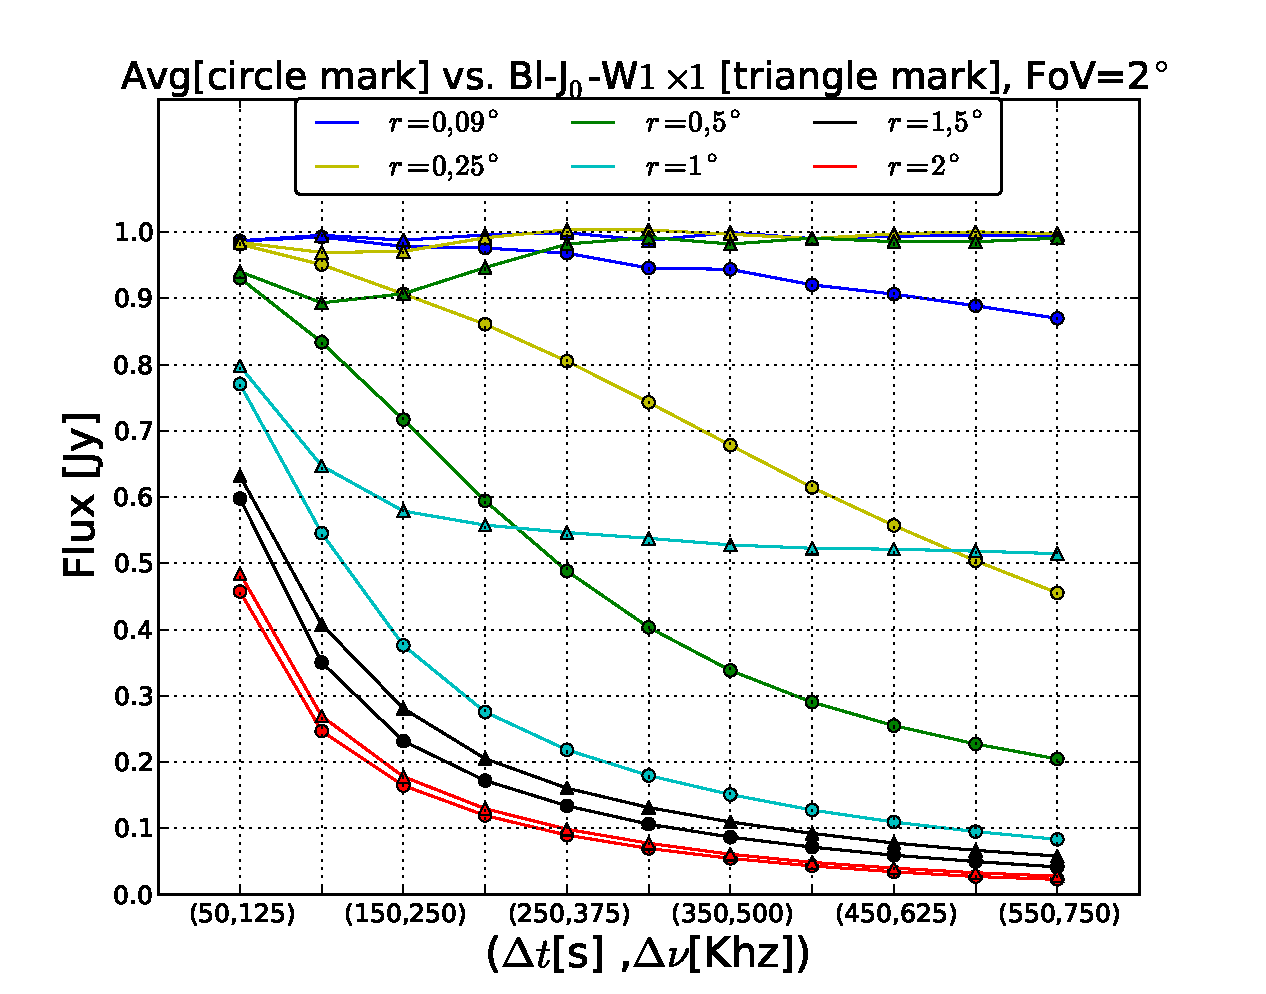
\includegraphics[width=1\textwidth]{./Figures/max-integ-timefreq-bessel-w1x1-fov2.pdf}
      \caption{Response to a 1Jy source at different positions, as a function of integration time and bandwidth, with $2^{\circ}$ frequency 
Bessel first kind of order zero filter.}
      \label{fig:max-integ-timefreq-bessel-w1x1-fov2}\end{minipage}
\hspace{1cm}
\begin{minipage}{0.36\linewidth}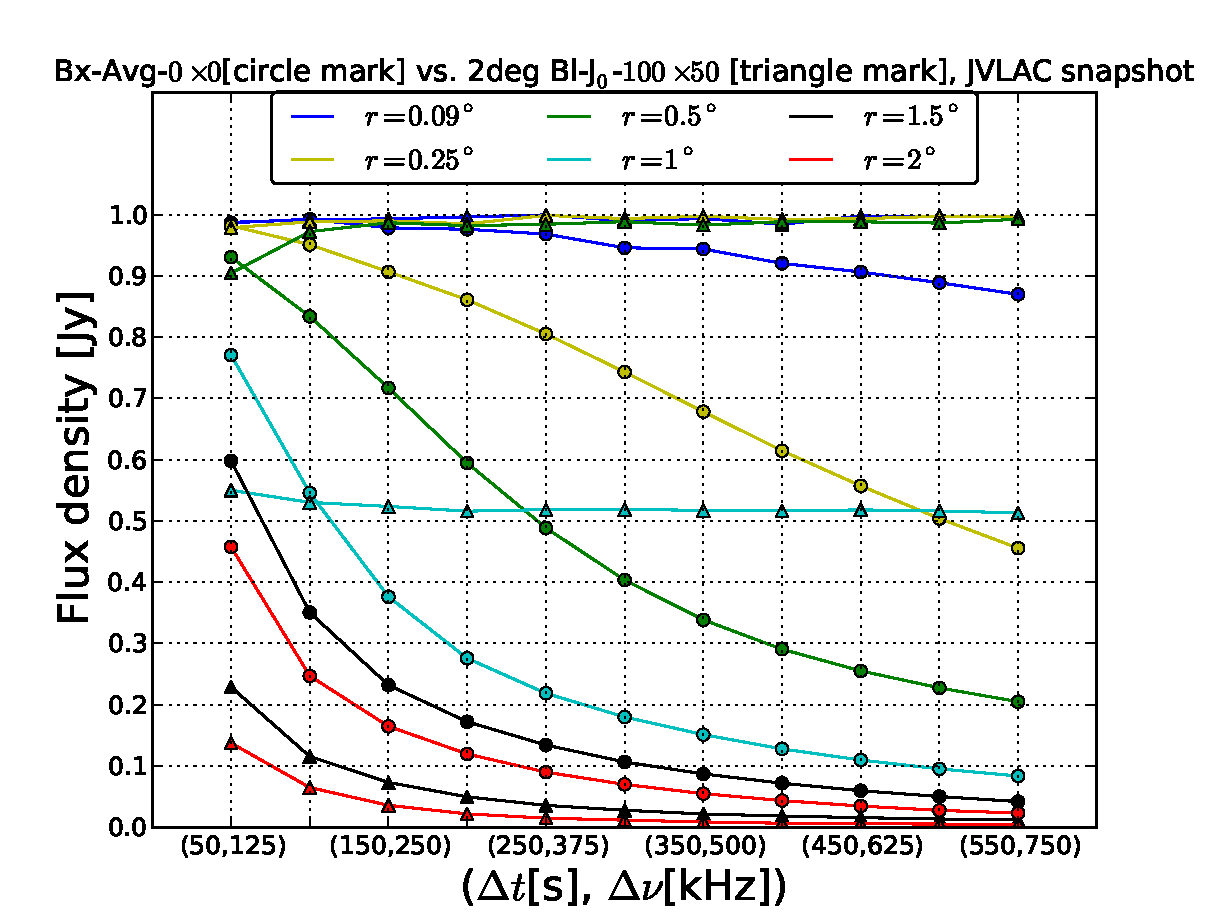
\includegraphics[width=1\textwidth]{./Figures/max-integ-timefreq-bessel-w100x50-fov2.pdf}
      \caption{Response to a 1Jy source at different positions, as a function of integration time and bandwidth, with $2^{\circ}$ frequency 
overlap Bessel first kind of order zero filter.}
  \label{fig:max-integ-timefreq-bessel-w100x50-fov2}\end{minipage}
\begin{minipage}{0.36\linewidth}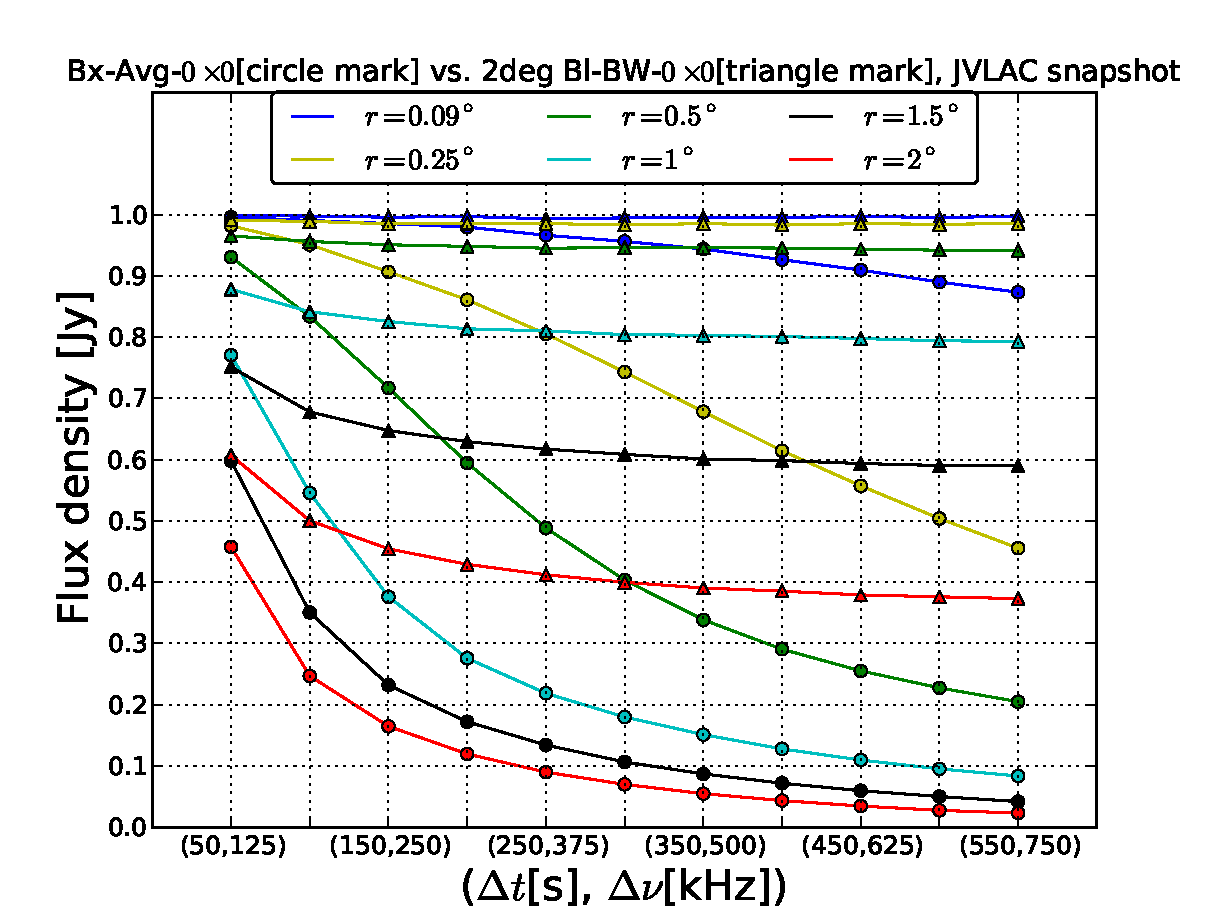
\includegraphics[width=1\textwidth]{./Figures/max-integ-timefreq-butter-w1x1-fov2.pdf}
      \caption{Response to a 1Jy source at different positions, as a function of integration time and bandwidth, with $2^{\circ}$ frequency 
Butterwordth filter.}
      \label{fig:max-integ-timefreq-butter-w1x1-fov2}\end{minipage}
\hspace{1cm}
\begin{minipage}{0.36\linewidth}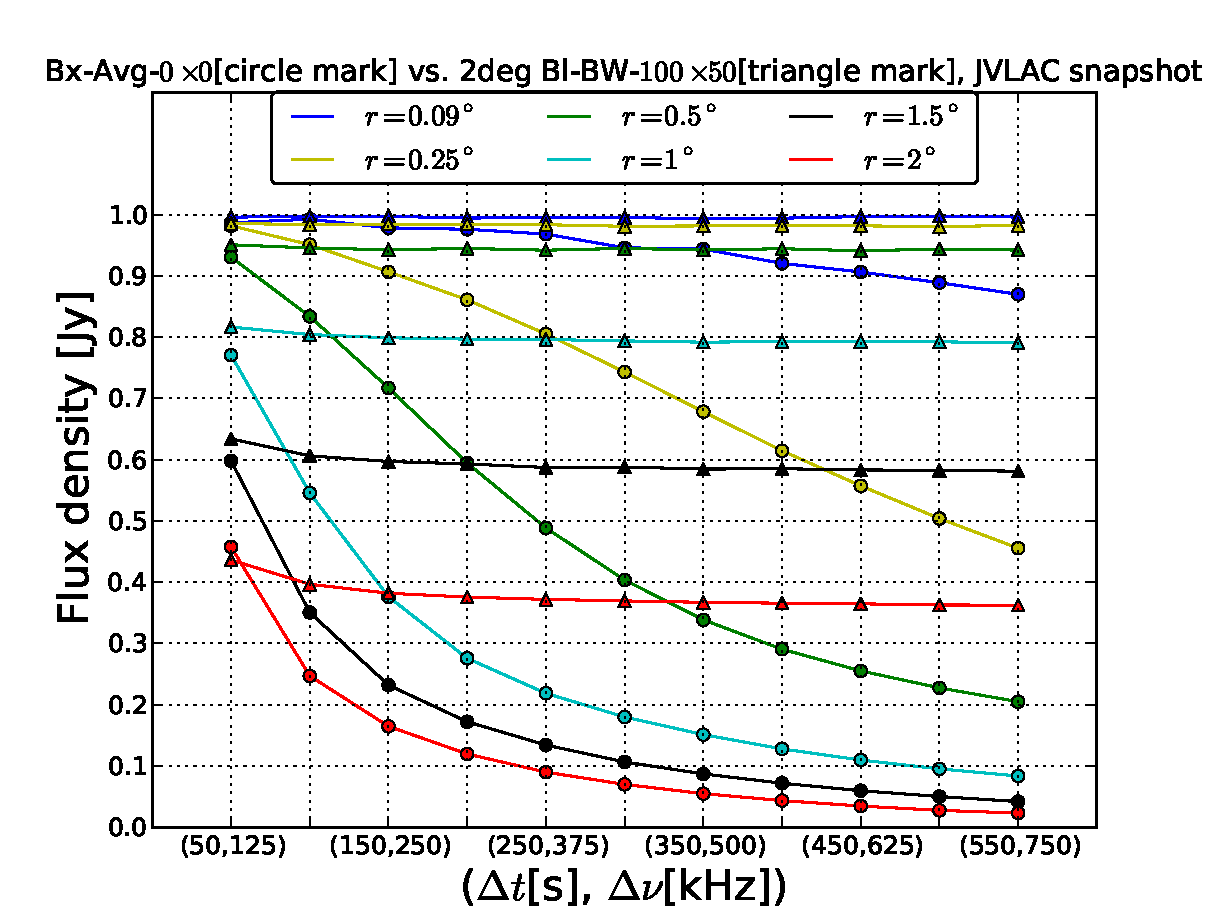
\includegraphics[width=1\textwidth]{./Figures/max-integ-timefreq-butter-w100x50-fov2.pdf}
      \caption{Response to a 1Jy source at different positions, as a function of integration time and bandwidth, with $2^{\circ}$ frequency 
overlap Butterwordth filter.}
  \label{fig:max-integ-timefreq-butter-w100x50-fov2}\end{minipage}
\end{figure*}
\section{Conclusions}
The goal of this paper was threefold. The first goal was to investigate **** windowing functions***\\
The second objective  was to study ****first algorithm data compression***\\
The final objective was to ****second algorithm data compression and out field suppression*** \\
Drawback and futures works*** drawback and futures works*****
\section*{Acknowledgements}
\bibliographystyle{mn2e}
\bibliography{m_paper}
\appendix
\section[]{Derivation of complex matrices}
\label{app:complexmatrices}
The complex matrices used in section \ref{sec:imaging} are explicitly derived in this appendix. In Eq.\ref{eqbb:linear}, the matrices
$\mathbf{C}_{(t,\nu)}^{block}$ and $\mathbf{W}_{pq,(t,\nu)}^{block}$ are blocks diagonals  both of size $(4n_t n_{\nu})\times(4n_t 
n_{\nu})$, and  the sampled visibilities $\mathbf{V}_{pq,(t,\nu)}^{samp}$ is a vector of size $4\times (n_t n_{\nu})$. These matrices are 
explicitly expressed as follow:
\begin{equation*}
\mathbf{C}_{(t,\nu)}^{block}=
  \begin{bmatrix}
    \mathbf{c}_{(t,\nu)} & 0 & 0 & 0\\
    0 &  \mathbf{c}_{(t,\nu)} &0 & 0 \\
    0 & 0 & \mathbf{c}_{(t,\nu)} & 0\\
      0 & 0 & 0 & \mathbf{c}_{(t,\nu)}\\
  \end{bmatrix}
\end{equation*}
\begin{equation*}
\mathbf{W}_{pq,(t,\nu)}^{block}=
  \begin{bmatrix}
    \mathbf{W}_{pq,(t,\nu)}& 0 & 0 & 0\\
    0 &  \mathbf{W}_{pq,(t,\nu)} &0 & 0 \\
    0 & 0 & \mathbf{W}_{pq,(t,\nu)} & 0\\
      0 & 0 & 0 & \mathbf{W}_{pq,(t,\nu)}\\
  \end{bmatrix}
\end{equation*}
\begin{eqnarray*}
\mathbf{V}_{pq,(t,\nu)}^{samp}&=&\Bigg[\mathcal{V}_{pq,(t,\nu)}^{0},\mathcal{ V } 
^1_{pq,(t,\nu)},\mathcal{V}^2_{pq,(t,\nu)},\mathcal{V}_{pq,(t,\nu)}^{3 } \Bigg]^T. 
\end{eqnarray*}
In Eq.\ref{eq2:block}, the matrices $\mathbf{C}_{(t,\nu)}^{block,n}$ and 
$\mathbf{W}_{pq,(t,\nu)}^{block,n}$ are blocks diagonals both of size $(4N_v^{pq}n_t n_{\nu})\times (4N_v^{pq}n_t n_{\nu})$, and 
the sampled visibilities $\mathbf{V}_{pq,(t,\nu)}^{samp,n}$ is a one row matrix of size $(N_v^{pq}4 n_t n_{\nu})\times (4 n_t n_{\nu})$ 
made of $\textbf{V}_{pq,(t,\nu)}^{samp}$. These matrices are explicitly expressed as follow:
\begin{equation*}
\mathbf{C}_{(t,\nu)}^{block,n}=
  \begin{bmatrix}
    \mathbf{C}_{(t,\nu)}^{block} &\dots & 0 & \dots & 0\\
    \vdots & \vdots & \vdots & \vdots & \vdots\\
    0 & \dots& \mathbf{C}_{(t,\nu)}^{block} &\dots & 0\\
    \vdots & \vdots & \vdots & \vdots & \vdots \\
    0 & \dots& 0 &\dots & \mathbf{C}_{(t,\nu)}^{block}\\
  \end{bmatrix}
\end{equation*}
\begin{equation*}
\mathbf{W}_{pq,(t,\nu)}^{block,n}=
  \begin{bmatrix}
    \mathbf{W}_{pq,(t,\nu)}^{block} &\dots & 0 & \dots & 0\\
    \vdots & \vdots & \vdots & \vdots & \vdots\\
    0 & \dots& \mathbf{W}_{pq,(t,\nu)}^{block} &\dots & 0\\
    \vdots & \vdots & \vdots & \vdots & \vdots \\
    0 & \dots& 0 &\dots & \mathbf{W}_{pq,(t,\nu)}^{block}\\
  \end{bmatrix}
\end{equation*}
\begin{eqnarray*}
\mathbf{V}_{pq,(t,\nu)}^{samp,n}&=&\Bigg[\mathbf{V}_{pq,(t,\nu)}^{samp},\dots, \mathbf{V}_{pq,(t,\nu)}^{samp}, \dots,
\mathbf{V}_{pq,(t,\nu)}^{samp}\Bigg]^T. 
\end{eqnarray*}
In Eq.\ref{eq:noise}, the matrix $\mathbf{B}$ of size $(N_v 4 n_t n_{\nu})\times (4 n_t n_{\nu})$ is defined as follow
\begin{equation*}
\mathbf{B}_{}=
  \begin{bmatrix}
    \mathbf{C}_{(t,\nu)}^{block,n}\cdot \mathbf{W}_{01,(t,\nu)}^{block,n}\cdot \mathbf{S}_{01,(t,\nu)}^{n}\\
    \vdots\\
    \mathbf{C}_{(t,\nu)}^{block,n}\cdot \mathbf{W}_{ik,(t,\nu)}^{block,n}\cdot \mathbf{S}_{ik,(t,\nu)}^{n}\\
    \vdots \\
    \mathbf{C}_{(t,\nu)}^{block,n}\cdot \mathbf{W}_{jl,(t,\nu)}^{block,n}\cdot \mathbf{S}_{jl,(t,\nu)}^{n}
  \end{bmatrix}
\end{equation*}
\section[]{Sky tapering function with averaging}
\label{label:similarimaging}
The measured sky intensity of the array is derived from the inverse Fourier transform of the sum of the sample visibilities 
measured at each baseline.
\begin{eqnarray*}
 \mathcal{I}^{D}_{l,m}&=& \mathcal{F}^{-1}\Bigg\{\sum_{pq} c_{pq,(t,\nu)}\cdot\Big(\Pi_{pq}\circ V_{pq}^{samp}\Big)_{(t,\nu)}\Bigg\}\\
		      &=&\sum_{pq} \mathcal{F}^{-1}\{c_{pq,(t,\nu)}\}\circ \Big(\mathcal{F}^{-1}\{\Pi_{pq,(t,\nu)}\}\cdot 
\mathcal{F}^{-1}\{V_{pq,(t,\nu)}^{samp}\}\Big)
\end{eqnarray*}
\begin{eqnarray*}	     
\mathcal{I}^{D}_{l,m}&=&\sum_{pq}\mathcal{F}^{-1}\{\Pi_{pq,(t,\nu)}\}\cdot\bigg(\mathcal{F}^{-1}\{S_{pq}\cdot V_{pq,(t,\nu)}\}
\bigg)
\end{eqnarray*}
recall from section \ref{sec:AvgCon} that $S_{pq}$ is the sampling function of the baseline $pq$ and $\Pi_{pq,(t,\nu)}$ is the 
boxcar window.  This can be re-written as
\begin{eqnarray*}	     
\mathcal{I}^{D}_{l,m}&=&\sum_{pq} \mathcal{R}_{pq} \cdot\bigg(\mathcal{B}_{pq}\circ \mathcal{I}^{sky}_{l,m}\bigg)
\end{eqnarray*}
If all baselines are seen the same sky, then we can write:
\begin{eqnarray*}	     
\mathcal{I}^{D}_{l,m}&=&\mathcal{R}_{}\cdot\Bigg(\bigg(\sum_{pq}\mathcal{B}_{pq}\bigg)\circ \mathcal{I}^{sky}_{l,m}\Bigg)
\end{eqnarray*}
Here, $\mathcal{B}_{pq}$ is the point spread function for the baseline $pq$ and $\mathcal{R}_{pq}= \mathcal{R}$ is the sky taper, where 
$\mathcal{R}_{}=sinc$.\\
\\
\bsp
\label{lastpage}
\end{document}
